\documentclass[12pt, titlepage]{article}

\usepackage[margin = 1in]{geometry}
\usepackage{amsmath}
\allowdisplaybreaks
\usepackage{authblk}
\usepackage{setspace}
\usepackage{natbib}
\usepackage{hyperref}\hypersetup{colorlinks=true, citecolor=blue}
\usepackage{parskip}
\usepackage{textgreek}
\usepackage{graphicx}
\usepackage{booktabs} % For better looking tables
\usepackage{siunitx} % For alignment of numbers
\usepackage{placeins}
\usepackage{caption}  % For custom captions
\usepackage{float}   % Required for the H specifier
\usepackage{adjustbox}
\usepackage[]{lineno}
\linenumbers*[1]

%% patches to make lineno work better with amsmath
\newcommand*\patchAmsMathEnvironmentForLineno[1]{%
	\expandafter\let\csname old#1\expandafter\endcsname\csname
	#1\endcsname
	\expandafter\let\csname oldend#1\expandafter\endcsname\csname
	end#1\endcsname
	\renewenvironment{#1}%
	{\linenomath\csname old#1\endcsname}%
	{\csname oldend#1\endcsname\endlinenomath}}%
\newcommand*\patchBothAmsMathEnvironmentsForLineno[1]{%
	\patchAmsMathEnvironmentForLineno{#1}%
	\patchAmsMathEnvironmentForLineno{#1*}}%
\AtBeginDocument{%
	\patchBothAmsMathEnvironmentsForLineno{equation}%
	\patchBothAmsMathEnvironmentsForLineno{align}%
	\patchBothAmsMathEnvironmentsForLineno{flalign}%
	\patchBothAmsMathEnvironmentsForLineno{alignat}%
	\patchBothAmsMathEnvironmentsForLineno{gather}%
	\patchBothAmsMathEnvironmentsForLineno{multline}%
}

\sisetup{
    group-separator = {,},
    round-mode = places,
    round-precision = 2,
    output-decimal-marker = {.},
    table-number-alignment = center,
    table-figures-integer = 6,
    table-figures-decimal = 2,
    table-figures-uncertainty = 2
}

% image path
\graphicspath{{.}{./images}}

% control floats
\renewcommand\floatpagefraction{.9}
\renewcommand\topfraction{.9}
\renewcommand\bottomfraction{.9}
\renewcommand\textfraction{.2}
\setcounter{totalnumber}{50}
\setcounter{topnumber}{50}
\setcounter{bottomnumber}{50}

\newcommand{\jy}[1]{\textcolor{orange}{JY: (#1)}}
\newcommand{\yh}[1]{\textcolor{purple}{YH: (#1)}}
\newcommand{\yx}[1]{\textcolor{cyan}{YX: (#1)}}
\let\proglang=\textsf
%% \newcommand{\pkg}[1]{{\fontseries{m}\selectfont #1}}
%% \newcommand\code[2][black]{\textcolor{#1}{\texttt{#2}}}

\title{Principles for Open Data Curation: A Case Study with the New
  York City 311 Service Request Data}


\author[1]{David Tussey}
\author[2]{Jun Yan}
\affil[1]{Former Executive Director, NYC DoITT}
\affil[2]{Department of Statistics, University of Connecticut}


\begin{document}
\maketitle

\tableofcontents % Optional: Table of Contents
\listoffigures % List of Figures
\listoftables % List of Tables

\hyphenpenalty=1000

\begin{abstract}
  In the early 21st century, the open data movement began to transform societies and governments through principles of transparency, 
  innovation, and public engagement. New York City (NYC) has emerged as a leader in this movement 
  with the enactment of the Open Data Law in 2012, leading to the creation of the NYC Open Data portal, 
  which now hosts 2700 datasets from 80 city agencies. This resource has proven invaluable for research 
  across various domains, including health, urban development, and transportation. 
  The success of these initiatives underscores the importance of data curation, ensuring the utility and reliability of datasets. 

This paper examines the data curation challenges using the NYC 311 Service Request (SR) Data as a case study, 
  addressing issues of data validity, consistency, and curation efficiency. Based on insights from this case study, 
  we propose a set of data curation principles tailored for government-released open data. 
  These principles aim to enhance data management practices and ensure the ongoing utility of open data. 
  The paper concludes with actionable suggestions for improving data curation 
  and offers general principles for the release of open data.

\bigskip
  
\noindent
\textit{Keywords:}
311 Service Request Data;
Data cleansing;
Data Consistency;
Data Curation;
Data Democratization;
Data Efficiency;
Data science;
Data Validity;
Government Data;
NYC Open Data;
Open Data Movement;
Open data;
Public Engagement;
Quality control;
Research Data Management;
Smart Cities;
Transparency;
\end{abstract}

\doublespacing

\section{Introduction} \label{sec:intro}

In the early 21st century, the open data movement began to take shape, driven by the 
fundamental belief that freely accessible data can transform 
both societies and governments. This movement champions the principles of 
transparency, innovation, and public engagement. 
A landmark in this journey was the launch of the United States'
\href{https://www.data.gov}{Data.gov} portal in 2009, a pioneering
platform in making government data widely accessible. Shortly after,
the European Union followed suit, unveiling its
\href{https://data.europa.eu/euodp}{Open Data Portal} in 2012, further
cementing the movement's global reach. Furthermore, the World Bank's Open
Data initiative, initiated in 2010, stands out as a comprehensive
repository for global development data, available at
\href{https://data.worldbank.org}{World Bank Open Data}. 
These initiatives represent significant strides in democratizing data, in breaking barriers that once
kept valuable information on government performance in silos. Their collective impact is profound, extending beyond
mere data sharing to fostering a culture of openness that benefits
individuals, communities, governments, and economies worldwide
\citep{barns2016mine, wang2016adoption}.


New York City (NYC) has emerged as a forerunner in the open data
movement, marked by the enactment of the Open Data Law in 2012
\citep{zuiderwijk2014open}. This landmark legislation led to the
creation of the \href{https://opendata.cityofnewyork.us}{NYC Open Data
  portal}, which today hosts an impressive array of 2700 datasets
from 80 different city agencies. This resource has become invaluable
for researchers in various fields as well an enabling local government transparency

In health, datasets have enabled
significant studies on facets of health and healthcare delivery
\citep{cantor2018facets, shankar2021data}. In the realm of urban
development, data has been instrumental in advancing smart city
initiatives \citep{neves2020impacts}. Additionally, transportation
research has benefited greatly from this wealth of data, aiding in the
understanding of urban mobility and infrastructure
\citep{gerte2019understanding}. NYC's Open Data initiative not only
exemplifies commitment to transparency and public engagement but also
illustrates how open data can be a powerful tool in addressing complex
urban challenges. Examples of some of the more popular NYC datasets include:

\begin{itemize}
	\item NYC restaurant violations
	\item Popular baby names
	\item Mapping of car crashes involving pedestrians
	\item Mapping of sidewalk widths in NYC 
	\item Visualization of NYC High School and College enrollment
	\item An interactive dashboard to filter and view charges for jail inmates
	\item Location of City-wide free Internet access points
	\item ...and 220 other complaint types. 
\end{itemize}

Data curation is fundamental in the open data ecosystem, ensuring the
utility and reliability of datasets for diverse applications. Among
the earliest discussions, \citet{witt2009constructing} focus on the
development of data curation profiles tailored to specific contexts,
setting a precedent for targeted data management
strategies. Addressing broader challenges in data sharing and
management, \citet{borgman2012conundrum} highlights the complexities
of research data distribution, emphasizing the need for robust
strategies. This is complemented by the work of \citet{hart2016ten},
who outline essential principles for effective data management,
particularly emphasizing the importance of meticulous curation
practices. 

In the realm of collaborative data management,
\citet{beheshti2019datasynapse} underscore the significance of
cooperative environments for managing and sharing social data
effectively. This aspect of data curation gains further relevance in
the research by \citet{mclure2014data}, which delves into the specific
practices and needs within data curation communities. The practical
implications of data curation are vividly illustrated in the context
of public health and global challenges. \citet{cantor2018facets}
demonstrate the utility of curated open data in evaluating community
health determinants. Furthermore, the COVID-19 pandemic serves as a
real-world example, with \citet{shankar2021data} observing the
critical role of collective data curation efforts in managing and
responding to the crisis. Collectively, these studies not only highlight the 
multifaceted nature of data curation but also emphasize
its indispensable role in enhancing the applicability and value of
open data across various domains.


The contributions of this paper are twofold. First, we delve into
the specifics of data curation challenges using the NYC 311 Service
Request (SR) Data as a case study. This renowned and frequently viewed 
dataset serves as a prime example for examining key issues in data curation, 
including data validity, consistency, and curation efficiency. 
We illustrate these points with live examples drawn from our processing of the 311 SR data. 
Secondly, building upon insights gained from this case study, we 
propose a set of data curation principles tailored for government-released open data. 
These principles are designed to address the unique challenges 
and requirements observed in the curation of such datasets.


The paper is organized as follows:
Section~\ref{sec:history} offers a brief review of the history of the 311 system. In 
Section~\ref{sec:trends} we take a look at long-term trends presented via a 10-year analysis.
Section~\ref{sec:issues} offers a general discussion of data cleansing issues
impacting data quality and curation efficiency. Section~\ref{sec:structural} examines
the technical dimensions of the dataset, the structural issues. In Section~\ref{sec:datatypes} we examine the data fields
for compliance with the stated data type as found in the Data Dictionary. Section~\ref{sec:blanks} looks
at the data fields as regards missing, blank, or N/A entries. Section~\ref{sec:domain} explores
how data fields comply with a domain of legal or acceptable values. Section~\ref{sec:inconsistencies}
deals with the important issues surrounding logical inconsistencies and concerning patterns in the data. Section~\ref{sec:precision} 
explores the age-old issue of precision versus accuracy. Section~\ref{sec:duplicates}
identifies duplicate and redundant data fields. Section~\ref{sec:improvements} provides 
actionable suggestions for mitigating or resolving identified issues. Following this, Section~\ref{sec:protocol} outlines a series of general 
principles for the release of open data, drawing from our findings. The paper concludes with a discussion 
in Section~\ref{sec:discussion}, encapsulating the key insights and implications of our research.

A note on naming conventions: dataset field names are typically named using ``snake\_case'' where
each word in the variable name is written in lowercase, and words are separated by underscores,
e.g created\_date, complaint\_type, zip\_code, etc..   



\section{NYC 311 System History} \label{sec:history}

The NYC 311 service, a critical component of New York City's public
engagement and service response framework, serves as a centralized hub
for non-emergency inquiries and requests. Introduced in 2003, the NYC
311 system was designed to streamline the city's response to
non-emergency issues, ranging from noise complaints to street
maintenance requests. The evolution of this system can be traced from
its initial implementation as a simple inquiry channel via telephone to a
comprehensive data management system that handles millions of requests
annually. Each inquiry is logged as a complaint in the 311 system.
Key milestones in the 311 system development include:

\begin{itemize}
 	\item 2003 - NYC 311 system goes live with a phone-based call center only. The ``311'' phone number replaces a myriad of numbers to call for each individual City Agency.
   	\item 2009 - 311 online \& mobile apps launched. Today 60\% of all Service Requests come from mobile \& online channels.
   	\item 2019 - Major software upgrade of 311 system with enhanced capabilities, dynamic load-balancing, and cloud-based resilience. Only major software upgrade since 2004.	
      \item 2020 - In August 2020, driven by the COVID pandemic, monthly 311 Service Requests hit an all-time high of 348,463. Seven of the Top 10 busiest days of all-time occur in 2020.
      \item 2021 - 311 System is expanded to into the MTA's city subway system, the largest expansion since its inception.
   	\item 2023 - Record high year for 311 with 3.23 million Service Requests.
\end{itemize}

Today, the NYC 311 data system is a robust platform that manages a
vast array of urban living-related inquiries. The system handles over 3 million service 
requests (SRs) per year, encompassing such complaints as street noise, illegal parking, heat/hot water, abandoned vehicles,
and unsanitary conditions. The data, managed through a tailored application built on the 
Microsoft Dynamics and Azure platform, is a valuable resource for city
administration and policy-making. The 311 data is publicly accessible through the 
NYC Open Data Portal which provides access
to all the data sets (approx. 2700) and provides a convenient method for querying, grouping, aggregating, geo-mapping, visualization, and exporting
results. This open data initiative enables not only governmental transparency but also empowers 
researchers, civic developers, and the general public. 

Additional Open Data projects can be found at \href{https://opendata.cityofnewyork.us/projects/}{NYC Open Data Project Gallery}
and at \href{https://beta.nyc/beta/products/}{\textbeta etaNYC} products and tools.

Despite its success, the system constantly faces challenges such as:

\begin{itemize}
	\item Data timeliness, accuracy, and consistency
	\item Difficulties correlating data over long time periods, e.g. over a 10-year period, e.g. Agency name changes, new complaint types.
	\item Data anonymization and handling of Personally identifiable information (PII)
	\item Integration with stand-alone systems at selected NYC Agencies
	\item Managing API usage, authentication, and load for 3\textsuperscript{rd} party users, of which there are many
	\item Incorporating ongoing technology changes and upgrades 
	\item Understanding the role of chatbots and AI to provide online customer service, along with other emergent technologies
\end{itemize}

These and other challenges are continually addressed by the various Agency open data managers
as well as the \href{https://www.nyc.gov/content/oti/pages/}{NYC Office of Technology and Innovation (OTI)} which
provides the technology support for the open data system.  
Many of the underlying datasets are updated daily, usually running 1-2 days behind from creation.
However, a number of datasets are updated monthly (such as restaurant inspections), and some are
not updated for one or more years (such as community board boundaries). This poses problems when 
merging dataset with others, as would be expected. Typically, the data must be
exported and manipulated in another, external program. The authors found this to be the case with 
the large 311 dataset employed.

Data accuracy and consistency is typically established between OTI and the other contributing
City Agencies, such as NYPD, Housing Preservation and Development (HPD), Parks \& Recreation, etc.,
via Service Level Agreements (SLAs). However, enforcement of those SLAs is often challenging. The 
result is that often data accuracy and logical consistency is occasionally compromised. However, the Open Data
Team is quite responsive to inquires from users. The authors have provided many such 
suggestions during the course of this research effort, and the most current data shows improvements
in many of the areas highlighted. Questions and suggestion  can be provide here: 
\href{https://opendata.cityofnewyork.us/engage/}{Contact Us}.

The NYC 311 organization, part of OTI, operates a highly tailored and sophisticated case
management. However, one constraint was particularly challenging during the recent complete overhaul
of the software and hardware in 2019. When the original 311system was developed in 2003, 
a decision was made to allow select NYC Agencies to maintain their own local computer systems, 
such as the mainframe systems at the NYC Department of Sanitation (DSNY) and others. 
And when the 311 system was completely upgraded in 2019, those
same integrations were honored in order to reduce the scope of the project. Perhaps in
retrospect, while a good budgetary and policy decision, it was perhaps not such a good technology decision.

At least nine NYC Agencies have local systems that are integrated directly to the 311 system either via
an API or custom code. These include:

\begin{itemize}
	\item Department of Social Services (DSS), one of the largest City Agencies
	\item Department of Sanitation, although recently part of DSNY has moved to the core 311 software.
	\item Department of Parks \& Recreation (forestry complaints only)
	\item Housing, Preservation \& Development (fully integrated)
	\item Department of Environmental Protection (DEP) (fully integrated)
	\item Department of Healthy \& Mental Hygiene (fully integrated) 
	\item Department of Consumer \& Worker Protection (DCWP - formerly known as the Dept of Consumer Affairs)
	\item New York Police Department (NYPD) (integrated with their reporting system)
	\item Department of Business (DoB) (fully integrated)
\end{itemize}

One unfortunate side-effect from these integrations, and other Agencies that use the 311 APIs, is that some of the data consistency
checks which are inherent in the 311 system are not applied uniformly, and in some cases not at all, to the integrated data streams.
Errors often creep in from other Agency systems and are not easily corrected or detected in the 311 application itself,
but rather require correction at the source Agency; challenging.

One area that will almost certainly remain an ongoing issue is the ongoing incorporation of new software, hardware,
and cloud services which are constantly changing while new approaches emerge. The 311 telephonic integration recently was reconfigured due to a new
telephonic vendor. Desktop software at the 311 Agency are subject to the same upgrades that home and business users experience. And while the 
311 system was designed to be easily configured and updated with new features, some emerging business issues as well as
technologies nonetheless require additional software engineering efforts to accommodate, along with the concomitant budgets.

One area in particular which is heavily influencing customer outreach for the 311 system
 is the appropriate use of online chatbots and assistants. Increasing these features are 
 influenced by artificial intelligence (AI) advances. It is a given that a number of 
 citizen's interactions with City government could be handled accurately and quickly by AI-driven
applications thus improving timeliness and accuracy. But how to do that while 
preserving customer privacy and anonymization and user engagement are challenging issues. 	

The impact of the NYC 311 data extends beyond operational efficiency;
it has become instrumental in shaping City governance and community
engagement. The data has been pivotal in such areas as:

\begin{itemize}
	\item Providing advice on shelters during hurricanes, heat emergencies, and winter blizzards
	\item Handling countless inquires during the COVID pandemic (testing centers, vaccine sites, mobile vaccine clinics, etc.)
	\item Enforcement of standards between landlords and tenants
	\item Re-allocation of NYC's yellow taxi routes based upon an insightful analysis conducted by the Taxi \& Limousine Commission (TLC)
	\item Improved responsiveness for City Agencies with regards to direct client-facing responsibilities such as Parks \& Rec, Dept of Transportation, DSNY, etc.
	\item Increased 311 SRs related to Homelessness resulted in the launch of the City's Homeless Outreach \& Mobile Engagement Street Action Teams (HOME-STAT)
	which includes street canvassers and increases in homeless housing facilities.
	\item A significant increase in graffiti complains in 2017 led directly to the `Graffiti-Free NYC'' campaigns and increased funding for removal of graffiti in public spaces.
	\item Enhanced geospatial data regarding the location of incidents, the responding Agency, and actions taken across a myriad of complaint\_types
	\item Establishment of Agency SLAs in regard to certain complaint types, such as residential noise, homelessness person assistance, street light outages, 
	rat sightings, and other neighborhood quality of life issues.
\end{itemize}

The NYC 311 service exemplifies the dynamic nature of urban data
management and its critical role in modern governance. In addition it provides an
invaluable resource for data scientists to practice data science activities, including data curation.

We extracted 311 SR data for the period of CY 2022-2023, a dataset consisting of
6.4 million records. That dataset serves as the primary source for the analysis effort. This is a large dataset which enables 
observation of some rarely seen events, data inaccuracies, and logical inconsistencies. It provides enough data to examine trends and data outlier analysis. 
We queried the data directly from the NYC Open Data Portal and then exported the data in CSV format for analysis using custom written R programs.

Additionally, we extracted two longer-term datasets, a 5-year look (2019-2023) and a 10-year look (2014-2023) ; some 14 and 27 million rows respectively. 
These larger datasets afford an opportunity for long-term trend observations, confirming and supporting the analysis using the 2-year dataset. The 2022-2023 dataset
was used exclusively for the detailed, field-by-field level analysis which comprises the majority of this effort. 



\section{10-year Analysis \& Trends} \label{sec:trends}

Since the NYC 311 System went live in 2003, the usage has grown at an annual
rate of 4.6\%. As part of this study, we also looked at a 10-year period (2014-2023) to
observe system performance over a longer time-frame . During that time-frame, 
the number of 311 SRs grew 50\%. The summer  and early fall months make up all of the Top 5 SR counts by day. 
The all-time daily high for SRs, 24,415 SRs (a full 9.8 \textsigma's from the 10-year mean), occurred on Tuesday, 2020-08-04.
The 10-year low count occurs on Christmas Day, 2016, a Sunday. Note also that the difference between 
the peak day (24,415) and the minimum day (2965) varies by 8X, creating a 
challenging system performance issue. This timeframe (2014-2023) also includes the COVID pandemic,  
which reached a peak in the July-September 2020 timeframe, 
accompanied by additional spikes in the 2\textsuperscript{nd}half of 2021 as well.



\begin{figure}[tbp]
  \centering
  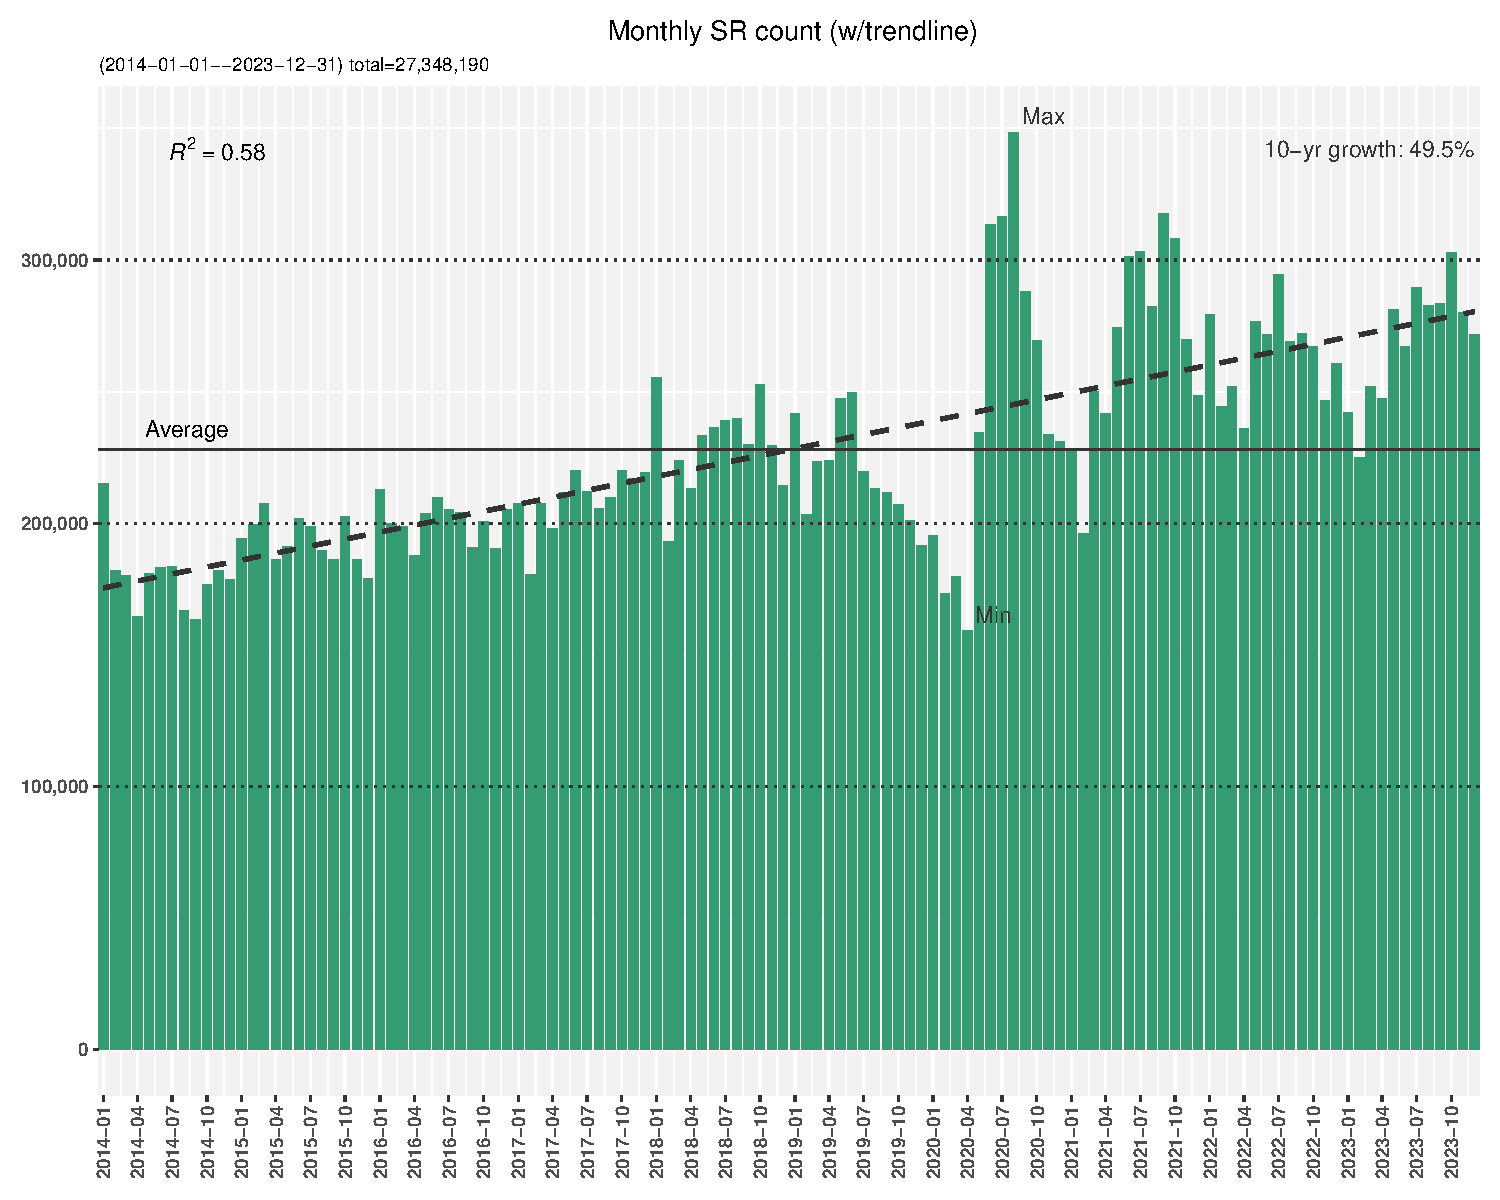
\includegraphics[width=\textwidth]{10-year-trend-monthly.pdf}
  \caption{10-year (2014-2023) Monthly SR Counts}
  \label{fig:10-yr-monthly}
\end{figure}

\begin{table}[tbp]
    \centering
    \normalsize
    \caption{Top 5 and Bottom 5 Days for SRs}
    \begin{tabular}{@{}lll lll@{}}
        \toprule
        \multicolumn{3}{c}{Top 5 Days} & \multicolumn{3}{c}{Bottom 5 Days} \\
        \cmidrule(r){1-3} \cmidrule(l){4-6}
        Date & Count & Rank & Date & Count & Rank \\
        \midrule
        2020-08-04 & 24,415 & 1 & 2014-12-25 & 2965 & 1 \\
        2020-08-05 & 19,560 & 2 & 2015-12-25 & 3247 & 2 \\
        2023-09-29 & 17,962 & 3 & 2014-04-20 & 3287 & 3 \\
        2020-07-05 & 16,916 & 4 & 2015-12-26 & 3405 & 4 \\
        2020-06-21 & 15,883 & 5 & 2016-11-06 & 3419 & 5 \\
        \bottomrule
    \end{tabular}
    \label{tab:top-10-counts}
\end{table}

This chart shows the 2-year period which is the basis for this analysis, by calendar month. 
Note that almost all the months before the COVID pandemic outbreak in Feb/Mar
of 2020 are ``below average'', while most of the months after that period are ``above average''. That level of higher usage
of the 311 system has continued into the early months of 2024. It is not surprising that the lowest SR counts-per-day occur during the Christmas holiday period. 

\begin{figure}[tbp]
  \centering
  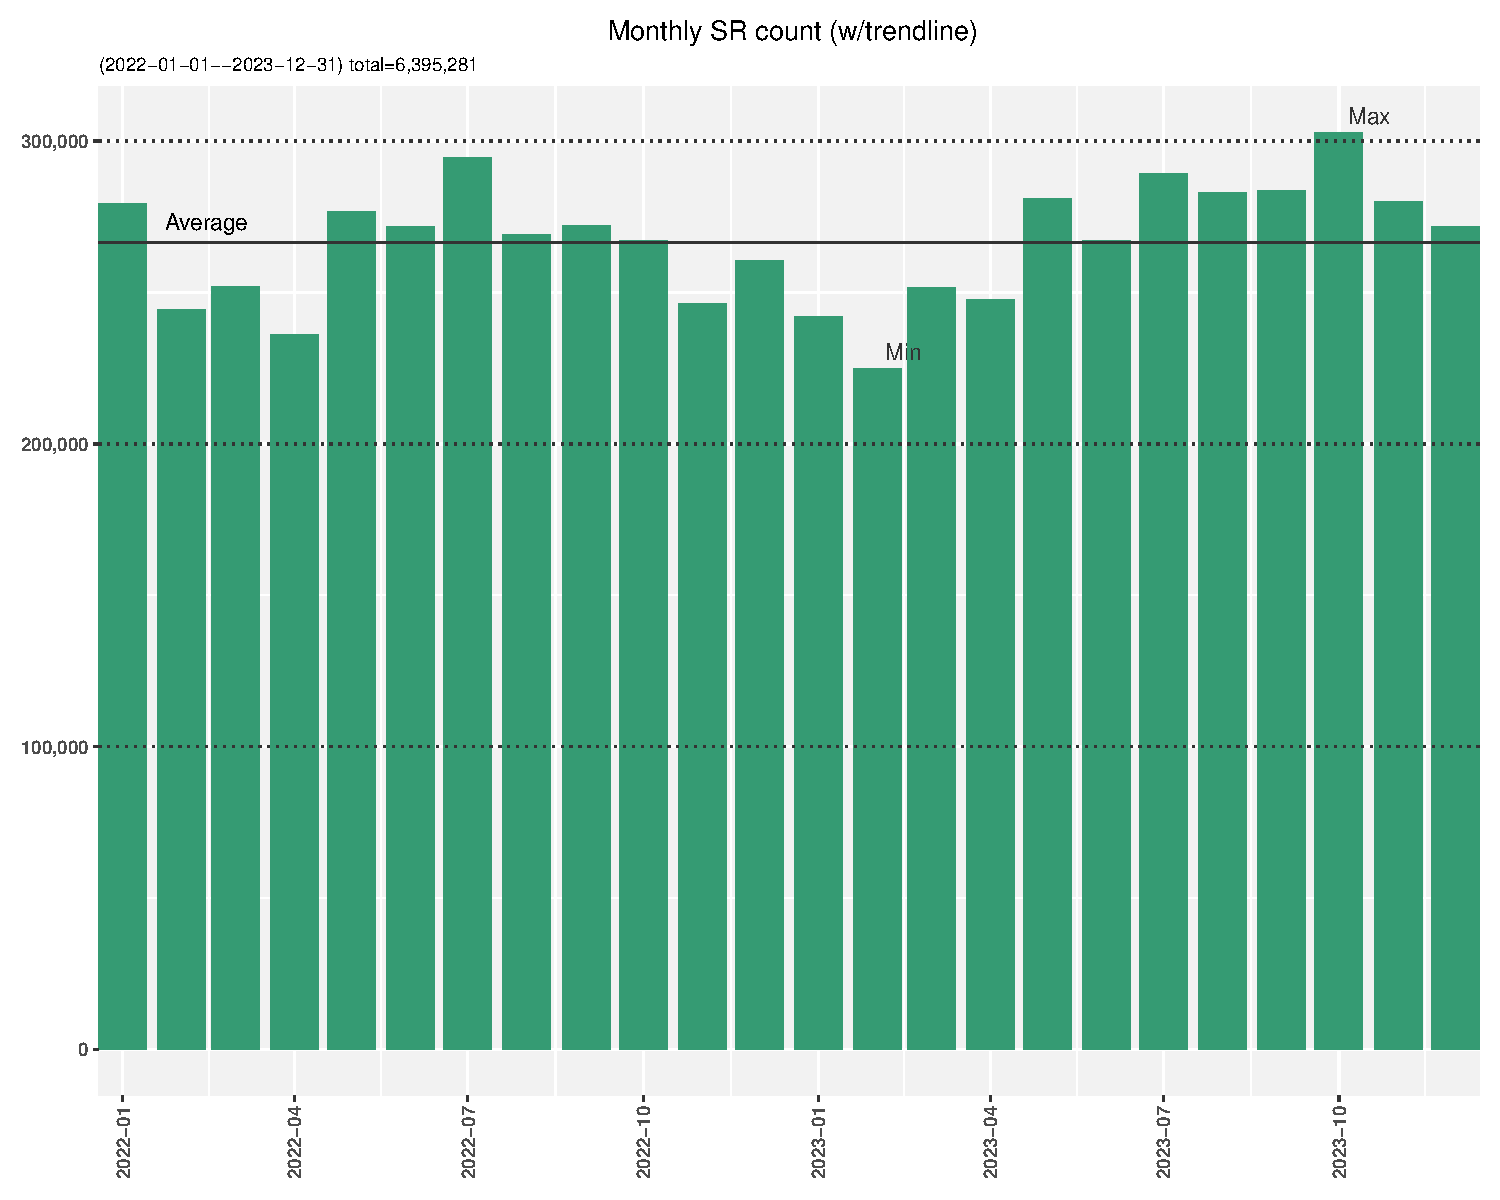
\includegraphics[width=\textwidth]{2-year-trend-monthly.pdf}
  \caption{Monthly SR Counts for 2022-2023}
  \label{fig:2-yr-monthly}
\end{figure}

Two important fields in this analysis effort are the responsible NYC Agency, and the type of complaint.
Given the size of the City of New York government, it is necessary to identify the responsible Agency as well as the type of complaint in order to 
identify the responsible party and assist in troubleshooting discrepancies.

When we discovered a data error, we typically observe one of two trends; either a single (or a few) Agencies are responsible (such as Dept of Transportation), 
or it is a system-wide issue that follows the general distribution of  SRs across the system. 
Thus we can often identify if it is an Agency specific problem, or a systemic issue.  (Note: a few key NYC Agencies are not 
represented in the 311 dataset. These include the New York City Housing Authority (NYCHA) and the
Department of Corrections (DOC).)

Although the 311 SRs involve 16 different agencies, there are the ``big six'' Agencies that comprise
90\% of the complaints. These six are (in order of \% of complaints):  

\begin{itemize}
	\item New York Police Department (NYPD)
	\item Housing Preservation \& Development (HPD
	\item New York City Department of Sanitation (DSNY)
	\item Department of Transportation (DOT)
	\item Department of Environmental Protection (DEP)
	\item Department of Parks \& Recreation (DPR)
\end{itemize}

\begin{figure}[tbp]
	\centering
	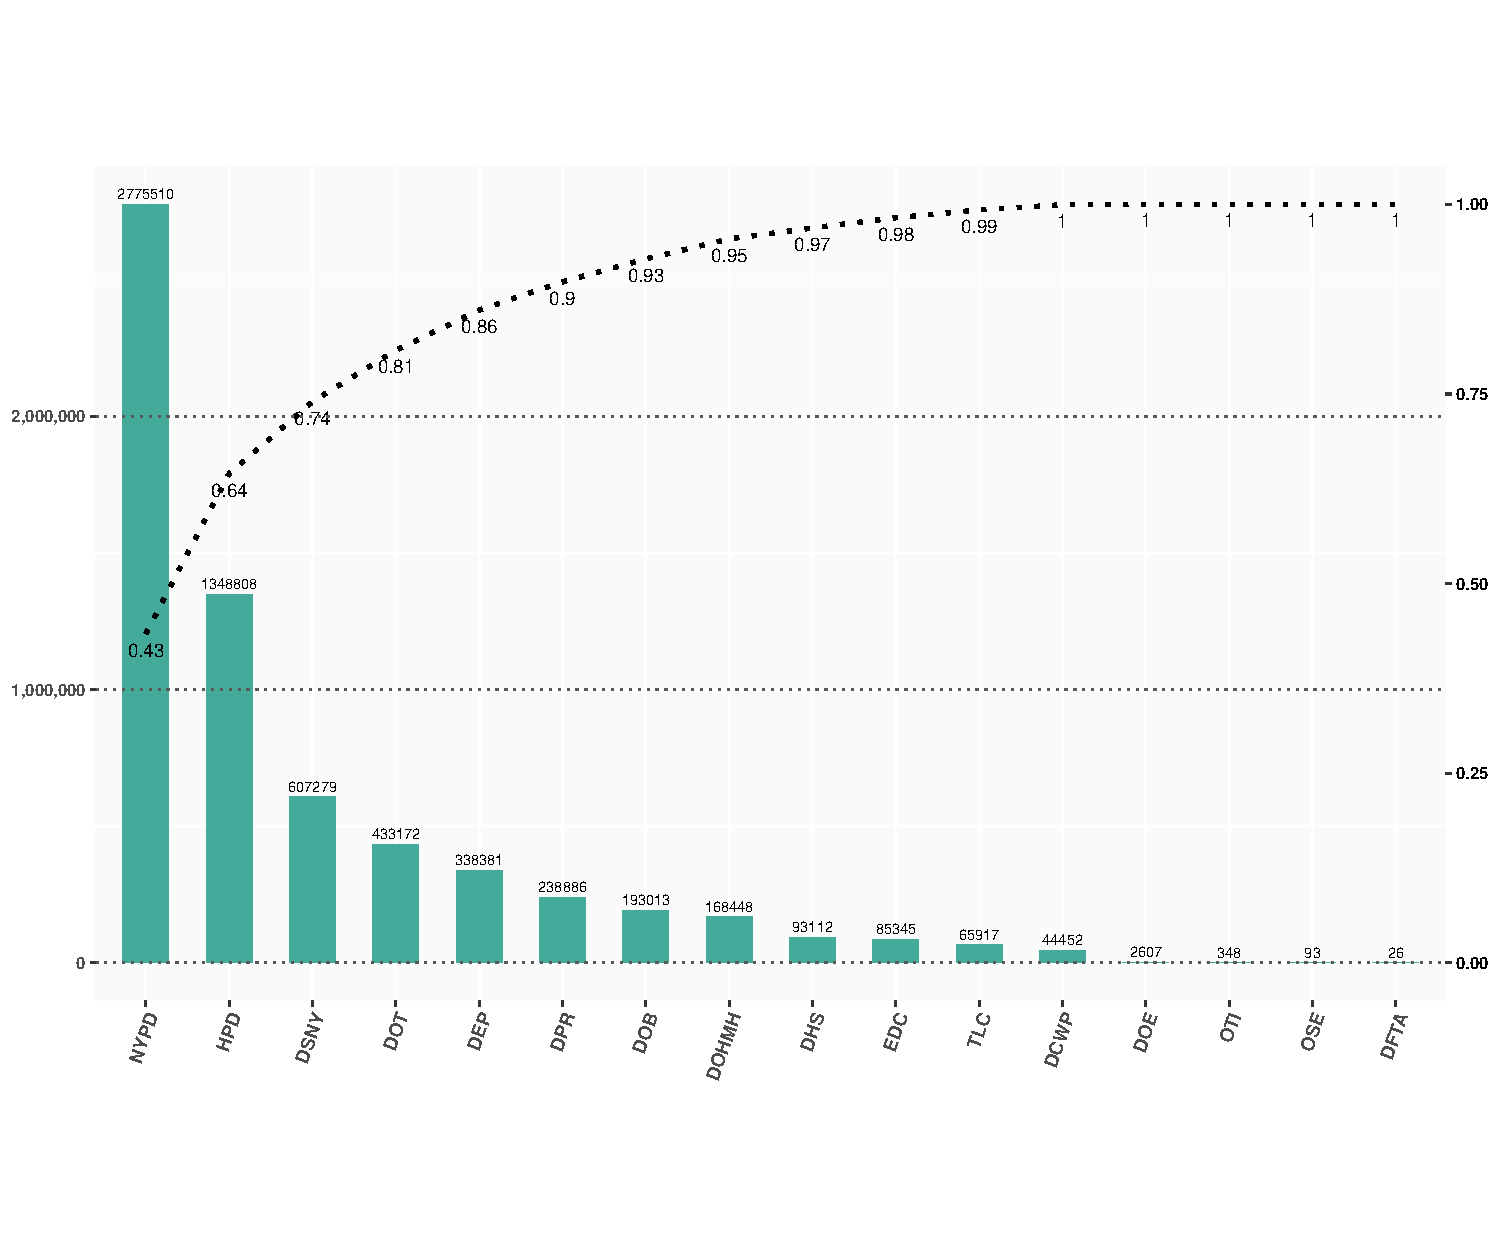
\includegraphics[width=\textwidth]{SRs_by_Agency.pdf}
  	\caption{SR counts by Agency with Cumulative Percentage}
	\label{fig:SRcountbyAgency}
\end{figure}

The distribution of complaint\_type skews to a few select complaints accompanied by a long tail.
This graph shows the top 20 complaint\_type(s) comprising 70\% out of a total of 220.

\begin{figure}[tbp]
  \centering
 	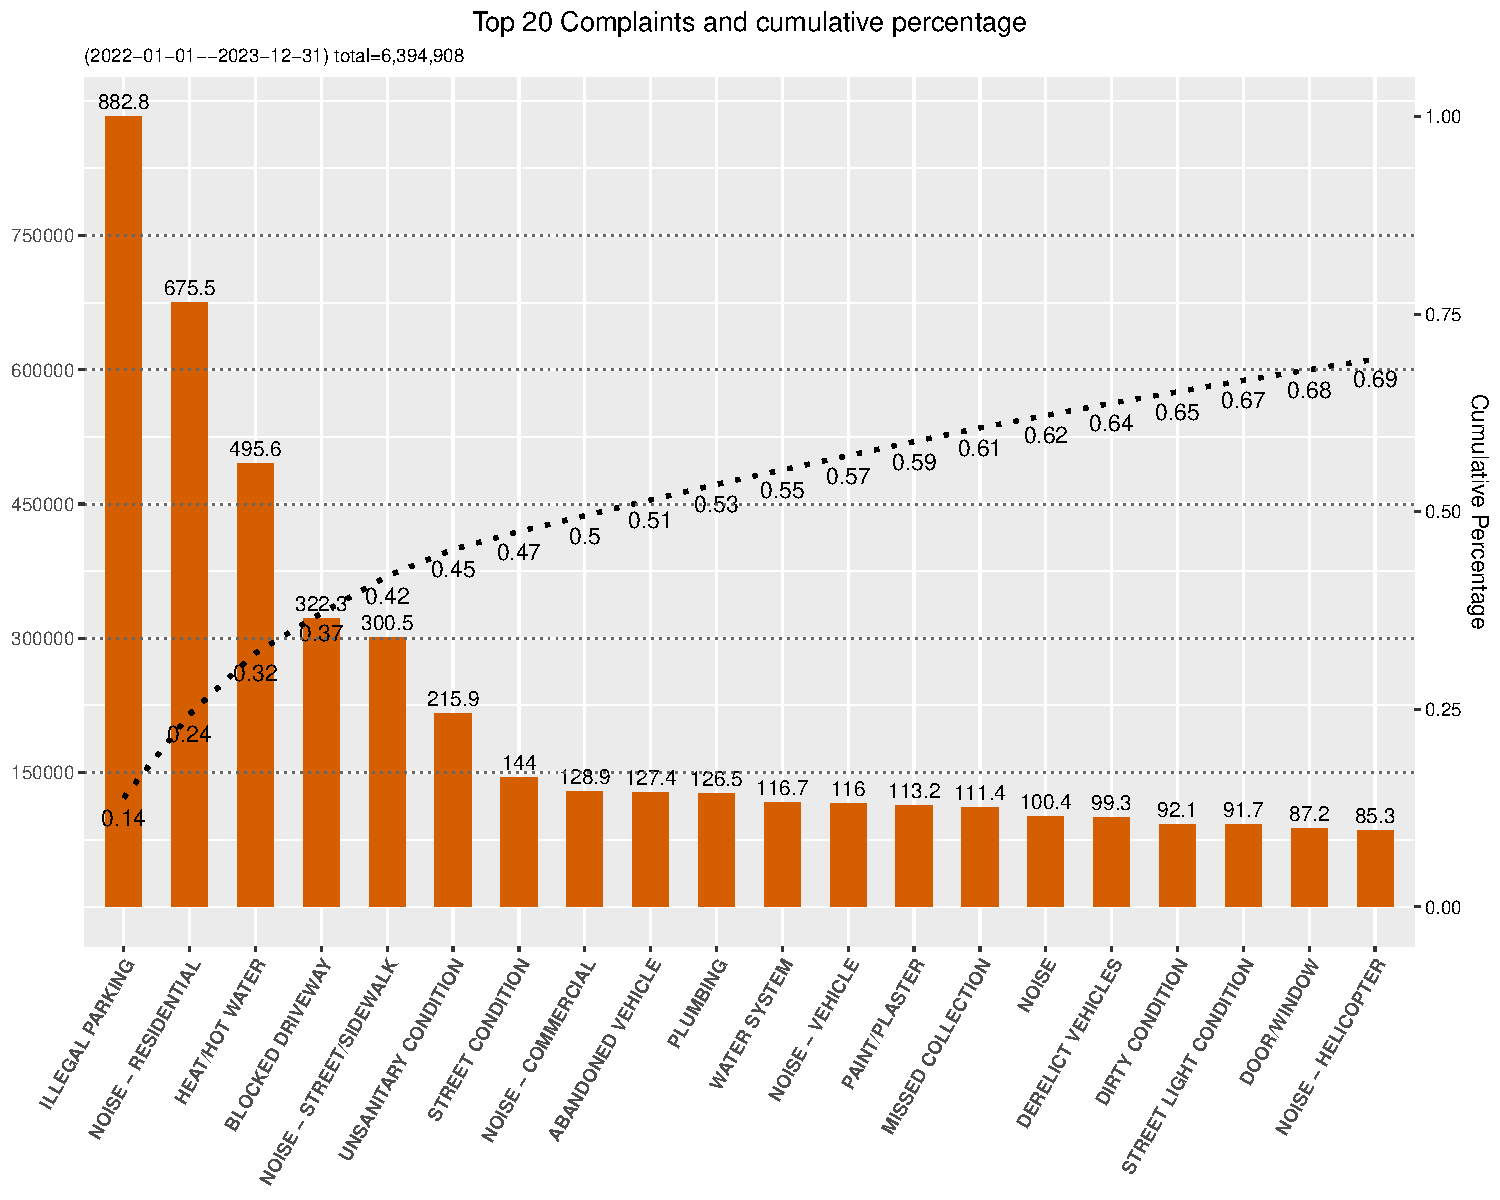
\includegraphics[width=\textwidth]{SR_by_Complaint_Type.pdf} 
	\caption{Top 20 complaint\_type(s) and Cumulative Percentage} 
	\label{fig:SR_complaints}
\end{figure}

The top 20 complaints contain several of the eight different types of ``Noise'' complaints (Residential, Commercial, Street, Helicopter, etc.). These Noise-related
complaints total 1.435 million in the 2022-2023 dataset, a full 22\% of all complaint types, which, when consolidated, is the most frequently occurring complaint\_type.
Illegal Parking is second, followed by Heat/Hot Water. Noise complaints are handled by NYPD, as is Illegal Parking and Blocked Driveway complaints, which contributes
significantly to the top ranking of the NYPD as the lead responsible Agency, receiving a full 43\% of all SRs. 
Housing, Preservation, \& Development are 2\textsuperscript{nd}, with 21\%

For  non-NYC residents, HPD is the City agency that manages the 177,569 NYC public housing units as well as monitoring
all City rental and leased apartment units. HPD collectively serves 528,105 people, a population larger than Atlanta or Miami. 
Hence the large number of Heat/Hot Water and Unsanitary complaints handled by HPD. 




\begin{table}[tbp]
    \centering
    \caption{Noise-related complaints\_type(s) by count with Agency}
    \normalsize
    \begin{tabular}{@{}lS[table-format=7.0,round-mode=places,round-precision=0]S[table-format=2.2,round-mode=places,round-precision=2]l@{}} % 'l' for left-aligned, 'S' for siunitx number alignment
        \toprule
        \textbf{complaint\_type} & \textbf{Count} & \textbf{Percentage} & \textbf{Agency} \\ 
        \midrule
        NOISE - RESIDENTIAL        & 675502 & 10.56 & NYPD  \\ 
        NOISE - STREET/SIDEWALK    & 300507 &  4.70 & NYPD  \\ 
        NOISE - COMMERCIAL         & 128892 &  2.02 & NYPD  \\ 
        NOISE - VEHICLE            & 115956 &  1.81 & NYPD  \\ 
        NOISE                      & 100413 &  1.57 & DEP   \\ 
        NOISE - HELICOPTER         &  85345 &  1.33 & EDC   \\ 
        NOISE - PARK               &  16620 &  0.26 & NYPD  \\ 
        NOISE - HOUSE OF WORSHIP   &   2757 &  0.04 & NYPD  \\ 
        \bottomrule
    \end{tabular}
    \label{tab:noisecomplaints}
\end{table}


There are also some curious and unusual Service Requests in the 311 data: 
tanning, tattooing, trans fat, unsanitary pigeon condition, illegal animal kept as pet, harboring bees/wasps, and the authors' favorite
radioactive material. New Yorkers certainly live interesting lives. 



\section{Data Cleansing Issues} \label{sec:issues}

What is data cleansing?  Wikipedia \href{https://en.wikipedia.org/wiki/Data_cleansing}{Data Cleansing} offers a good definition. 

``Data cleansing or data cleaning is the process of detecting and correcting (or removing) corrupt or inaccurate records from a record set, 
table, or database and refers to identifying incomplete, incorrect, inaccurate or irrelevant parts of the data 
and then replacing, modifying, or deleting the dirty or coarse data.''

Many quality criteria are required in order to process high-quality data. These include:

\begin{itemize}
	\item Data validation - this effort can span a number of criteria
	\begin{itemize}
		\item Mandatory fields: Certain data fields cannot be empty.
		\item Data-types: Certain fields must be of the correct type, e.g. numeric, character, date, 5 numeric digits, etc. Typically these are identified in a Data Dictionary.
		\item Domain adherence:  Many data fields must adhere to a specific domain of values, e.g. statuses, state names, zip codes, gender. This includes data
		fields that are restricted to certain ranges, such as longitudes and latitudes.
	\end{itemize}   
	\item Structural errors to include naming conventions, extra fields not in the Data Dictionary, or inconsistent data entry.
	For example intermixing blanks, spaces, NA, N/A, and \textless{}NA\textgreater{} all to indicate the absence of data.
	\item Redundant, unnecessary, or irrelevant fields
	\item Logical inconsistencies such as related fields that violate the nature of that relationship, e.g. a ``due date'' that is before the ``created date''
	\item Data standardization. Often free-form entry fields can suffer from inconsistent data structures. Efforts to standardize these fields can greatly assist analysis.
	\item Accuracy and precision, which of course are not the same thing 
\end{itemize}

This analysis effort is to identify the presence of such errors; not to correct them. That effort would be undertaken only after an investigation as to the why
and how such errors came about, and a discussion as to whether or not it is even an ``error''. Typically this requires discussions with subject matter experts (SMEs)
 and liaison within the various NYC Agency open data coordinators who can help identify the underlying cause for the error.
 For example, an invalid date field that is provided to the NYC Open Data data lake via an Agency integration could
be the result of selecting the wrong field from the source Agency's system, e.g. due\_date instead of closed\_date. In other cases, without a subject matter
expert, it is not possible to actually determine if the data is inaccurate or not. There are many empty values in the taxi\_company\_borough field. Are those
entries missing or does the entry in that field only apply to a very small number of complaint\_type(s) or circumstances. Only a SME
from the Taxi \& Limo Commission (TLC) can provide that answer. The R code used here to analyze the 311 Service Request dataset identifies
both obvious inaccuracies as well as potential errors requiring further investigation. It is not a conclusive list of errors, but rather mostly identifies
``a place to look'' for further evaluation and potential action.

This paper will focus on a set of specific data cleansing areas:

\begin{itemize}
	\item Examining structural issues within the data
	\item Validating data type correctness
	\item Identifying missing, blank, or N/A data
	\item Identifying invalid values
	\item Exposing logical inconsistencies \& inconsistent or unusual patterns in the data
	\item Accuracy and precision issues
	\item Identifying potential redundant or irrelevant data  
\end{itemize}



\section{Structural Issues}\label{sec:structural}

Structural issues in the context of data cleansing refers to issues related to the how data is organized, formatted, or structured within a dataset. Structural issues 
can make it difficult to analyze the data effectively. Some common structural concerns in this 311 SR 2022-2023 dataset include:

\begin{itemize}
	\item Data structure (data fields, columns, formats, data types, etc.) not corresponding to the Data Dictionary
	\item Verification of correct data types (numeric, character, geospactial, dates, etc.)
	\item Embedded or combined values: data elements that contain multiple pieces of information 
\end{itemize}

Here are some characteristics of the 311 SR data set:

\begin{itemize}
	\item There are 47 columns of data for each row, exportable as a CSV file.
	\item There are four date fields (created, closed, updated, due).
	\item There are three borough fields; two of which we believe to be duplicates.
	\item Two zip code fields, but not duplicates
	\item Seven street fields; one pair of which we believe to be duplicates
	\item Agency name and Agency abbreviation
	\item Two Police Precinct fields; not duplicates
	\item In addition to street/city, there are three other location fields: lat/long, NY State plane, and Block \#
	\item incident\_address and street\_name, e.g. incident\_address, 25 Grymes Hill Road and street\_name (Grymes Hill Road)
	\item One free-form text field, resolution\_description, which supports 934 characters of input, including commas and special characters
\end{itemize}


\textbf{Issue: Fields not in the Data Dictionary} The 311 SR \href{https://data.cityofnewyork.us/api/views/erm2-nwe9/files/b372b884-f86a-453b-ba16-1fe06ce9d212?download=true&filename=311_ServiceRequest_2010-Present_DataDictionary_Updated_2023.xlsx}{Data Dictionary}
 identifies 41 data columns (fields) along with related information for each column. 
 However, when you download the data or explore it via the online portal, you immediately note that there are 47 columns (fields).
 he additional six fields are not addressed in the Data Dictionary, but do and show up on the Column Manager widget
 as ``@computed\_region\_xxxx\_xxxx''. To some extent one can infer what the these @computed\_fields are, but it is not possible to know
for certain. These six fields are:

\begin{itemize}
	\item zip\_codes
	\item community\_districts
	\item borough\_boundaries
	\item city\_council\_districts
	\item police\_precincts
	\item police\_precinct 
\end{itemize}	

Here is a screenshot of the NYC Open Data Portal ``Column Manager'' page showing those columns:

\begin{figure}[tbp]
  \centering
 	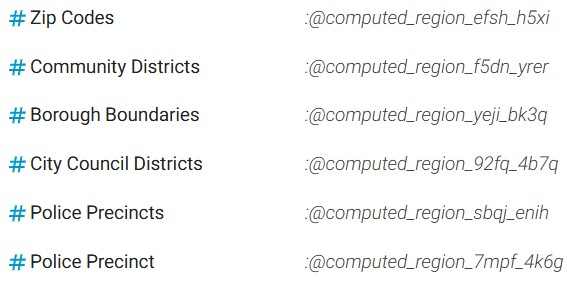
\includegraphics[width = .65\textwidth] {computed_fields_jpg.jpg}	
	\caption{Screenshot of Data Portal with ``@computed'' Columns}  
	\label{fig:computed-columns}
\end{figure}

This, of course, raises several questions:

\begin{itemize}
	\item How are these fields computed? Using what source data? Using what computational method?
	\item How can these fields be verified or cross-checked?
	\item Why are there two fields that appear redundant ``police\_precinct' and ``police\_precincts''? Are these redundant?
	\item What are ``borough boundaries''? They appear to be borough names. Why are they referred to as ``boundaries''?
	\item What are ``community districts''? Is this the same as the ``community\_board(s)'' that are part of the NYC government?
	\item Why are not these fields included in the official 311 SR Data Dictionary?
	\item Can these fields be reliably used for analytical purposes? 
\end{itemize}	

The last bullet point is the key here. Are these fields reliable and accurate, and can they be used for subsequent analysis? Unfortunately,
as of this date, those questions have not been fully addressed by the  NYC Open Data Team. This paper will further address that issue by
exploring the accuracy, validity, and candidacy for subsequent analytical usage.
	
	
	
\section{Validating data types}\label{sec:datatypes}
Fortunately, both the Data Dictionary and the portal column manager do a good job of indicating the data type.
As indicated by the red underline in Figure \ref{fig:computed-columns}, there is a small icon next to the field name 
which indicates the data type of the field. The stylized capital ``T'' indicates ``text'', the ``\#'' sign indicates 
``numeric'', a calendar icon indicates a ``date'' field, and the pin on a map symbol indicates a ``geospatial'' field. 
	
The following fields were checked for their specified data types:
	
\begin{itemize}
	\item created\_date, closed\_date, due\_date, and resolution\_action\_updated\_date: All are all in proper date format.
	\item zip\_codes and incident\_zip: All are 5 numeric digits except for 2 non-numeric entries for incident\_zip (``na'' and ``N/A'').
	\item x\_coordinate\_state\_plane \&  y\_coordinate\_state\_plane (a NY State geo-location system): All are all numeric.
	\item latitude \& longitude: Both are numeric.
	\item community\_districts, borough\_boundaries, city\_council\_district, police\_precinct, and police\_precincts: All are numeric.
	\item Free-form text fields that contain a ``,'' (e.g. incident\_address \& resolution\_description) are properly enclosed in quotation marks.
\end{itemize}	

All data fields were subjected to a test of ``correctness'' according to their ``type'' as specified
in the Data Dictionary. Of the nearly 300 million data fields to check (6.5 million rows, 47 fields per row), there were only two values that failed to test the
test for appropriate data type; those being two text entries in the incident\_zip field (``na'', and ``N/A''). All date fields were dates. All numbers were numeric.
All text fields were character. Data typing appears to not be an issue with this dataset.

 

\section{Blank \& N/A data}\label{sec:blanks}

Understanding the absence of data by field is an important factor when undertaking analysis. For example, if you wanted to see if the SRs were
closed before or after their due\_date, you would be challenged as 99.57\% of the due\_date field is blank. (Although with such a large dataset
that still leaves 24,411 values, all of which are ``N/A'. Which calls into question...are these missing values, or is the concept of a
due\_date simply not applicable for the vast majority of SRs?

When counting the various fields for blank or N/A values, the fields appear to divide into three groups: \textbf{Mostly Empty}, \textbf{Partially Empty}, 
and \textbf{Few/None Empty}. he Mostly Empty category ranges from 93-99.9\% blank. It includes such fields as taxi\_company due\_date, pickup\_location, and landmark. The Partially 
Empty includes such fields as location\_type, borough, and cross\_street. And the Few/None Empty includes created\_date, complaint\_type, agency, and status.
In some cases it may make sense to inquiry as to why some fields are frequently blank. Is the data difficult to capture? Does it pertain to only a small set
of complaint\_type(s) or Agencies? And if the data is truly that sparse, does it even make sense to collect it? Is it legacy data? For example, one would expect that every complaint\_type
that has a geographical component, such as an address, would also have a corresponding police\_precinct, community\_board, and community\_district since these
are all-inclusive throughout the five Boroughs of NYC. Addtionally, that it would have a lat/long. And generally that is the case, but these fields do have small number, but nonetheless significant, 
of empty entries. 

During the analysis, it was determined that the following fields are mandatory, and any row missing these fields should be removed from the dataset (which fortunately
very rarely occurred): created\_date, agency, complaint\_type, and unique\_key. The absence of any one of these four fields prohibits further analysis  as currently conducted. Again,
it is very rare occurrence, happening only 1-2 times in 6.4 million records. Here is a breakdown of bank and N/A entries by field.

\begin{table}[tbp]
\centering
\caption{Blank and N/A entries by Field}
\resizebox{0.8\linewidth}{!}{%
\normalsize
\begin{tabular}{lrrrl}
	\toprule
	\textbf{Field} & \textbf{Total Empty} & \textbf{Percent Empty} & \textbf{N/A Count} \\
	\midrule
		taxi\_company\_borough & 6391341 & 99.94 & 0 \\
		road\_ramp & 6379080 & 99.75 & 0 \\
		vehicle\_type & 6376266 & 99.71 & 0 \\
		due\_date & 6370497 & 99.62 & 6370497 \\
		bridge\_highway\_direction & 6367626 & 99.57 & 0 \\
		bridge\_highway\_name & 6340197 & 99.14 & 0 \\
		bridge\_highway\_segment & 6340190 & 99.14 & 0 \\
		taxi\_pick\_up\_location & 6329954 & 98.98 & 0 \\
		facility\_type & 5966588 & 93.30 & 0 \\
		landmark & 2635736 & 41.22 & 0 \\
		intersection\_street\_1 & 2143847 & 33.52 & 0 \\
		intersection\_street\_2 & 2140707 & 33.48 & 0 \\
		cross\_street\_1 & 1846594 & 28.88 & 0 \\
		cross\_street\_2 & 1846008 & 28.87 & 0 \\
		location\_type & 798775 & 12.49 & 0 \\
		bbl & 768109 & 12.01 & 0 \\
		city & 332086 & 5.19 & 0 \\
		street\_name & 280463 & 4.39 & 0 \\
		incident\_address & 280268 & 4.38 & 0 \\
		closed\_date & 248839 & 3.89 & 248839 \\
		resolution\_description & 132333 & 2.07 & 0 \\
		zip\_codes & 123167 & 1.93 & 0 \\
		borough\_boundaries & 101453 & 1.59 & 0 \\
		community\_districts & 101445 & 1.59 & 0 \\
		city\_council\_districts & 101445 & 1.59 & 0 \\
		police\_precincts & 101445 & 1.59 & 0 \\
		police\_precinct & 101416 & 1.59 & 0 \\
		latitude & 99778 & 1.56 & 0 \\
		longitude & 99778 & 1.56 & 0 \\
		location & 99778 & 1.56 & 0 \\
		x\_coordinate\_state\_plane & 99668 & 1.56 & 0 \\
		y\_coordinate\_state\_plane & 98822 & 1.55 & 0 \\
		resolution\_action\_updated\_date & 91399 & 1.43 & 91399 \\
		incident\_zip & 83220 & 1.30 & 2 \\
		descriptor & 74645 & 1.17 & 0 \\
		address\_type & 38655 & 0.60 & 0 \\
		unique\_key & 0 & 0.00 & 0 \\
		agency & 0 & 0.00 & 0 \\
		agency\_name & 0 & 0.00 & 0 \\
		complaint\_type & 0 & 0.00 & 0 \\
		status & 0 & 0.00 & 0 \\
		community\_board & 0 & 0.00 & 0 \\
		borough & 0 & 0.00 & 0 \\
		open\_data\_channel\_type & 0 & 0.00 & 0 \\
		park\_facility\_name & 0 & 0.00 & 0 \\
		park\_borough & 0 & 0.00 & 0 \\
		created\_date & 0 & 0.00 & 0 \\
	\bottomrule
\end{tabular}
}
\end{table}

%\FloatBarrier % Ensure all floats before this point are processed before moving on

Here is a graphic depiction of total empty (blank \& N/As) for each fields. You can see the natural grouping into the Most, Some, and Few categories
in the stair-type visualization. 

\begin{figure}[tbp]
  \centering
  	\caption{Number and Percentage of Empty/Blank Entries}
	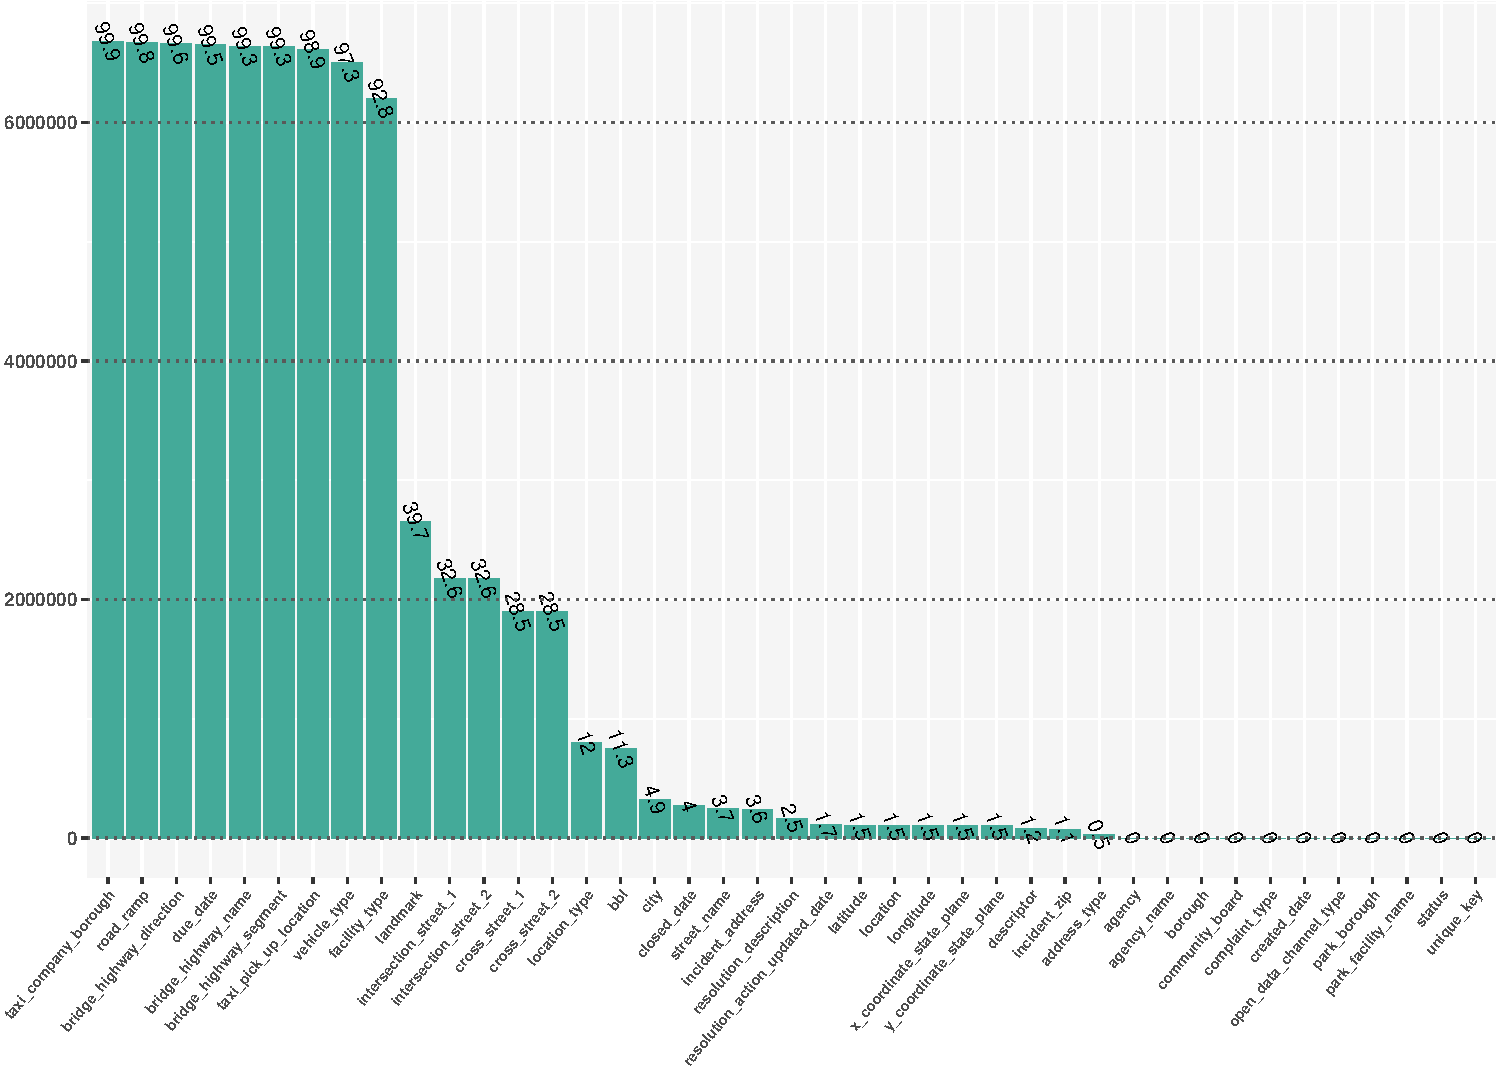
\includegraphics[width=\textwidth]{BlankFields.pdf}
	\label{fig:blank_fields}
\end{figure}



 \section{Validating Data for Acceptable Values}\label{sec:domain}
 While the dataset may have fields populated with data that appears correct, it is necessary to inspect those fields to determine if the data is indeed valid. 
 For example a date field that contains the value ``February 30, 2024'' is clearly not valid. Nor is a latitude of +95 deg north. 
 
 In this study, testing for invalid values revealed several serious issues associated with select fields. Accordingly, an analyst would need to be
extra diligent if using these fields for analysis. In all likelihood, rows with invalid field values would  need to be removed from the
dataset before conduction further analysis. Here are some results.

\begin{itemize}
	\item Latitude and Longitude fields were tested to ensure all fell within the geographic boundaries of the City of New York. All did.
	\item The unique\_key field was in fact unique.
	\item Many fields have a domain of acceptable values. Often these values are determined from common usage or by examining
	larger historical datasets. Unfortunately, these domains of acceptable values are not specified in the Data Dictionary. These fields all tested as
	compliant within their domain of acceptable values as determined by examining a 10-year dataset:
		\begin{itemize}
			\item address\_type
			\item status
			\item borough, borough\_boundaries, \& park\_borough 
			\item data\_channel
			\item vehicle\_type
			\item city\_council\_district
		\end{itemize}
\end{itemize}	

	\subsection{Issues with Zip Codes}
	\label{sec:zipcodesissues}
	 Unfortunately some fields proved to be  problematic when comparing the values to a domain of legal values.
	 For example, all zip codes (two fields: zip\_codes and incident\_zip) should be valid as defined by the USPS database
	 which contains 37,946 valid zip codes.
	 
	The computed field zip\_codes proved especially problematic with 58\% (3.6 million) of the field entries being invalid.
	That high number indicates that the computation of this field is highly inaccurate. We recommend
	dropping this field for future analytic efforts.
	
	Furthermore, the field incident\_zip while having only .07\% invalid entries, still is a problem with 4163 such errors.
	As the zip code is a primary measure of many NYC city services, 
	and with a freely available database for which to validate entries, it seems an oversight 
	that any such errors could creep into the 311 system. Some invalid entries can  
	clearly be identified as incorrect just by observation, e.g. 10000, 12345, 11111, etc. 
	
	The breakdown of the invalid entries in the zip\_code, sorted by Agency shows that the distribution by percentage
	almost precisely mirrors the overall breakdown of SRs by Agency as shown in . This indicates a systemic problem, and since the
	zip\_code fields is one of the computed fields, it appears these errors are caused by incorrect computations rather
	than by any Agency mistake.
	
	The  errors in the incident\_zip field are more troubling, even though they are, percentage-wise, small. Here is a graphic 
	illustrating how these errors occur by Agency. Here we can see that the majority of these errors lie in the Dept of Transportation,
	NYPD, Taxi \& Limo Commission (TLC), and the Economic Development Council (EDC) among others. This representation
	does not follow the full SR distribution indicating that these errors are likely generated by an incorrect
	process or application residing at those particular Agencies; it is not a systemic problem.

	\begin{figure}[tbp]
		\centering
		\caption{Invalid incident\_zip(s) by Agency}
		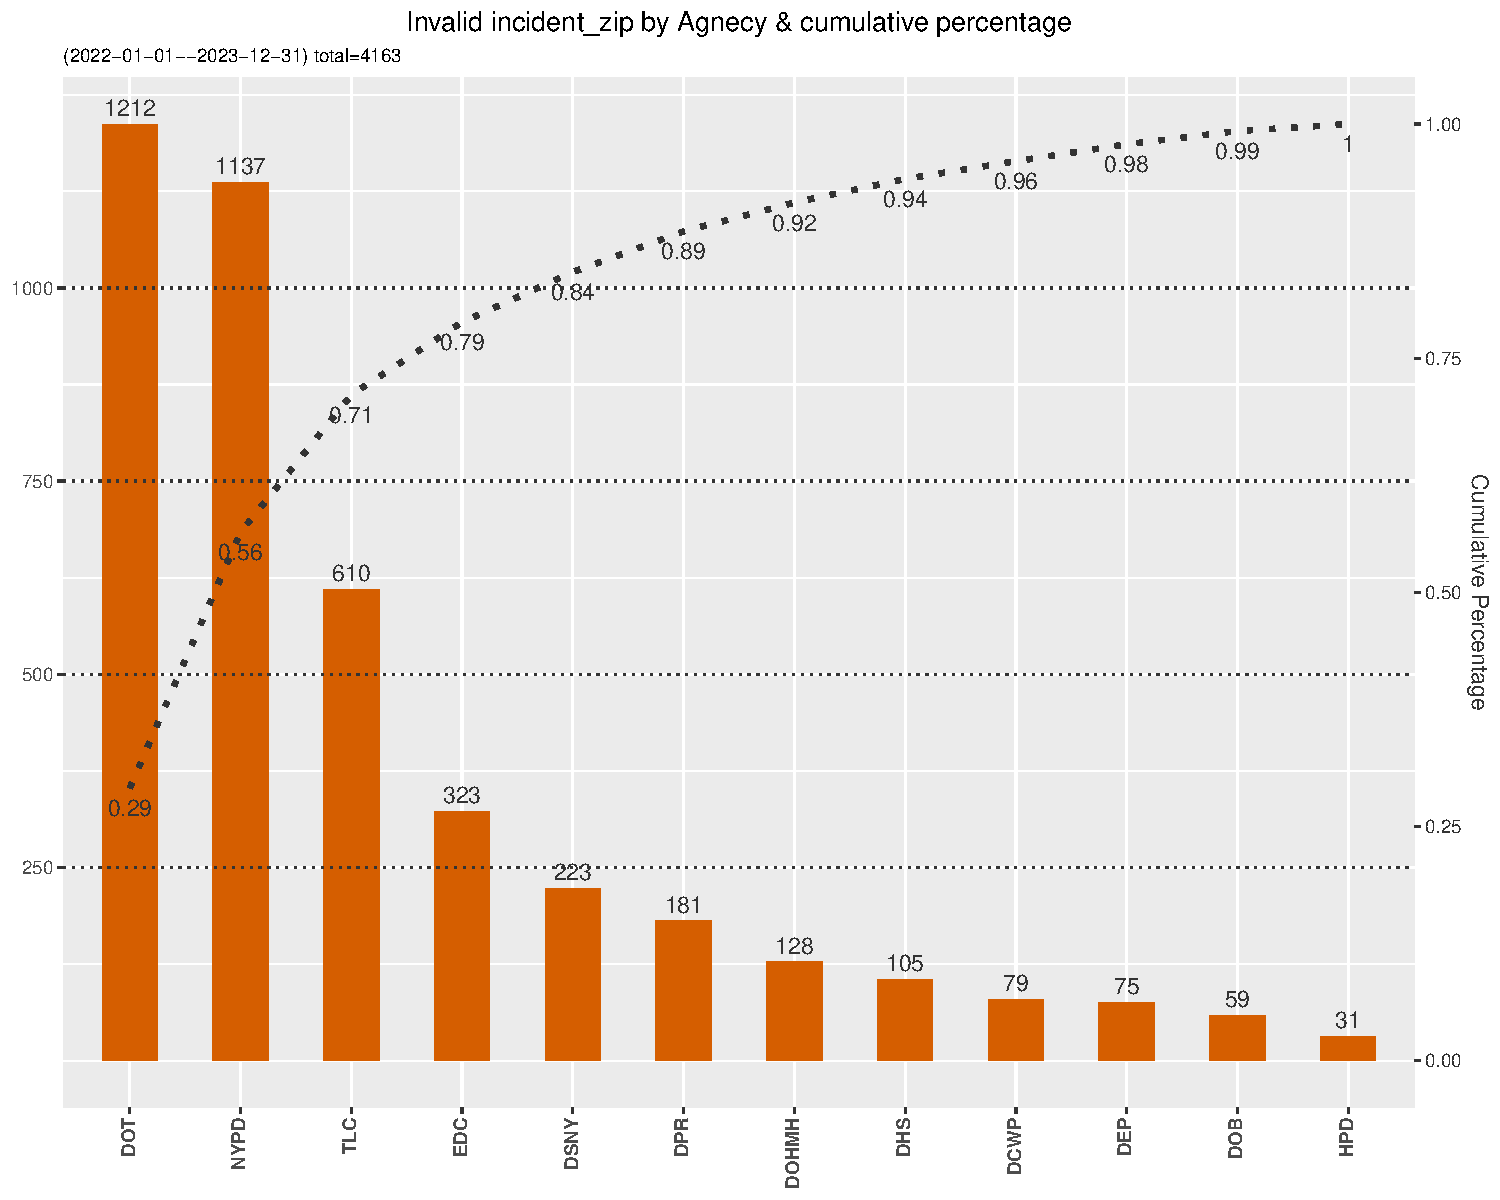
\includegraphics[width=\textwidth]{invalid_incident_zip.pdf} 
		\label{fig:invalid_incident_zip}
	\end{figure}
	
		\subsubsection{Case Study: Noise Complaints by Zip Code}{label{sec:case-study-zip-codes}
		\textbf{Scenario:} The NYC Office of Nightlife (ONL) wants to know ``What are the top 10 zip codes for Noise Complaints (all 8 types) over the last two years?''
		The goal is to assess the impact of the recent NYC effort looking to promote a safe and vibrant nightlife scene in NYC while seeking to ease
		strained relations between bar and club owners. 
		
		It may come as a surprise to non-NYC residents that dancing at bars and restaurants has been illegal since 1926 (during prohibition), and was only just repealed in 2018. 
		
		On the surface this would seem like a simple effort.  The NYC Open Data Portal allows for selection of a timeframe (2022-2023), complaint-type
		begins with ``Noise'', and group by Zip code, sorted descending by count.  You can do this analysis and grouping right inside the NYC Open Data Portal. \textit{Voila!}

		However, this analysis uses the zip\_codes field, one of the (six) computed fields that has shown to have validity problems. If we repeat the analysis with the 
		incident\_zip field instead of the zip\_codes field, we obtain a different set of zip code results:
		
		Let's subject these two data sets to validation against the US Postal Service zip code database.
	 
\begin{table}[tbp]
    \centering
    \normalsize
    \caption{Comparison of Top Ten Zip Codes Lists}
    \begin{tabular}{@{}lS[table-format=6.0,round-mode=places,round-precision=0]c@{\hskip 0.5cm}@{}lS[table-format=6.0,round-mode=places,round-precision=0]c@{}}
        \toprule
        \multicolumn{3}{c}{\textbf{zip\_codes}} & \multicolumn{3}{c}{\textbf{incident\_zip}} \\
        \cmidrule(r){1-3} \cmidrule(l){4-6}
        \textbf{Zip Code} & \textbf{Count} & \textbf{Valid?} & \textbf{Zip Code} & \textbf{Count} & \textbf{Valid?} \\
        \midrule
        11275 & 104556 & FALSE & 10466 & 104562 & TRUE \\
        12420 & 27503 & TRUE & 10023 & 27972 & TRUE \\
        12428 & 26564 & TRUE & 10031 & 25548 & TRUE \\
        10935 & 25508 & FALSE & 10457 & 25066 & TRUE \\
        10934 & 23448 & FALSE & 10453 & 24752 & TRUE \\
        10931 & 22381 & TRUE & 10456 & 24751 & TRUE \\
        10930 & 22121 & TRUE & 10452 & 22527 & TRUE \\
        17613 & 21963 & FALSE & 10025 & 21705 & TRUE \\
        10936 & 21707 & FALSE & 10458 & 21689 & TRUE \\
        11606 & 21435 & FALSE & 10032 & 20622 & TRUE \\
        \bottomrule
    \end{tabular}
    \label{tab:zipcodes}
\end{table}

	As indicated, six out of ten zip\_codes are invalid, which corresponds closely with what is observed in the overall dataset (58\%). Whereas the incident\_zip
	field is completely valid, again in-line with the overall incident\_zip validation percentage (99.04\%). If the analysis performed using the zip\_codes field were to be
	presented to the Director, ONL, the conclusion would be in error. Perhaps more curious than the differing zip codes on the two lists, 
	is the fact that the numerical counts are nearly identical;  the overall counts are quite close. This is curious since
	one field is computed while the other is via data entry; the computed protocol is again the suspect. The algorithm appears to be counting corrrectly (or nearly so)
	but mis-identifying the corresponding zip code.

	
	\subsection{Issues with Police Precincts}
	\label{sec:police-precincts}
	A curious case also exists when examining the two nearly identical fields - police\_precincts and police\_precinct. Both of those fields are among
	the ``computed'' fields in the dataset. 
	Using \href{https://www.nyc.gov/site/nypd/bureaus/patrol/precincts-landing.page}{NYPD Precinct listings} it's possible to determine the valid
	police precincts; they are generally numeric or have numeric representations in the dataset. 
	
	However, what we find is that both fields police\_precinct and police\_precincts  have  35\% invalid entries.
	Unfortunately, they're not the same invalid entries. 
	
	For the police\_precincts field, there are 2,171,864 invalid entries (35\%)., a consequential number of errors. Similarly for the police\_precinct field,
	 there are 2,171,778 invalid entries ( also 35\%), however they are not the same counts for the two similar fields.

	The top ten (by count) of invalid precincts for each field are:

	\begin{table}[tbp]
	\normalsize
	\centering
	\caption{Comparison of the fields police\_precinct and police\_precincts}
		\begin{tabular}{ccccc}
		\toprule
		\textbf{Invalid Precinct} & \textbf{police\_precinct count} & \textbf{police\_precincts count} & \textbf{Delta}\\
		\midrule
			62 & 151808 & 151720 & 88 \\
			72 & 148881 & 148796 & 85 \\
			67 & 133171 & 133115 & 56 \\
			64 & 111236 & 111221 & 15 \\
			60 & 105252 & 105317 & -65 \\
			65 & 103334 & 103306 & 28 \\
			53 & 100097 & 100074 & 23 \\
			73 & 97746 & 97755 & -9 \\
			68 & 94204 & 94254 & -50 \\
			66 & 93654 & 93848 & -194 \\
	\bottomrule
	\end{tabular}
	\label{tab:comparison-precincts-diff}
	\end{table}
	
	A graphic representation of the invalid police\_precincts plotted by Agency show a near perfect match to the
	distribution of the entire 6.4 million SRs as seen in Figure \ref{fig:SR_counts_by_Agency}. Note that the ``big six'' Agencies account for 90\% of these invalid precinct errors, identical
	to the overall distribution of all SRs. (The same is true for a similar graph of by the police\_precint field.) This strongly suggests that this is a systemic problem, almost certainly caused by the computation method applied for these two fields.
	 
	\begin{figure}[tbp]
	  \centering
	  \caption{Invalid NYPD precincts by Agency}
	  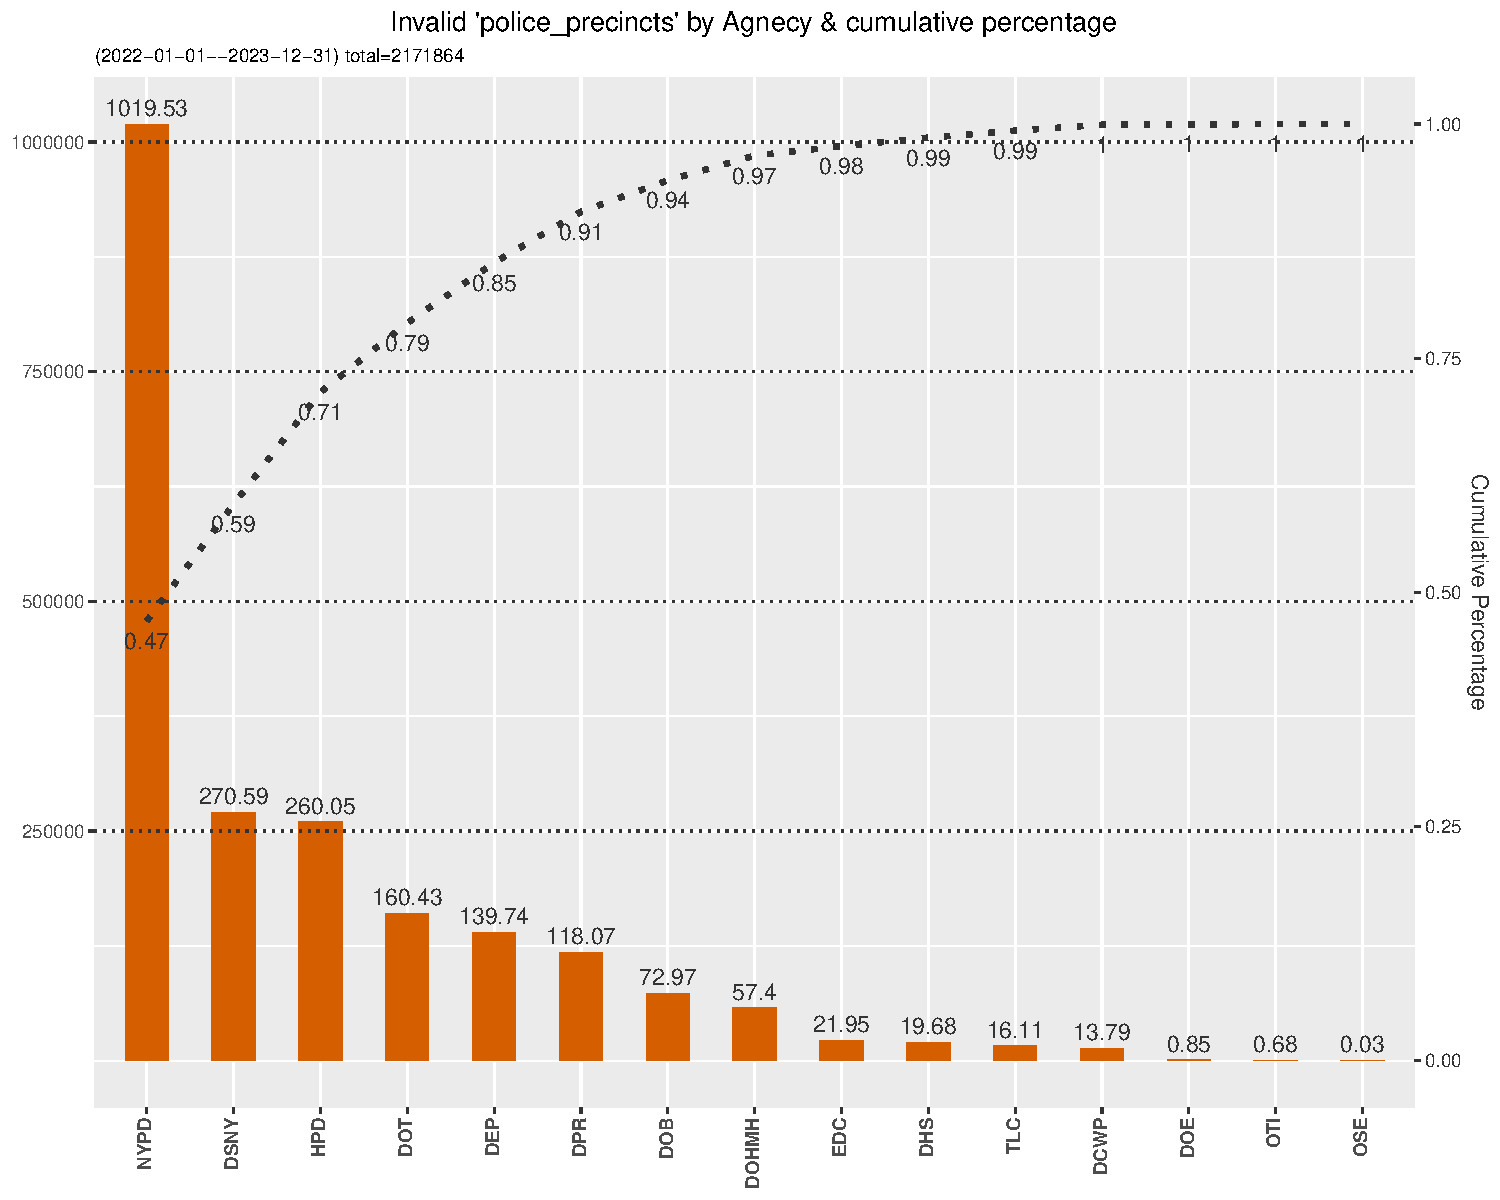
\includegraphics[width=\textwidth]{invalid_police_precincts.pdf}	  
	  \label{fig:invalid_police_precincts_zip}
	\end{figure}

	\subsection{Issues with Community Boards}
	Community Boards are an important aspect of NYC government. They are the most local, grassroots form of City government, 
	and a vital connection between communities and elected officials and City agencies. They are organized by the five Boroughs of NYC and represented
	in this dataset as ``\#\#-Borough'', e.g. ``10 Bronx'' and report to the various Borough Presidents in NYC. As such, they play an important role in the quality of life for all New Yorkers.
	There are 59 community boards throughout the City: 12 Community Districts in the Bronx, 18 in Brooklyn, 12 in Manhattan, 14 in Queens and 3 in Staten Island.
	The Community Boards are used frequently as a way to measure distribution of City services throughout the five boroughs, so correctness is important. 
	NYC Borough Presidents in particular are focused on the services offered at the Community Board level within their respective Borough.
	
	In the 2022-2023 dataset there are 27,276 invalid community\_board entries which represents 0.43\% of non-blank data. 
	There are a total of 12 different invalid community boards, to include: 
	
		\begin{table}[tbp]
		\centering
		\caption{Top Ten Invalid 'community\_board' Values}
		\normalsize
		\begin{tabular}{rlr}
		\toprule
		\textbf{Rank} & \textbf{Invalid CB} & \textbf{Count} \\
			\midrule
				1 & 64 MANHATTAN & 7144 \\
				2 & 83 QUEENS & 5133 \\
				3 & 55 BROOKLYN & 3327 \\
				4 & 81 QUEENS & 3180 \\
				5 & 80 QUEENS & 2407 \\
				6 & 26 BRONX & 2364 \\
				7 & 28 BRONX & 1128 \\
				8 & 82 QUEENS & 1054 \\
				9 & 95 STATEN ISLAND & 515 \\
				10 & 27 BRONX & 514 \\
			\bottomrule
		\end{tabular}
		\end{table}
		
		The distribution of invalid Community Boards by Agency is not consistent with the overall SR Agency distribution. This indicates that there are likely
		specific issues at some key Agencies, in this case Taxi \& Limo Commission (TLC), Parks \& Recreation, etc. It's not a large error, but the division of services
		(and complaints) by Community Board is a well-tracked measure so accuracy is again important.

		\begin{figure}[tbp]
	 	 \centering
		  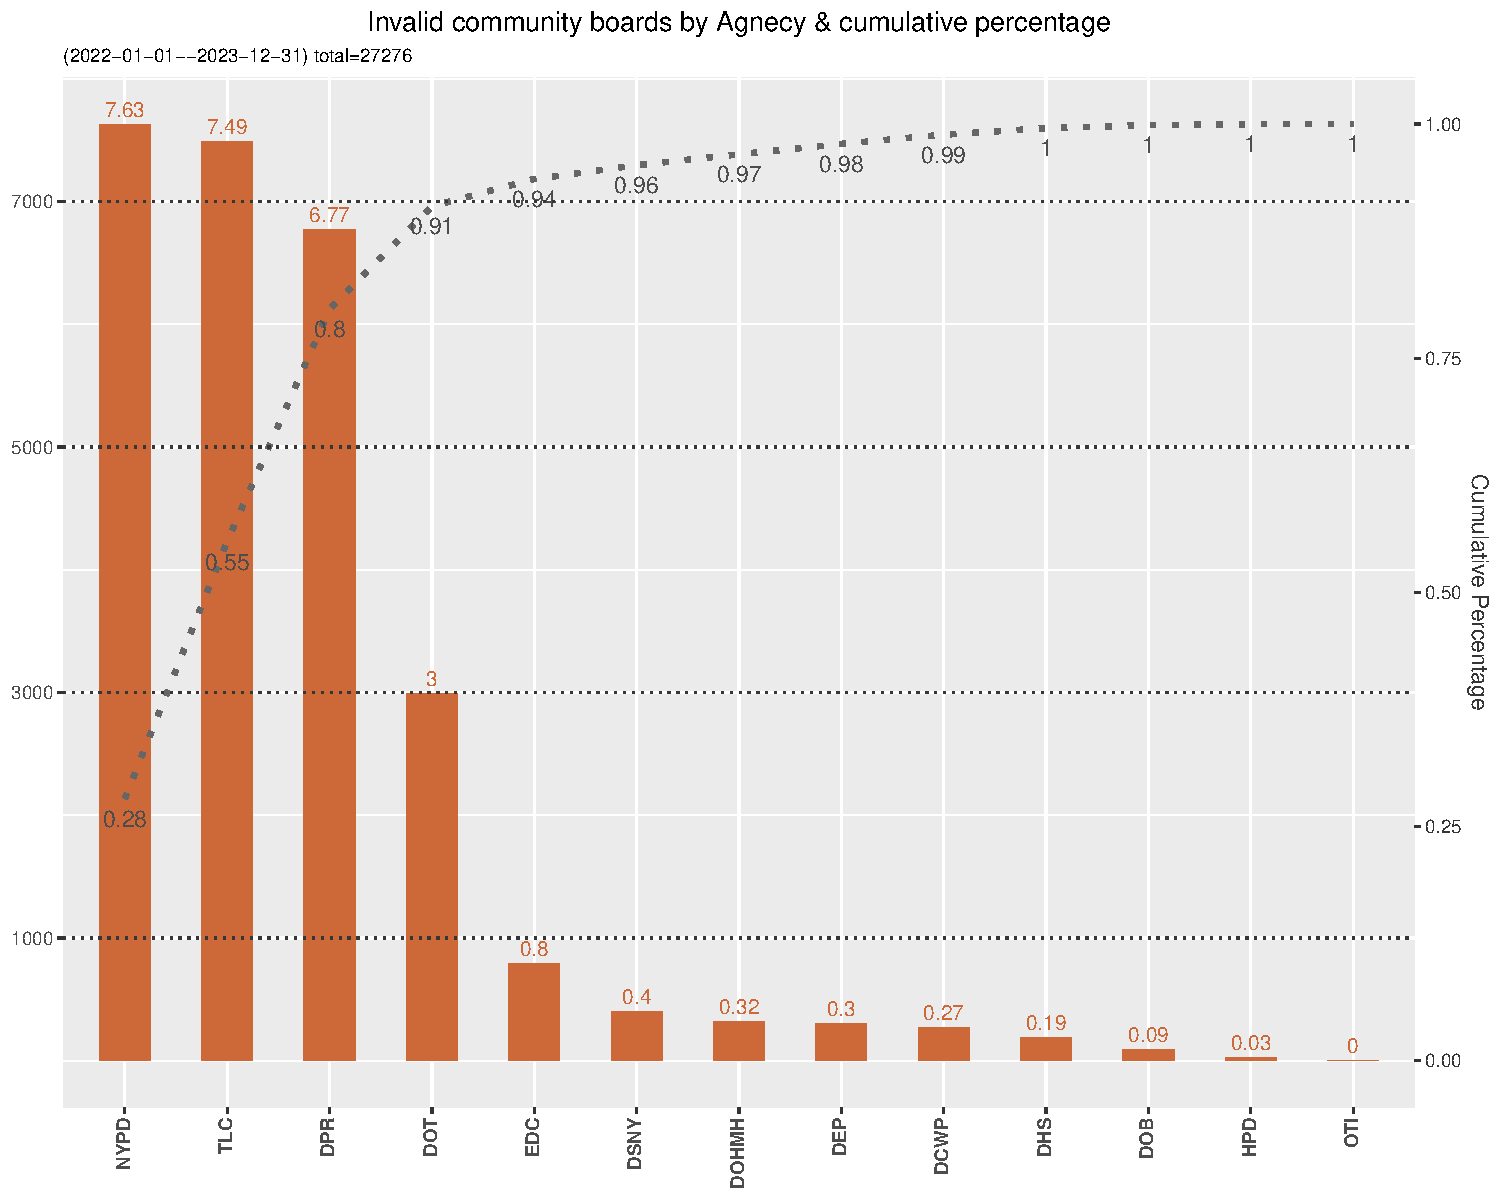
\includegraphics[width = \textwidth]{invalid_community_boards.pdf}
		  \caption{Invalid Community Board by Agency}
		  \label{fig:invalid_community_boards}
		\end{figure}


	\subsection{Issues with Community Districts}
	Another of the computed fields is community\_districts. Community Districts are the boundaries for the Community Boards, but unlike how Community Boards are
	an arm of the government of New York City, the Community District is used by the Department of City Planning (DCP) for purposes of environmental, socio-economic, and
	demographic purposes. DCP is the NYC''s primary land use agency and is instrumental in the City's physical framework.  It is a geographical division rather
	than a local government division. And like Community Boards, the Community Districts are frequently cited as a means to track zoning, housing, community facilities,
	and waterfront/open/public spaces. It is another of the NYC well-tracked measures.

	Due to how the community\_district data is formatted, it is not possible to establish validity. However, it is possible to determine that the dataset contains
	72 unique entries, while there are only 59 valid Community Districts. So it would appear that there are 13 invalid community\_board(s) contained in the dataset.
	
As previously mentioned, the dataset has four data fields:  created\_date, closed\_date, due\_date, and resolution\_action\_update\_date.
The due\_date field has few entries to analyze; 99.62\% of due\_date entries are ``N/A''.  It is not known if the due\_date(s) are truely
``not applicable'' or that the due\_date field is rarely used. The  resolution\_action\_update\_date field serves as a date-time marker
showing when the SR record was last updated.  All the date fields are recorded to the second, e/g/ ``2022-02-11 13:43:05''.

\subsection{created\_date and closed\_date(s) -- Negative Duration}
Let's look first at the created\_date and closed\_date fields. You might expect that these two fields are automatically populated by the 
SR application software, either the software used at the 311 organization or that used at the Agencies that are integrated with the 311 system;
and typically that is indeed the case. In such a case, the act of creating an SR would automatically trigger an entry in created\_date based on a system-wide clock. Thus
the created\_date is associated with setting an SR status to ``new'' or ``open''. And similarly when an SR's status is changed to
``closed'' then the closed\_date would be populated. 

Unfortunately, our analysis found that that assumption is not always the case. When you analyze the various date fields, several
anomalies become quickly apparent:

	\begin{itemize}
		    \item Some SRs have a closed\_date that occurs before the created\_date.
		    \item Some created\_date(s) and closed\_date(s) appear either in the future or in the far distant past.
		    \item There are a large number of SRs that are closed and created exactly at midnight or exactly at noon. 
	\end{itemize}

\textbf{Why are these date fields important?} They're important because citizens, NYC Government Officials, and NYC Agencies use these dates
to measure the responsiveness for providing the services. How long does it take to replace an out-of-order street light?
How rapid is the response to a report of domestic violence? Does the NYPD response to a noise complaint in Staten Island take
longer than in Manhattan? How long does it take to repair a street pothole in Queens? 

The measure of ``duration'', of the response time of a 311 call is a closely watched, carefully scrutinized metric, 
both in terms of overall performance and with a geographical area. And it can have broad political, organizational,
and budgetary consequences. Duration is not a field in the dataset, but it is easily computed by closed\_date - created\_date.
Let's look at some anomalies in this ``duration'' field.

Closed-before-Created:  There are 12,251 SRs that are closed before they were created, thereby generating a nonsensical 
``negative duration''. While this is a small percentage overall (0.2\%) it can have significant impact on response time analysis.
In most cases, these ``negative durations'' appear to just be mistakes. Here is a sample of some of the largest and the
smallest errors:

\begin{table}[tbp]
    \centering
    \caption{Largest and Smallest errors (days)}
    \normalsize
    \begin{tabular}{>{\ttfamily}l l l r l}
        \toprule
        \multicolumn{5}{c}{\textbf{Largest errors (days) excluding extreme negative values}} \\
        \midrule
        \textbf{created\_date} & \textbf{closed\_date} & \textbf{duration} & \textbf{agency} \\
	        \midrule
	        2023-01-27 14:40:00 & 2022-01-14 14:40:00 & -378.0 & DOT \\
	        2023-01-18 10:06:00 & 2022-01-12 10:06:00 & -371.0 & DOT \\
	        2023-01-27 14:36:00 & 2022-01-22 14:35:00 & -370.0 & DOT \\
	        2023-01-11 11:10:00 & 2022-01-09 11:10:00 & -367.0 & DOT \\
	        2023-12-18 03:13:00 & 2023-01-16 13:10:00 & -335.6 & DOT \\
	        \midrule
	        \multicolumn{5}{c}{\textbf{Smallest errors (days)}} \\
	        \midrule
	        \textbf{created\_date} & \textbf{closed\_date} & \textbf{duration} & \textbf{agency} \\
	        \midrule
	        2023-06-28 07:07:31 & 2023-06-28 07:07:00 & -0.00036 & DOT \\
	        2023-06-29 09:10:20 & 2023-06-29 09:10:00 & -0.00023 & DOT \\
	        2023-01-12 06:50:13 & 2023-01-12 06:50:00 & -0.00015 & DOT \\
	        2023-06-26 08:09:07 & 2023-06-26 08:09:00 & -0.00008 & DOT \\
	        2023-01-12 06:51:01 & 2023-01-12 06:51:00 & -0.00001 & DOT \\
	        \bottomrule
    \end{tabular}
    \label{tab:combined_errors}
\end{table}

The largest errors are shown ``excluding extreme negative values''. We found eight SRs with extremely large negative durations (\textless{} -730),
all containing an entry of ``1900-01-01'' as the closed\_date, which generates extremely large negative durations exceeding 44,601 days (122 yrs).
That large of an anomaly can skew statistical results, even though the number of occurrences is small. This is especially curious
as the date ``1900-01-01'' is also the earliest date that Microsoft Excel can accommodate as well as how Excel treats a blank
cell that is designated as a date. All raising suspicions that perhaps these dates were imported into the 311 system from Excel.

According, these  SR rows are removed from the box \& whiskers plot. Note that these extremely large negative duration SRs all
are from the Department of Homeland Services (DHS) Sample: 

\begin{table}[tbp]
    \centering
    \caption{Sample of SRs with extremely large negative durations}
    \normalsize
    \begin{tabular}{l l r l}
        \toprule
        \textbf{created\_date} & \textbf{closed\_date} & \textbf{duration} & \textbf{agency} \\
	        \midrule
	        2022-02-11 13:43:05 & 1900-01-01 & -44602 & DHS \\
	        2022-02-11 11:03:38 & 1900-01-01 & -44602 & DHS \\
	        2022-02-11 08:29:49 & 1900-01-01 & -44601 & DHS \\
	        2022-02-11 14:08:08 & 1900-01-01 & -44602 & DHS \\
	        2022-02-11 14:05:16 & 1900-01-01 & -44602 & DHS \\
	        \bottomrule
    \end{tabular}
    \label{tab:extreme_negative_durations}
\end{table}

Here is a graphic visualization of the negative-duration SRs by Agency. It is obvious that this
negative-duration issue is a problem at the Dept. of Transportation (DOT) where 95\% of these
types of errors occur. 

\begin{figure}[tbp]
 	 \centering
 	 \caption{Negative Duration SRs by Agency}
	  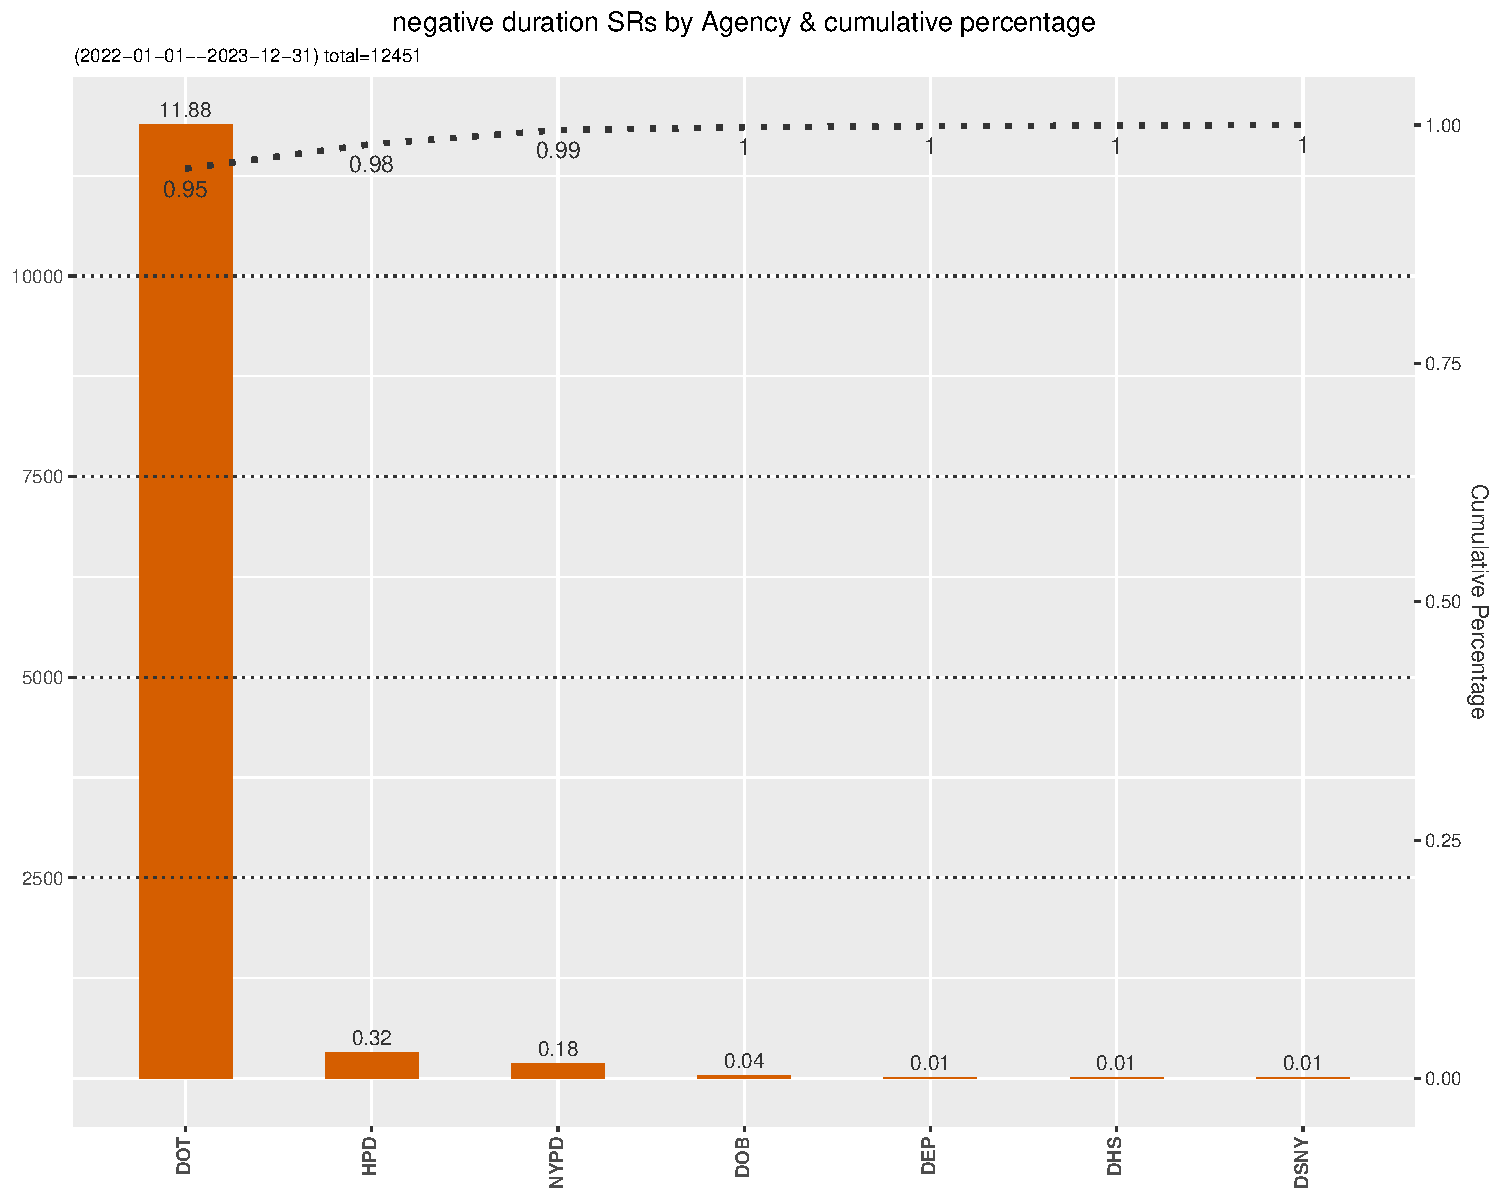
\includegraphics[width = \textwidth]{negative_duration_SR_barchart.pdf}
	  \label{fig:negative-duration}
\end{figure}

This violin chart shows the broad spread of negative-duration SRs, albeit with the extremely large 
negative-duration SR removed. While there are few outlier points, the magnitude of the negative-durations
is troubling and can produce bizarre analytical results.

\begin{figure}[tbp]
 	 \centering
 	 \caption{Distribution of Negative Durations}
	  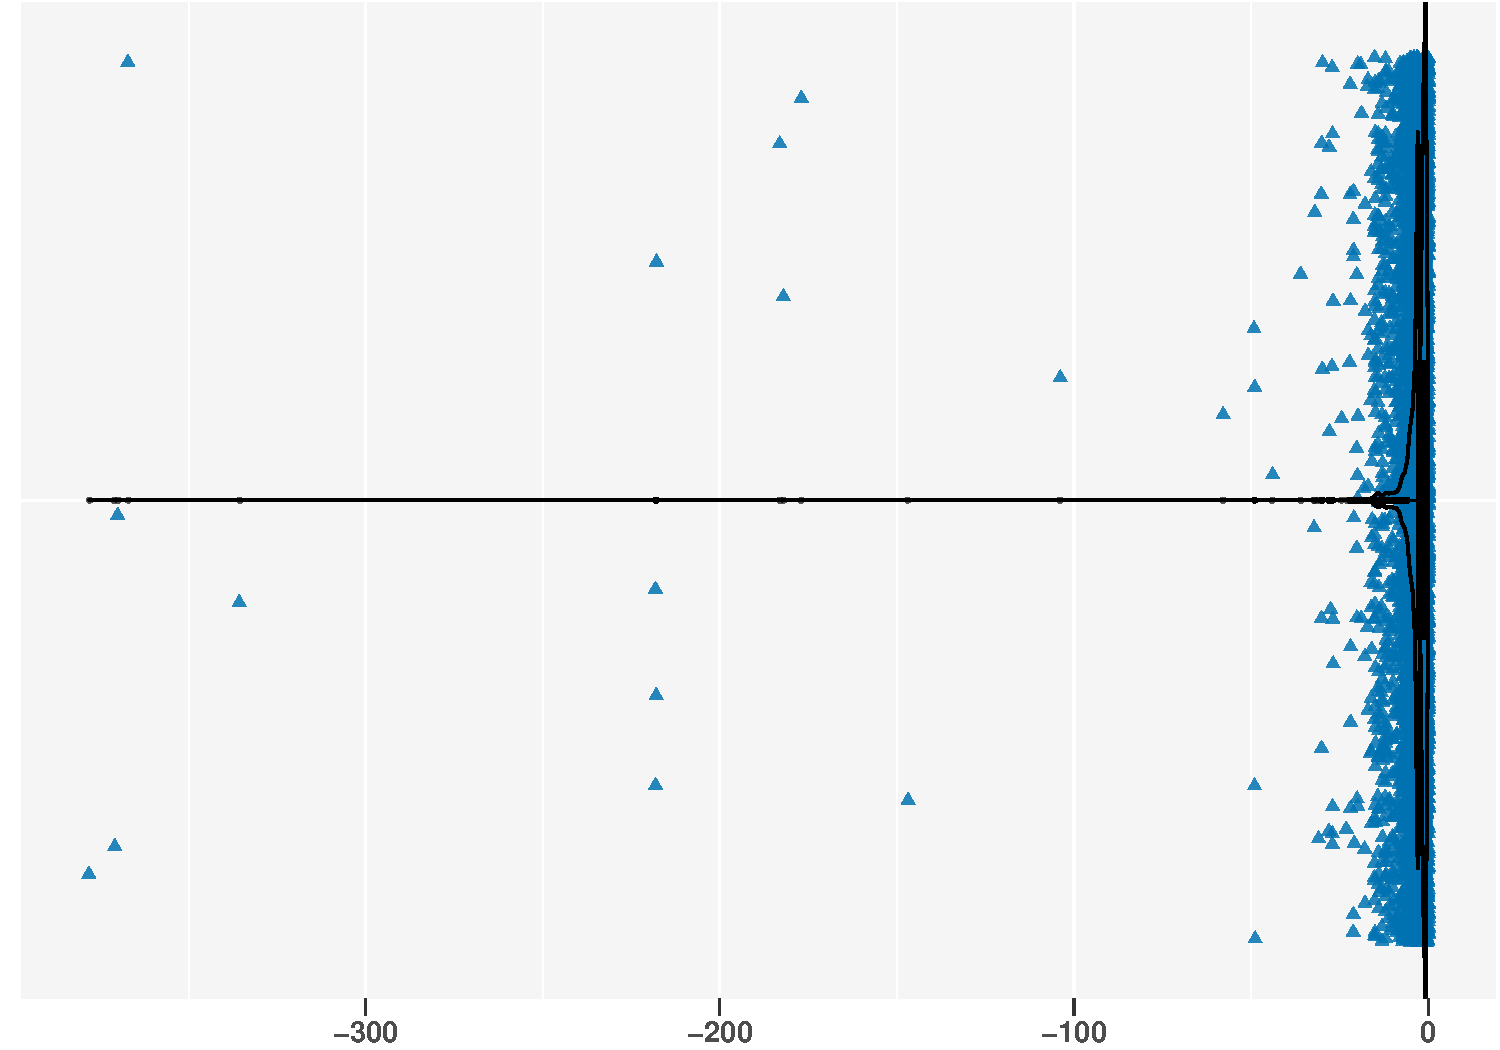
\includegraphics[width = \textwidth]{negative_duration_SR_violin.pdf}
	  \label{fig:negative-duration-violin}
\end{figure}


\subsubsection{Case Study: Homeless Person Assistance}
		\textbf{Scenario:} The Dept. of Homeless Services wants to know ``How quickly are 311 calls for ``Homeless Person
		Assistance over the past two years?'' resolved. This is a typical request made by both the public and City government. It's a performance metric along the lines
		of ``How quickly is my Agency responding to ``critical'' requests, and does that performance vary by Borough, Zip Code, etc. 

		As an analyst, this appears to be a routine effort: 
		
		\begin{enumerate}
		    \item Select data from 2022-2023 and filter the data by complaint\_type = ``Homeless Person Assistance'' (yields 55,000 SRs)
		    \item Compute a new field ``duration'' (closed\_date – created\_date)
		    \item Take an average of the ``duration'' field == \textbf{Answer:  -4.8 days}  
		\end{enumerate}
		
		Clearly that answer is nonsensical. How did such a simple task result in an absurd answer? The answer lies in the computation of the
		``duration'' field. As it turns out, there are eight DHS SRs that have a closed\_date of ``1900-01-01''. Each of those SRs creates a 
		negative duration of -44,602 days (-122 years). So just those eight SRs with extreme negative duration values is enough to drive
		the average of the 75,000 Homeless Assistance SRs to a negative value, clearly incorrect.
		
		As it turns out the distribution of the ``Homeless Person Assistance'' is quite skewed due to a small number of long duration
		SRs. In this case, the median is a better measure of central tendency than the average. And the median of the duration
		field is  0.2 days (approx 5 hrs). Here is a look at the distribution of durations for the Homeless Person Assistance SRs showing
		the large outliers. 
		
		\begin{figure}[tbp]
		 	 \centering
		 	 \caption{Homeless Assistance SR Durations}
			  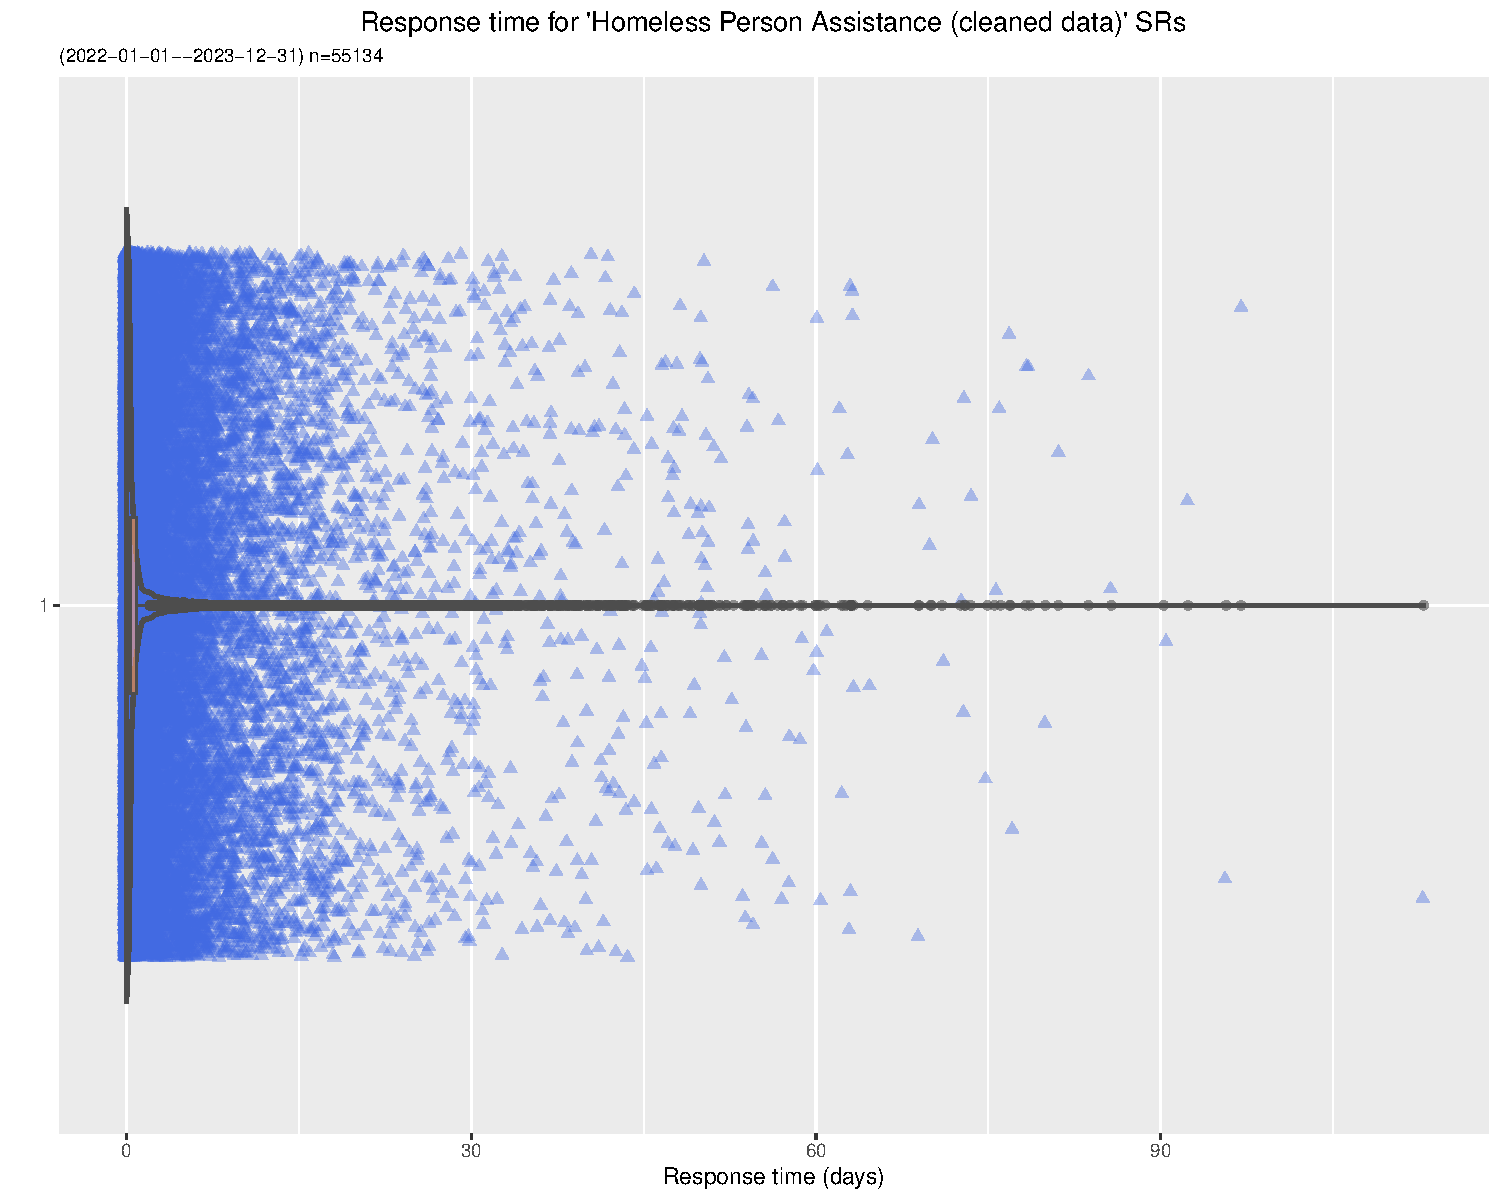
\includegraphics[width = \textwidth]{homeless_response_time_clean.pdf}
			  \label{fig:homeless}
		\end{figure}
		
	\subsection{created\_date and closed\_date(s) --  Zero Duration}		
	An even more serious, and more prevalent problem with closed\_date(s) occurs when the closed\_date and created\_date
	are exactly the same -- to the second -- which accordingly creates a \textbf{zero duration'}. Again this is nonsensical, but the
	presence of such zero durations can again severely distort analytics. There are 191,141 such SRs representing 3.1\% of all 
	non-blank data; not an insignificant number. As shown in the chart below, 99\% of the zero duration SRs appear to predominately
	occur in five Agencies (Dept of Mental Health \&Hygiene, Dept of Transportation, Dept of Business, Dept of Sanitation,
	and Dept of Environmental Protection.) This is not in-line with the overall Agency distribution of SRs and indicates an
	Agency-specific issue, and the solution likely lies at those Agencies.
	
	\begin{figure}[tbp]
		 \centering
		  \caption{SRs with Zero Durations by Agency}
		 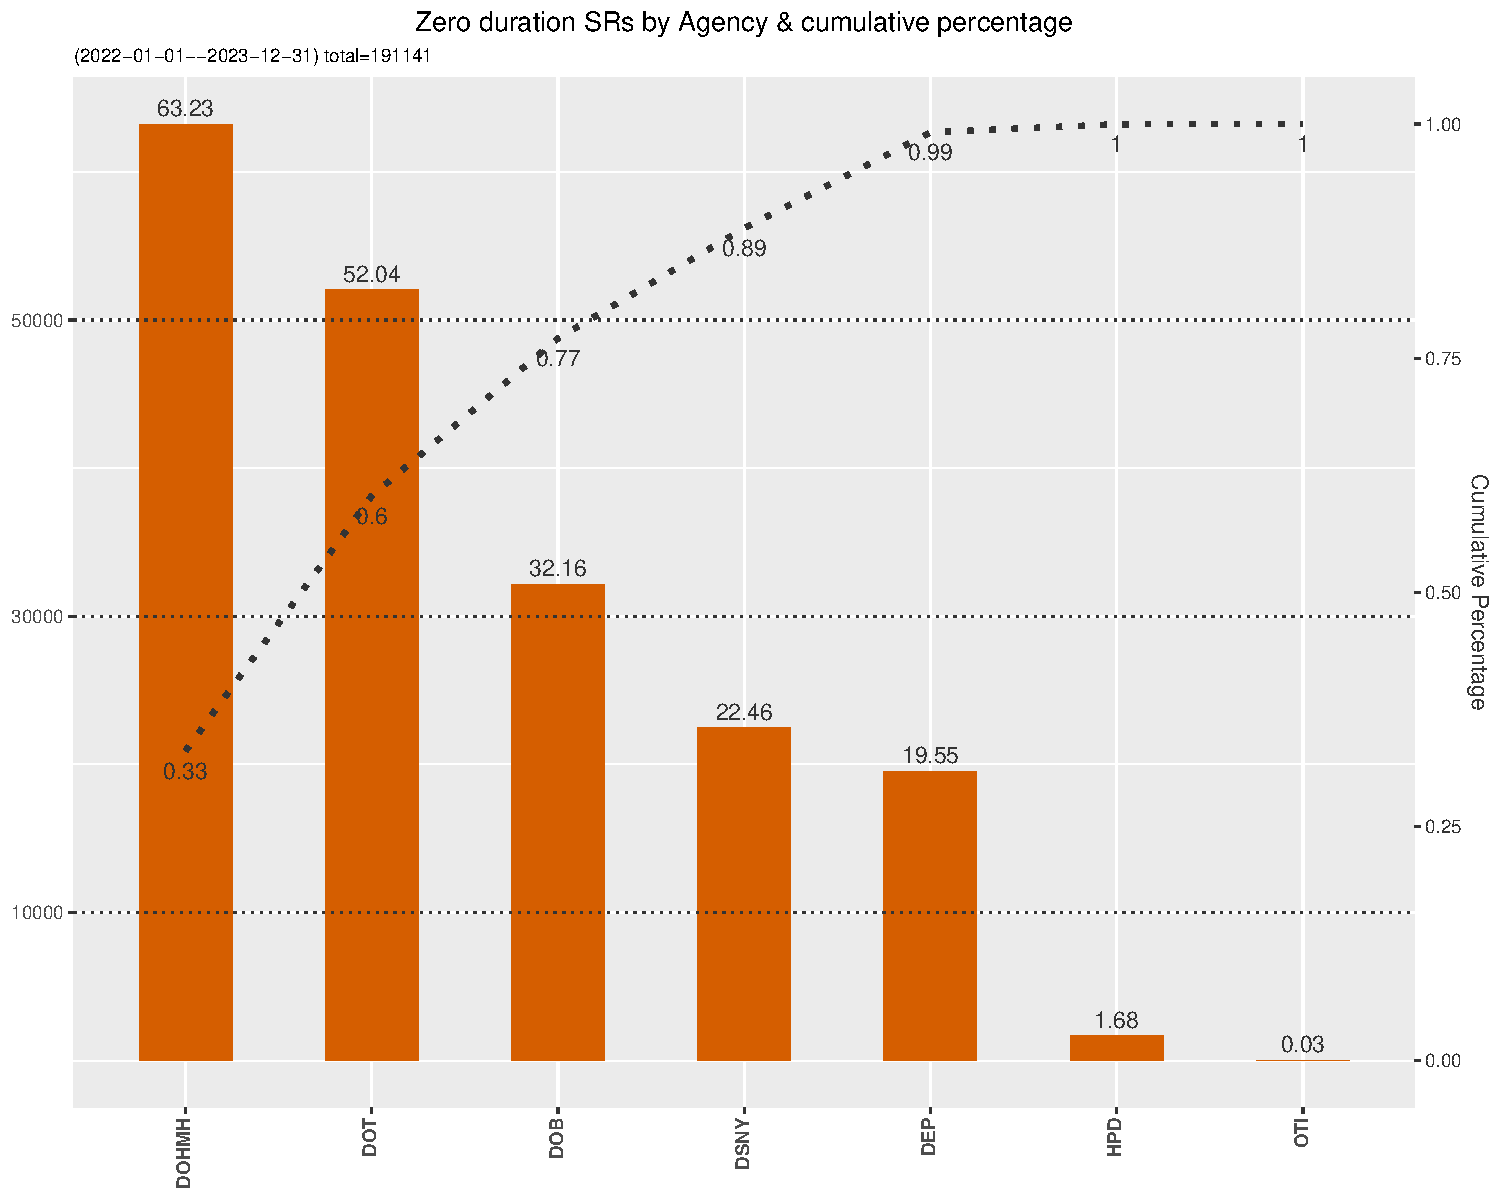
\includegraphics[width = \textwidth]{zero_duration_SR.pdf}
		 \label{fig:zero-duration}
	\end{figure}	
		
	\subsection{created\_date and closed\_date(s) -- Midnight \&Noon}
	An additional problem discovered with the created\_date and closed\_date fields; there appears to be an unusually large number of 
	SRs created or closed at exactly midnight (00:00:00) and exactly noon (12:00:00), to the second. The distribution of SR creation and closure 
	largely follows the work-day clock with many SRs created during day-light hours, and fewer SRs 
	created at night and in the early hours of the morning. 
	However, here there appears to be significantly greater numbers of SR closed exactly at midnight and exactly at noon,
	as well as a significant number of SRs created exactly at noon. The reason behind this anomaly is worth investigating 
	as it affects the SR ``duration'' question. If SR durations are used to measure responsiveness
	for the delivery of services, and if those times are not an accurate reflection of the start/finish of the Service, then the use of
	duration as a service quality metric is called into question. Observations during this 2-year period include:
	
	\begin{itemize}
		    \item There were 99,779 SRs created exactly at noon (12:00:00)
		    \item There were 235,347 SRs closed exactly at midnight (00:00:00)
		    \item There were 105,505 SRs closed exactly at noon. 
	\end{itemize}
	
	There is, of course, a broad distribution of the time that SRs are created by day and hour, by night and day, by weekday and weekend. 
	One would think that that distribution would be (mostly) evenly distributed by the minute and second. That is, 
	if there are normally 100 SRs created between 1-2pm, that the distribution to the minute and second 
	would be close to random. For example, there is no reason to suspect that a larger number of SRs would be 
	created at 6 minutes past the hour rather than at 5 minutes past the hour. And certainly, if you look at the second that these SRs
	are created you would again expect a (more-or-less) random distribution; that there would be no reason to believe 
	that a higher (or lower) number of SRs would arrive at 18 seconds past the minute versus at 39 seconds past the minute.
	Unfortunately, that turned out not to be true.
	
	Let's look at the SR creation distribution. We discovered that there are a significant number of SRs created exactly at noon. To reveal this
	trend, we looked at the exact date-time stamp of the created\_date(s). We began by selected only SRs that were created exactly on the minute;
	at 09:00:00 or 13:00:00 for example.  Here is a visualization of the number of SRs created and closed by hour-of-the-day:
	
	\begin{figure}[tbp]
		\centering
		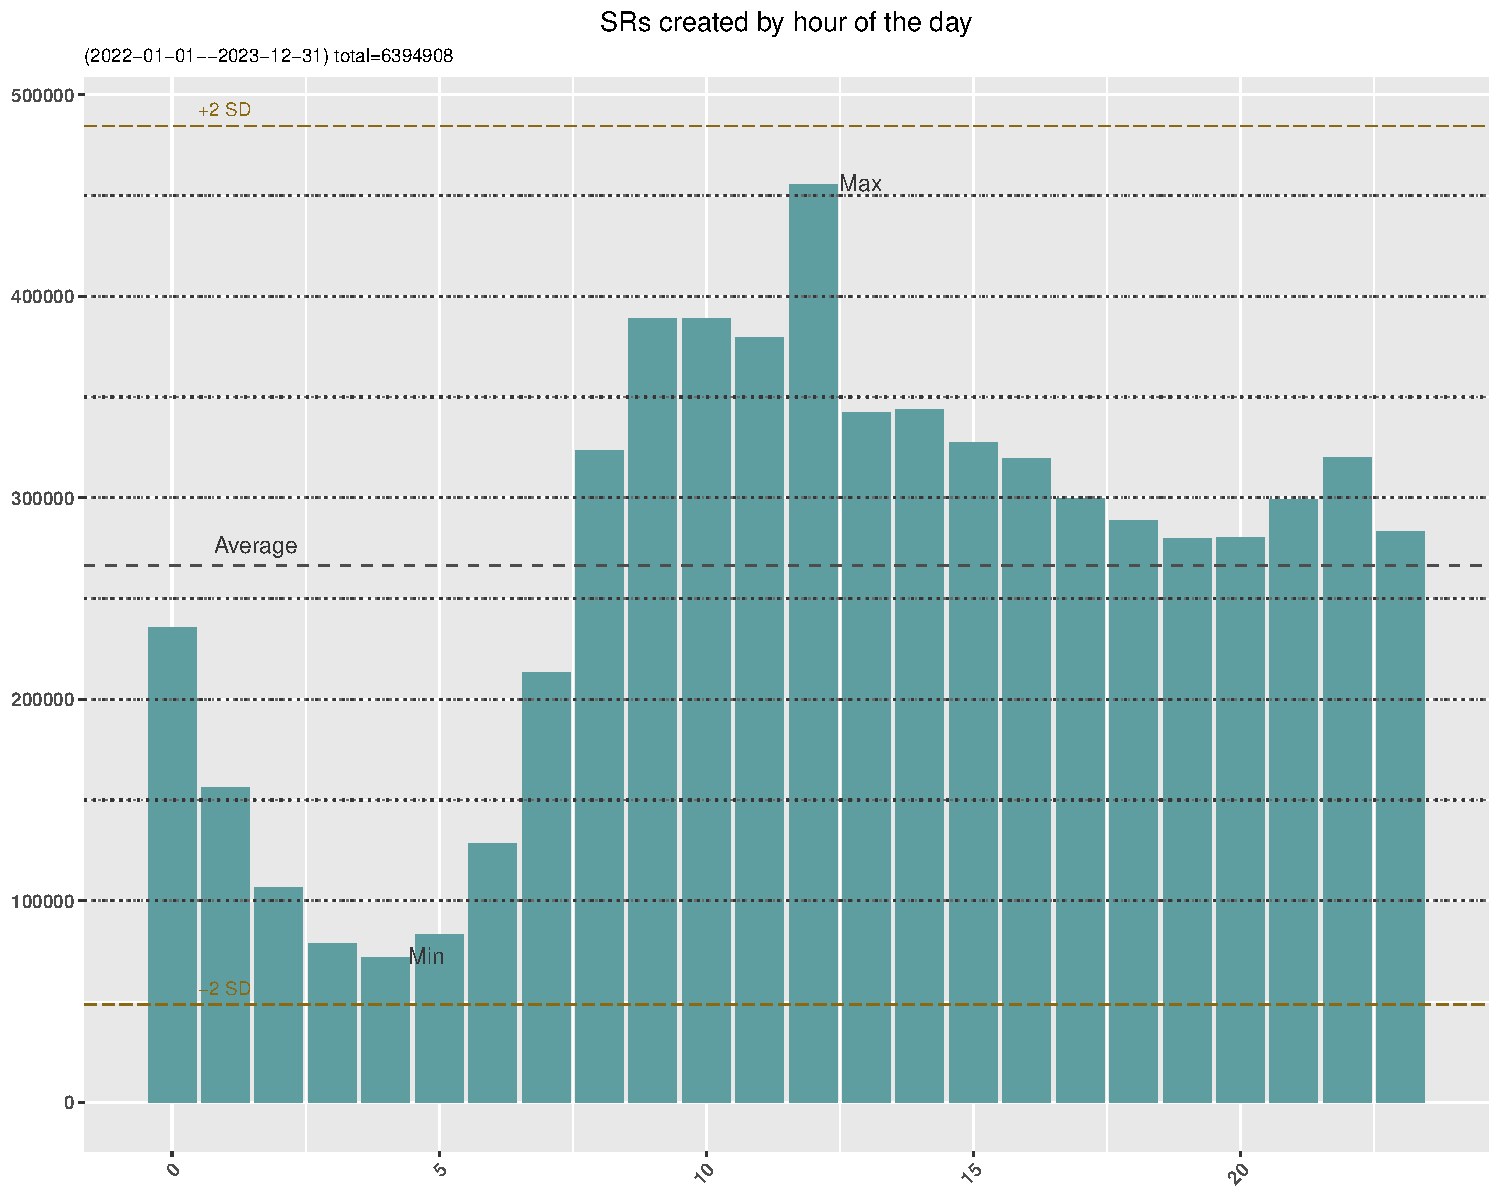
\includegraphics[width = \textwidth]{Created_Hourly_SR_count.pdf}
		\caption{SRs by Hourly created\_date(s)}
		\label{fig:hourly-created}
	\end{figure}	
	
	\begin{figure}[tbp]
		\centering
		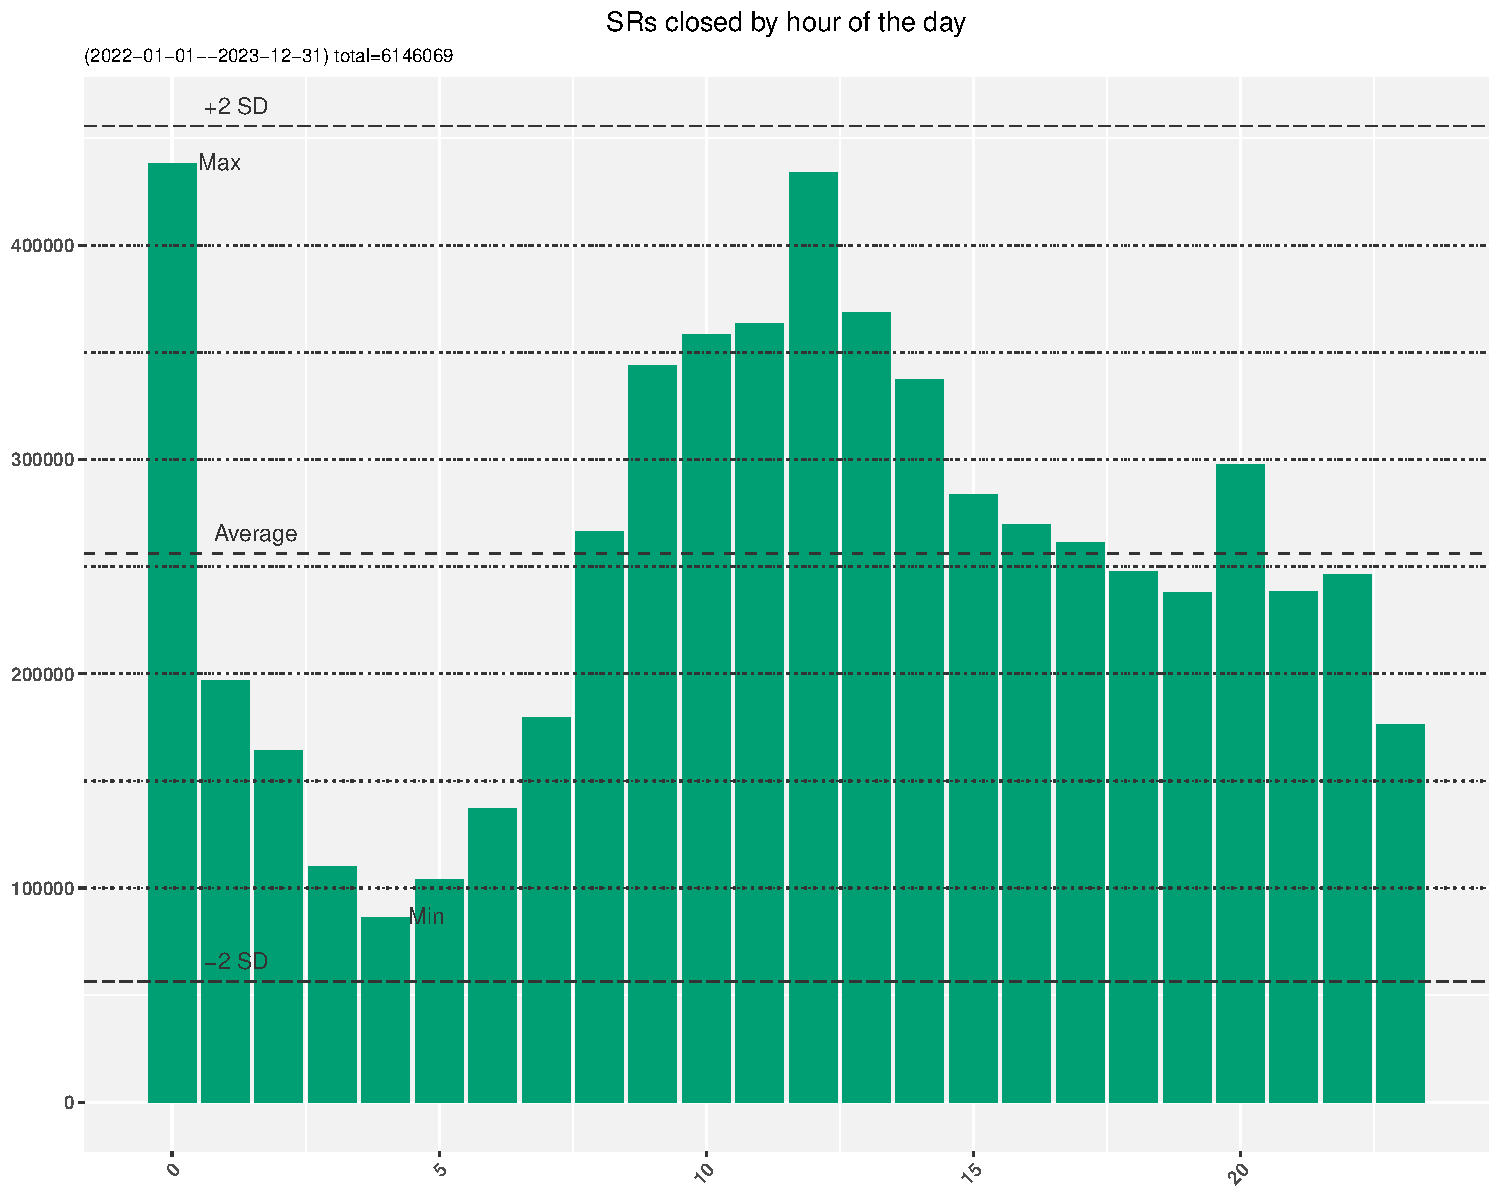
\includegraphics[width = \textwidth]{Closed_Hourly_SR_count.pdf}
		\caption{SRs by Hourly closed\_date(s)}
		\label{fig:hourly-closed}
	\end{figure}	
	
	The created\_date shows a maximum value at 12:00. The closed\_date chart show significant spikes at both midnight
	and noon. The midnight (00:00) spike appears to be an anomaly especially as compared to the hours just 
	before and after midnight where there is normally a pronounced slump in SR closures. 
	And both the closed-at-noon and closed-at-midnight are approaching 2\textsigma's from the hourly average. 

	Let's drill down on each of these outlier points. First, we aggregate the created\_date over the 2-year period that fall exactly
	on the top-of-the-hour with the minute and second values equal to 0, e.g. 09:00:00, 14:00:00. This visualization
	reveals a clearer picture of where these spikes are:
	
	\begin{figure}[tbp]
		\centering
 		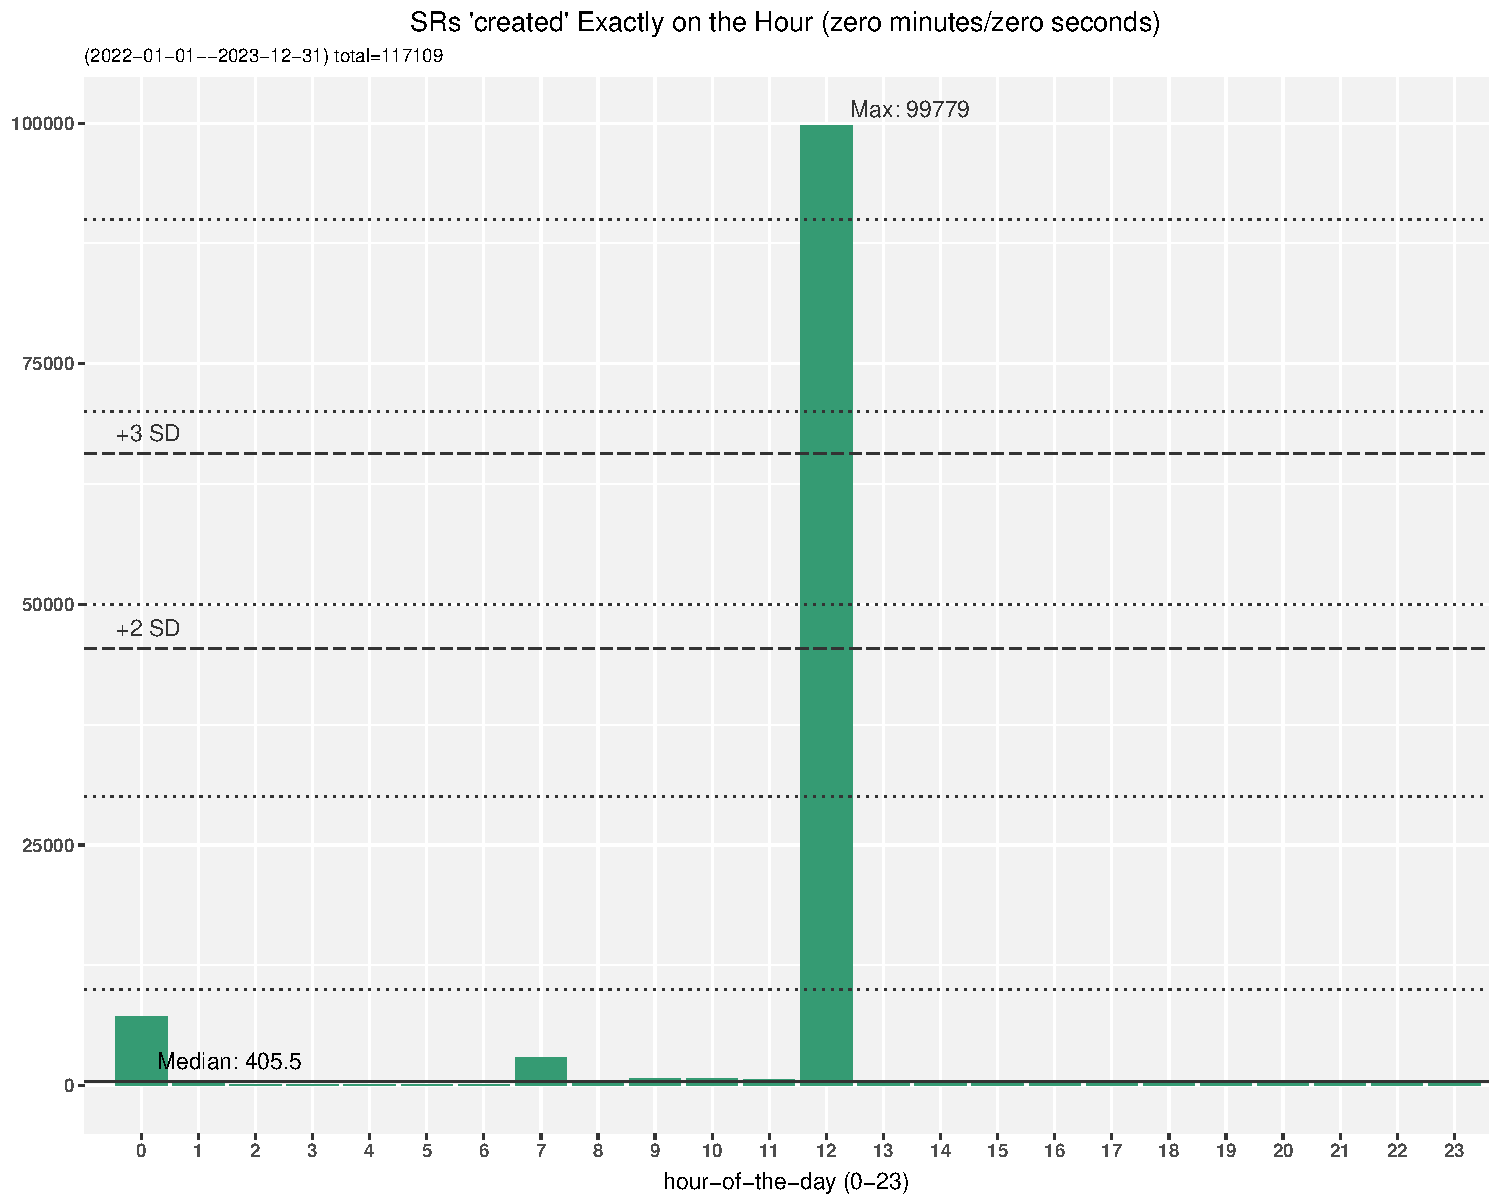
\includegraphics[width = \textwidth]{2-year-trend-SR_created_by_top_of_hour.pdf}
		\caption{SRs Created at Top-of-the-Hour}
		\label{fig:tophourcreated}
	\end{figure}	

	One other way to visualize this anomaly is to look at the busiest day during this 2-year period (Friday, 2023-09-29).
	Here we will aggregated the created\_date(s) by minute (with seconds equal to zero). This provides a 
	minute-by-minute look at SR creation on the busiest day of this study. Here we see a clear spike at 
	exactly noon (12:00), well beyond the 3\textsigma line, and well above any other hour of the day.
	
	\begin{figure}[tbp]
		\centering
		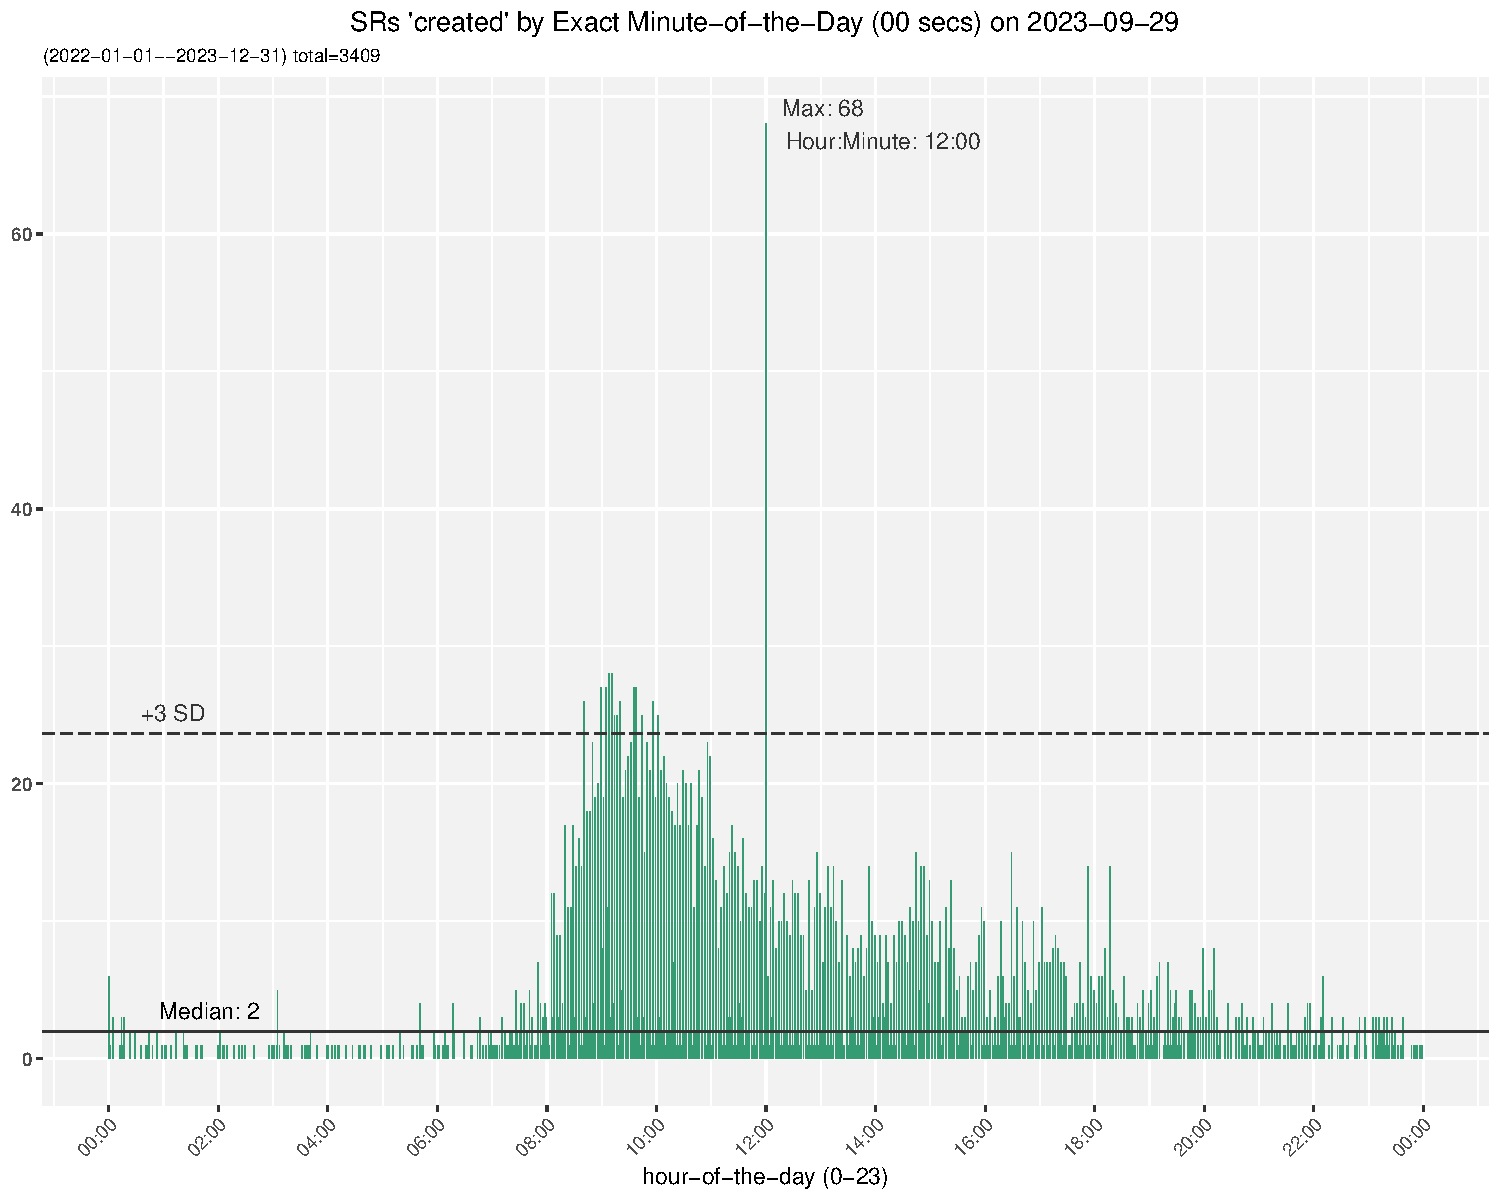
\includegraphics[width=\textwidth]{2-year-trend-SR_created_by_minute_of_busiest_day.pdf}
		\caption{SRs Created Minute-by-Minute on Busiest Day}
		\label{fig:busiestcreated}
	\end{figure}	

	Let's take a similar approach to the closed\_date distribution over the 2-year period. We aggregate 
	SRs by close\_date to find the top-of-the-hour, where minute and second values equal to 0, e.g. 20:00:00. 
	Here we see spikes at both midnight (00:00) and at noon (12:00), with the midnight spike being 
	well beyond the 3\textsigma line. Also note how much lower (and nearly equal) all the other
	top-of-the-hour values are, relative to the midnight and noon spikes. 
	
	\begin{figure}[tbp]
		\centering
		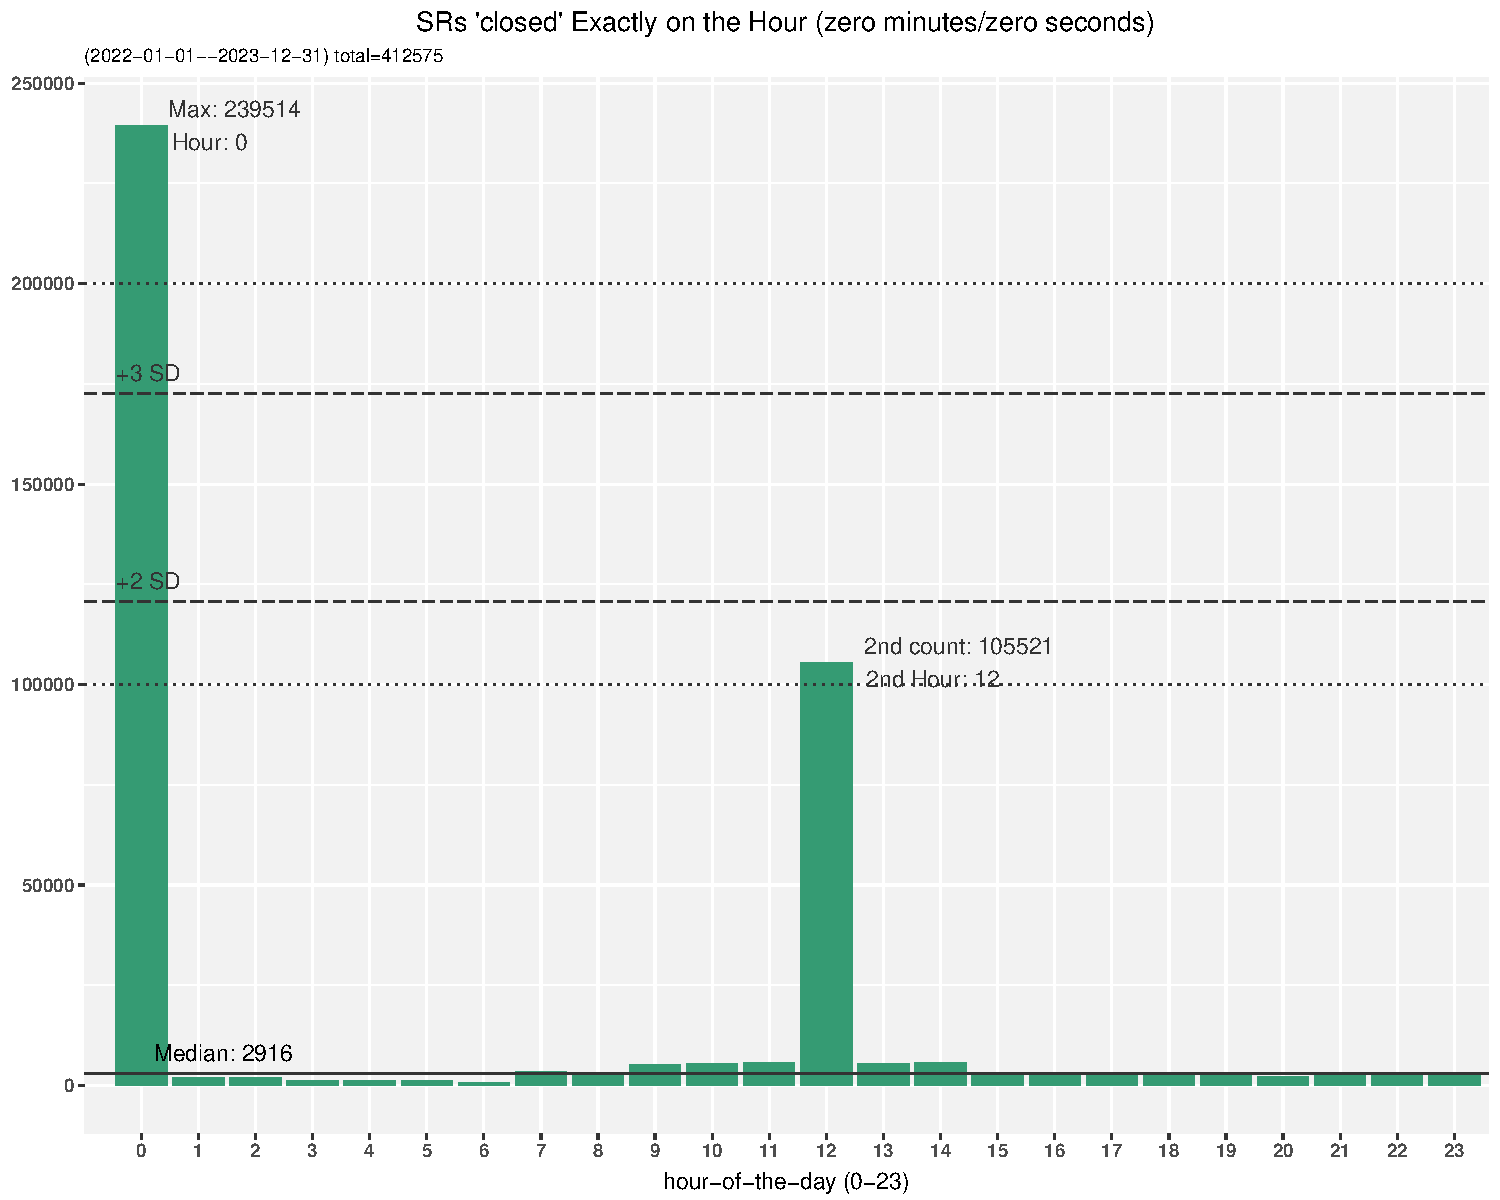
\includegraphics[width = \textwidth]{2-year-trend-SR_closed_by_top_of_hour.pdf}
		\caption{SRs Closed at Top-of-the-Hour}
		\label{fig:tophourclosed}
	\end{figure}
	
	As before, let's visualize this anomaly by looking at the closed\_date(s) on the busiest day
	during this 2-year study period (Friday, 2023-09-29). We aggregate closed\_date(s) by the
	minute (with seconds equal to zero). This gives a minute-by-minute view of SR closure
	on the busiest day of this study. Clearly visual is the very large closure spikes occurring
	at both midnight and noon. The chart highlights both of these anomalies with spikes
	of 286 and 120 at 00:00:00 and 12:00:00 respectively. Again, note how these spikes
	are so very much above the median values for all other minutes.

 	\begin{figure}[tbp]
		\centering
		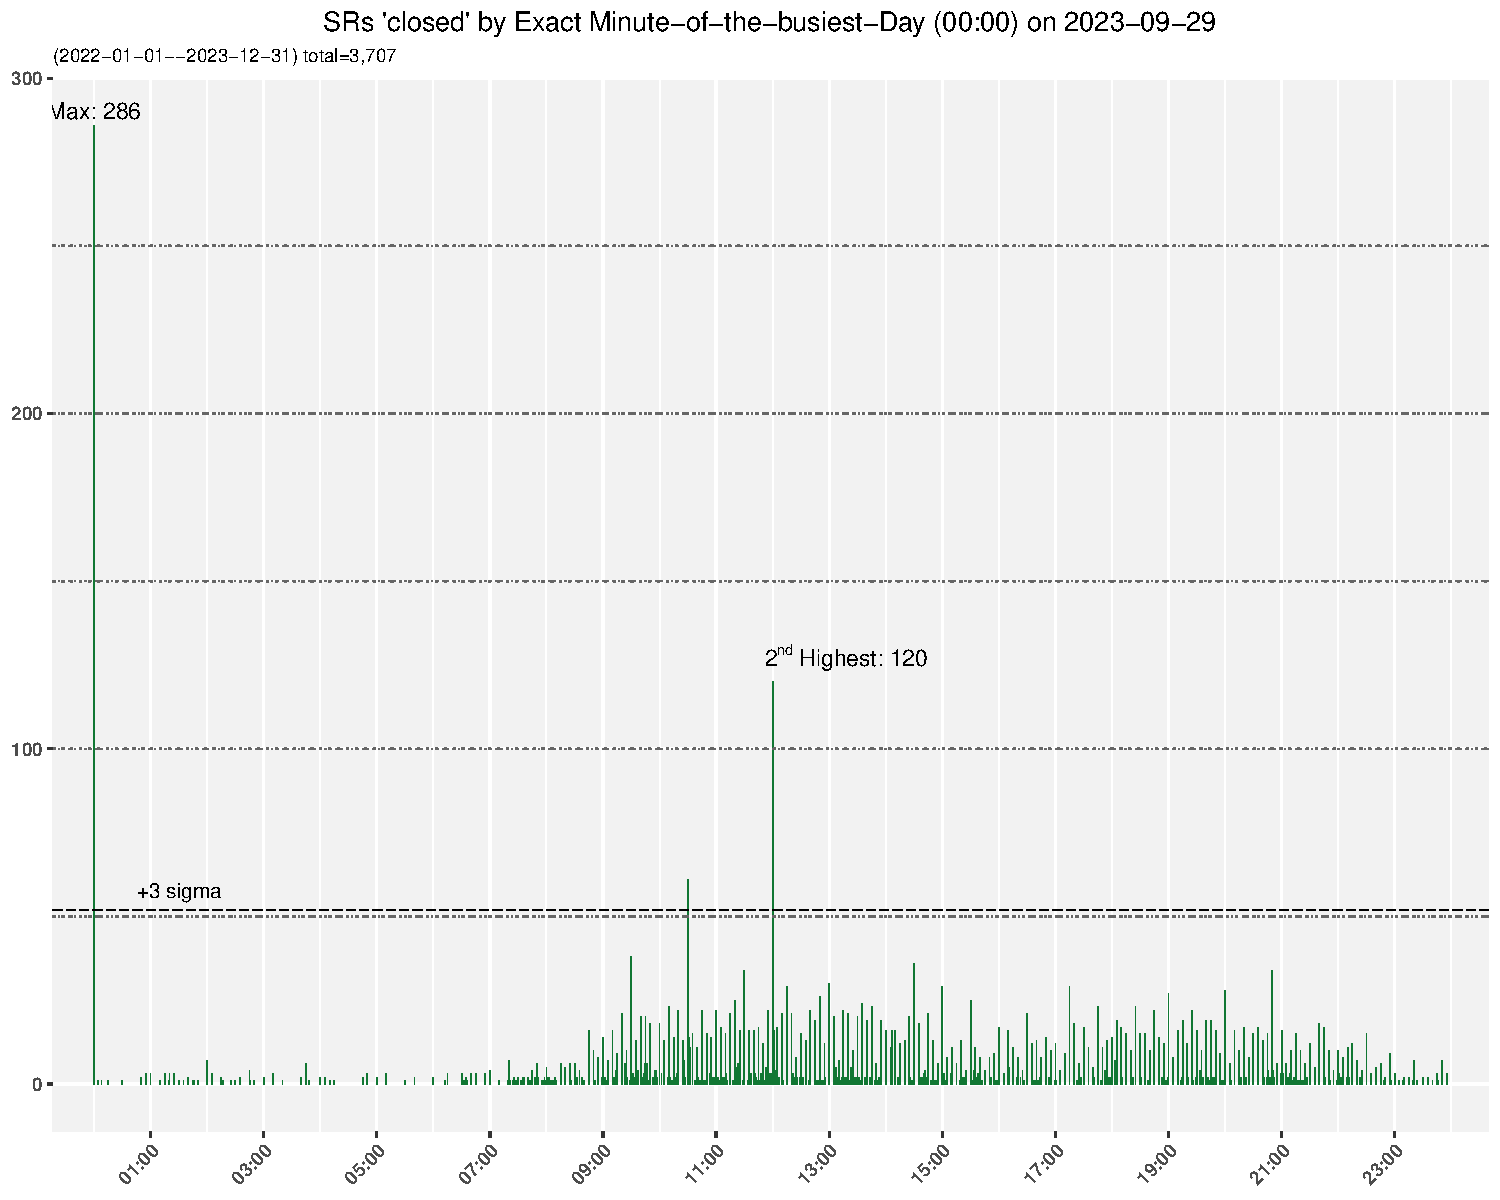
\includegraphics[width=\textwidth]{2-year-trend-SR_closed_by_minute_of_busiest_day.pdf}
		\caption{SRs Closed Minute-by-Minute on Busiest Day}
		\label{fig:busiestclosed}
	\end{figure}	

	These unusual patterns of created \& closed SRs at exactly the hours of midnight and noon likely indicates
	the presence of a bulk create/close software process; a process that perhaps automatically ``closes'' (or ``creates'') 
	a large number of SRs with a provided time-stamp of midnight (00:00:00) or noon (12:00:00), and does so in bulk. 
	If so, then addressing this issue likely requires a closer look at those Agencies providing these suspect SR closed/created times.
	 The desirable state is that the created\_date and closed\_date fields correctly reflect the true opening and closing 
	 of the SRs, such that an accurate ``duration'' can be computed for the SR life-cycle. Otherwise, we are likely seeing 
	 durations that are artificially manipulated by a software process performing bulk uploads to the 311 system.

	Looking at the distribution by Agency for the ``closed-exactly-at-midnight'' shows that \textgreater90\% of these suspect SRs come from just two Agencies - Dept. of 
	Buildings (DOB) and Dept. of Sanitation (DSNY). If you include HPD and DOT, that accounts for 99\% of the suspect SR closures. This Agency
	distribution does not follow the overall SR distribution and we can assume that it is Agency specific. 

	\begin{figure}[tbp]
		\centering
		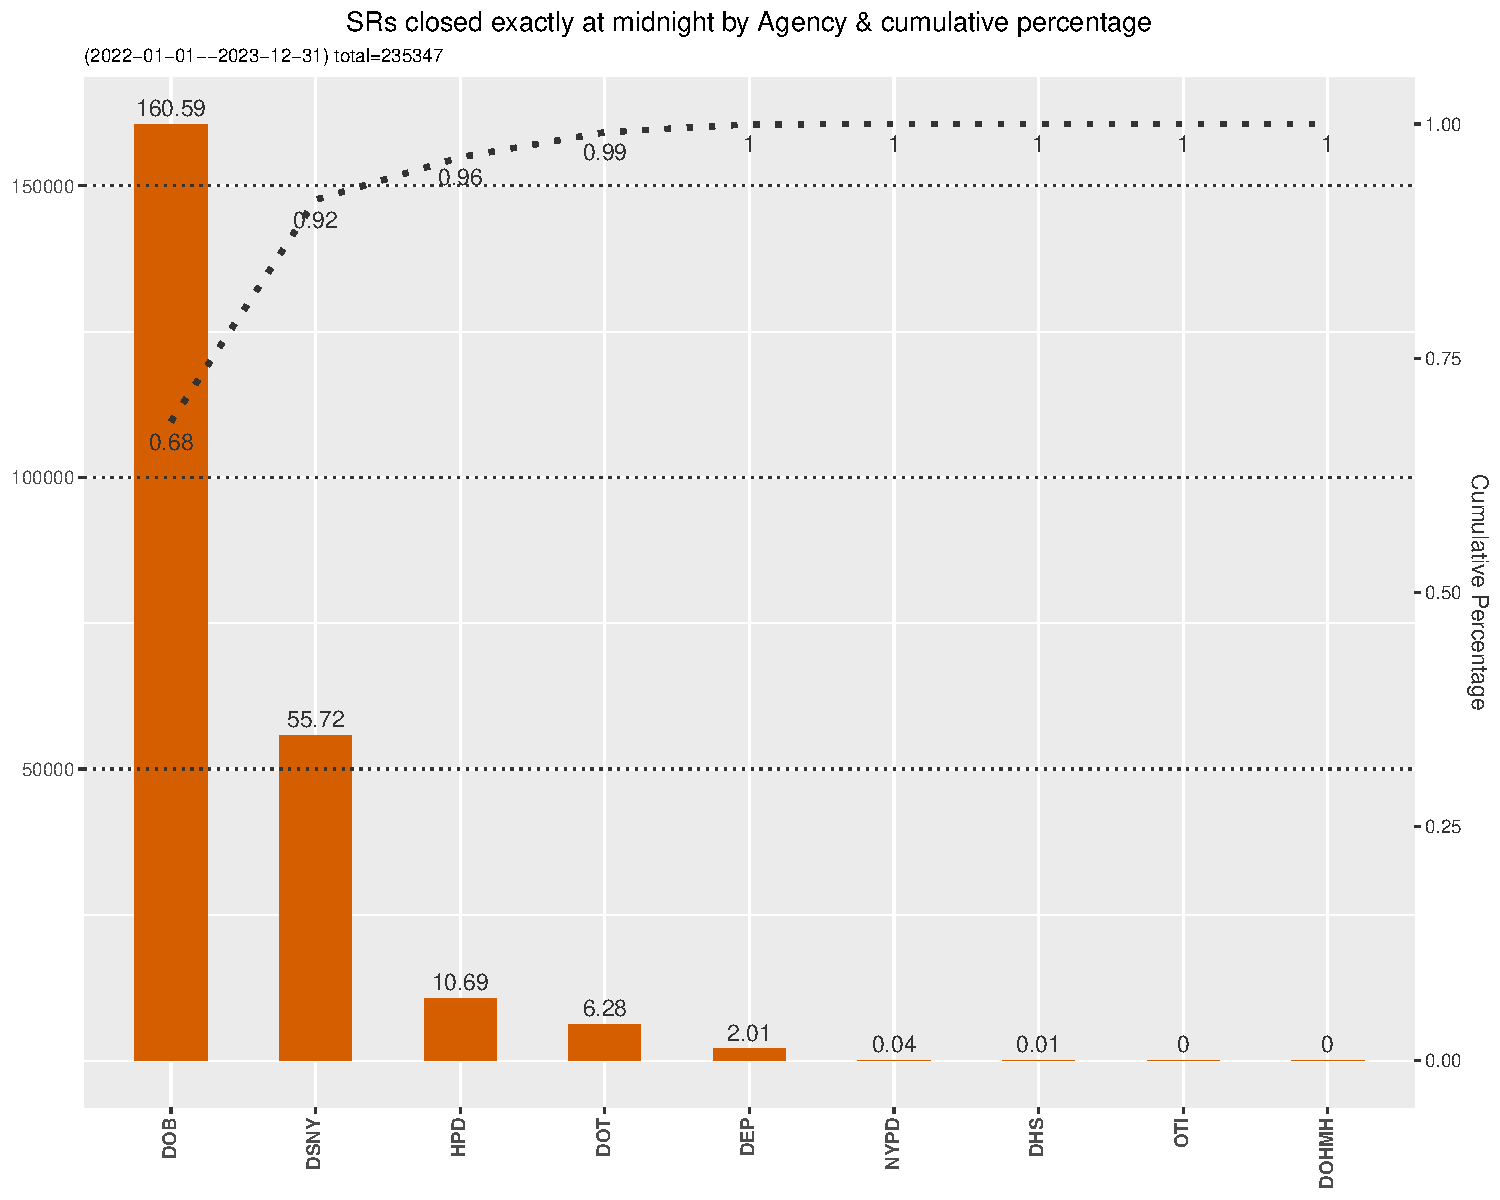
\includegraphics[width = \textwidth]{closed_at_midnight_chart.pdf}
		\caption{SRs Closed Exactly at Midnight by Agency}
		\label{fig:midnight-closed}
	\end{figure}	

	However, the ``SR closed at noon'' visualization shows that  a single Agency, DSNY,
	is responsible for \textgreater99\% of the SRs ``closed-exactly-at-noon''. Accordingly, any effort to resolve this issue
	necessitates working with DSNY to fully understand how this is occurring. 
	
	\begin{figure}[tbp]
		\centering
		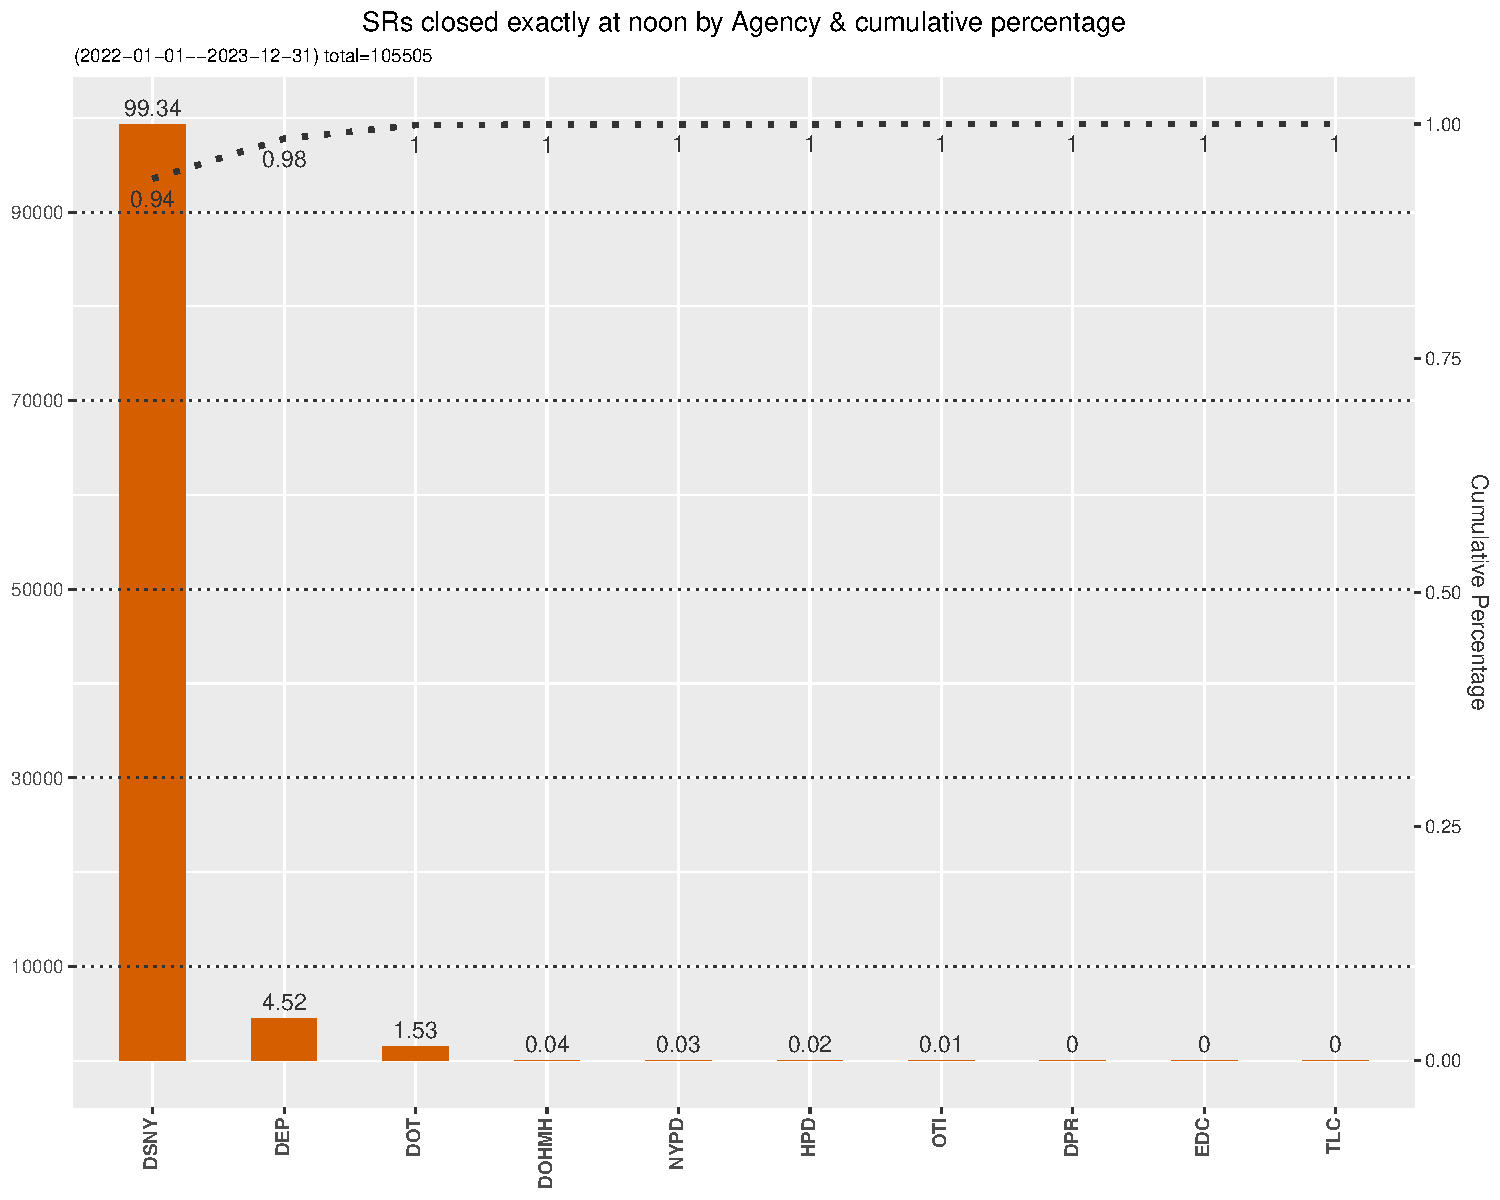
\includegraphics[width = \textwidth]{closed_at_noon_chart.pdf}
		\caption{SRs Closed Exactly at Noon by Agency}
		\label{fig:noon-closed}
	\end{figure}	
	
	The 99,779 SRs created-exactly-at-noon also appears to originate with the Dept of Sanitation (DSNY) which
	is responsible for \textgreater99\% of the suspect SRs.
	
	\begin{figure}[tbp]
		\centering
		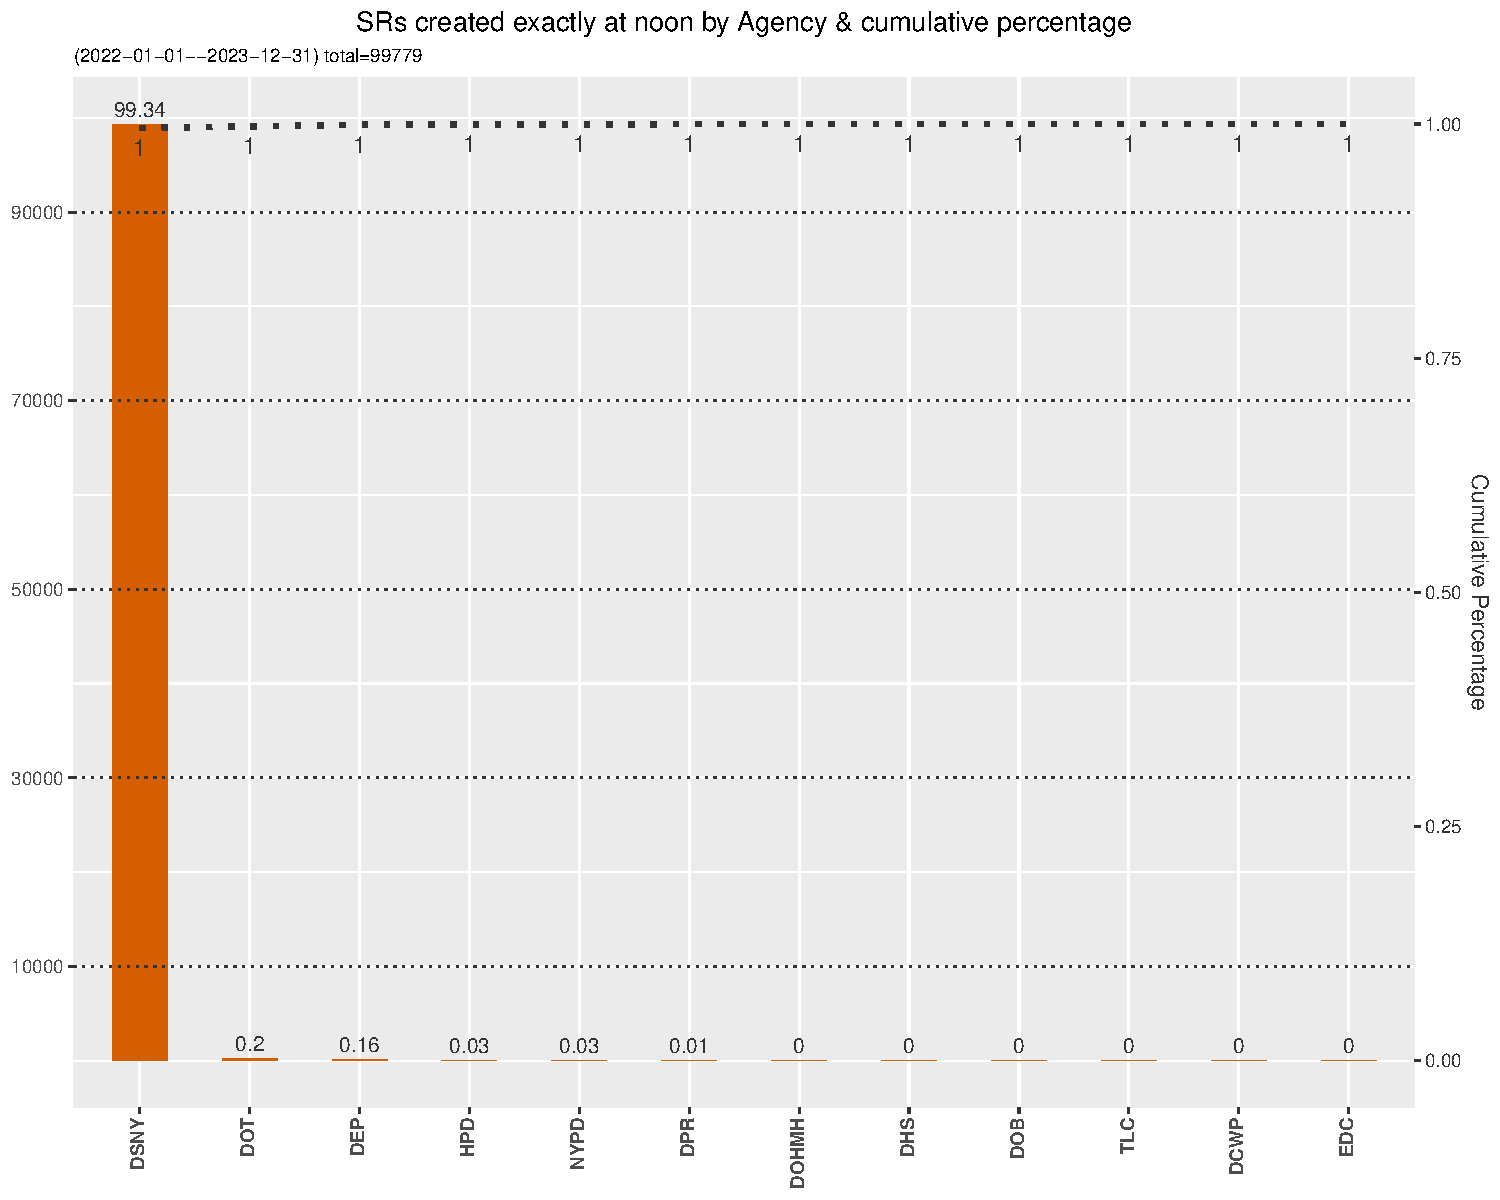
\includegraphics[width = \textwidth]{created_at_noon_chart.pdf}
		\caption{SRs Created Exactly at Noon by Agency}
		\label{fig:noon-created}
	\end{figure}		
		
	While it is difficult to ultimately know if these observations are indeed anomalies; they could be the result of normal, expected
	311 SR activity. But at least by observation that outcome appears very unlikely.	
		
	\subsection{resolution\_action\_update\_date}
	When an SR is updated, by any means on any field, the software automatically populates the resolution\_action\_update\_date. Analyzing that field
	it is apparent that some of the SR updates are happening long, long after the SR is closed. In this dataset there are eight SRs that have 
	resolution\_action\_update\_date values of 44,601 days after the closed\_date. The problem lies not with the resolution\_action\_update\_date, but
	rather with the closed\_date values for these 8 SRs, all of which are in the format of ``1900-01-01''. It has previously been discussed that these
	inaccurate dates may possibly be coming from an Excel spreadsheet as that is the minimum date which Excel can handle. Here is a sample
	of those SRs:

	\begin{table}[tbp]
	    \centering
	    \caption{Extremely long Resolution Updates}
	    \normalsize
	    \begin{tabular}{cccc}
	        \hline
	        Agency & Closed Date & Resolution Action Updated Date & Post Closed Update Duration (days) \\
	        \hline
	        DHS & 1900-01-01 & 2022-02-12 00:58:43 & 44602 \\
	        DHS & 1900-01-01 & 2022-02-11 14:28:59 & 44601 \\
	        DHS & 1900-01-01 & 2022-02-11 14:17:41 & 44601 \\
	        DHS & 1900-01-01 & 2022-02-11 13:45:59 & 44601 \\
	        DHS & 1900-01-01 & 2022-02-11 13:22:12 & 44601 \\
	        \hline
	    \end{tabular}
	    \label{tab:resolution-updates}
	\end{table}
	
	These obvious inaccurate date values are removed from the analysis. But even so, there are some very late
	updates to SRs, with some updates occurring almost two years after the SR is closed.   There are a total of 7460 SRs that are 
	updated \textgreater30 days and \textless{}730 days after the closed\_date. The median of these late (\textless{}30 days)
	post-closed resolution\_action\_update\_date(s) is 84 days. However, the mean resolution\_action\_update\_date 
	for all of the SRs is only 0.39 days (9.3 hours) after the SR is closed. It is not known if this is normal behavior
	or an area that may require further investigation. 
	
	\begin{table}[tbp]
    \centering
     \caption{Long post-closed Resolution Updates}
    \normalsize
	    \begin{tabular}{cccc}
	        \hline
	        Agency & Closed Date & Resolution Action Updated Date & Post Closed Update Duration (days) \\
	        \hline
	        TLC & 2023-05-25 14:21:12 & 2023-10-19 10:57:02 & 147 \\
	        TLC & 2023-07-12 11:03:46 & 2023-12-07 09:00:05 & 148 \\
	        TLC & 2023-08-03 10:34:23 & 2024-01-29 10:00:37 & 179 \\
	        TLC & 2022-04-04 10:54:39 & 2022-06-02 12:14:11 & 59 \\
	        TLC & 2022-12-05 15:23:45 & 2023-02-02 09:06:45 & 59 \\
	        \hline
	    \end{tabular}
    \label{tab:resolution}
	\end{table}

	Here is a look at the spread of the post-closed resolution\_action\_update\_date values those SRs 
	that are \textgreater30 days and \textless{}730 days. There are some significant outliers 
	
	\begin{figure}[tbp]
		\centering
		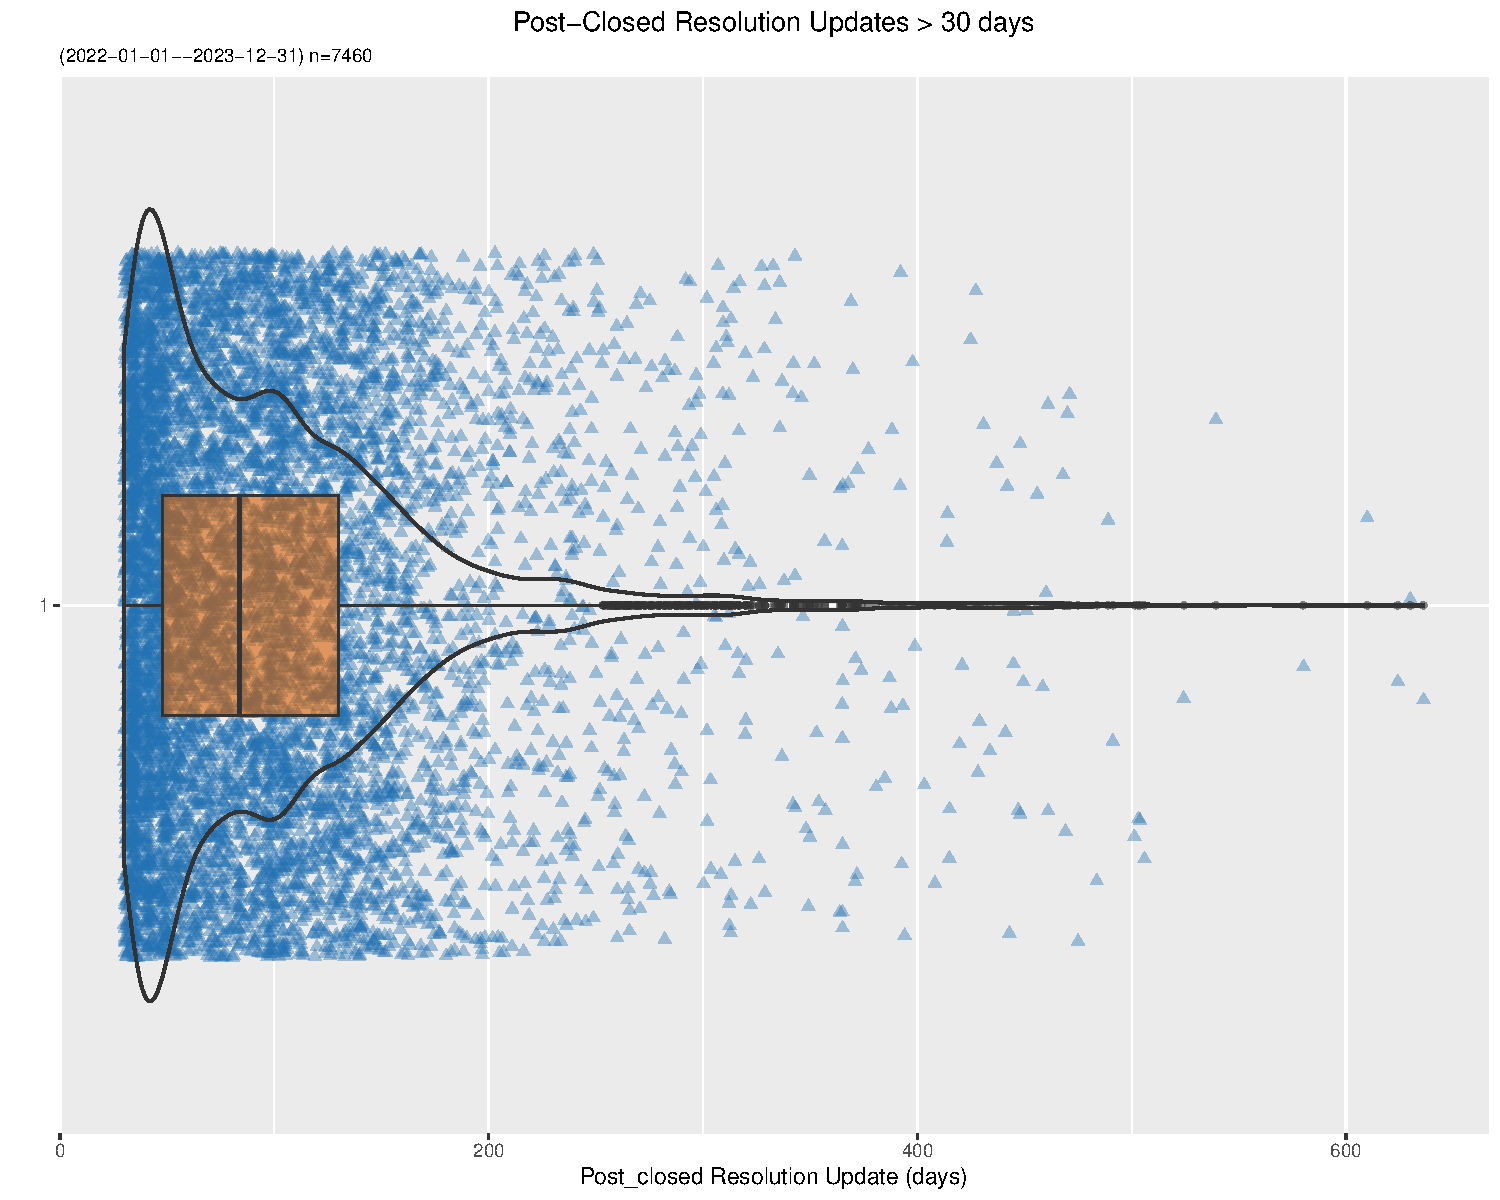
\includegraphics[width = \textwidth]{post_closed_violin.pdf}
		\caption{Post-Closed resolution\_action\_update\_date(s) \textgreater30 days}
		\label{fig:resolution-violin}
	\end{figure}		

	If we look at a breakout of these (late?) update dates by Agency, we can see that the vast majority li with two
	Agencies: Taxi \& Limo Commission (TLC) and Dept of Sanitation (DSNY) which account for 96\% of the SRs in
	question.  Is there a valid reason that TLC and DSNY would be updating an SR over month (or months) after
	the SR has been closed? Perhaps, but it seems to merit closer investigation. 

	\begin{figure}[tbp]
		\centering
		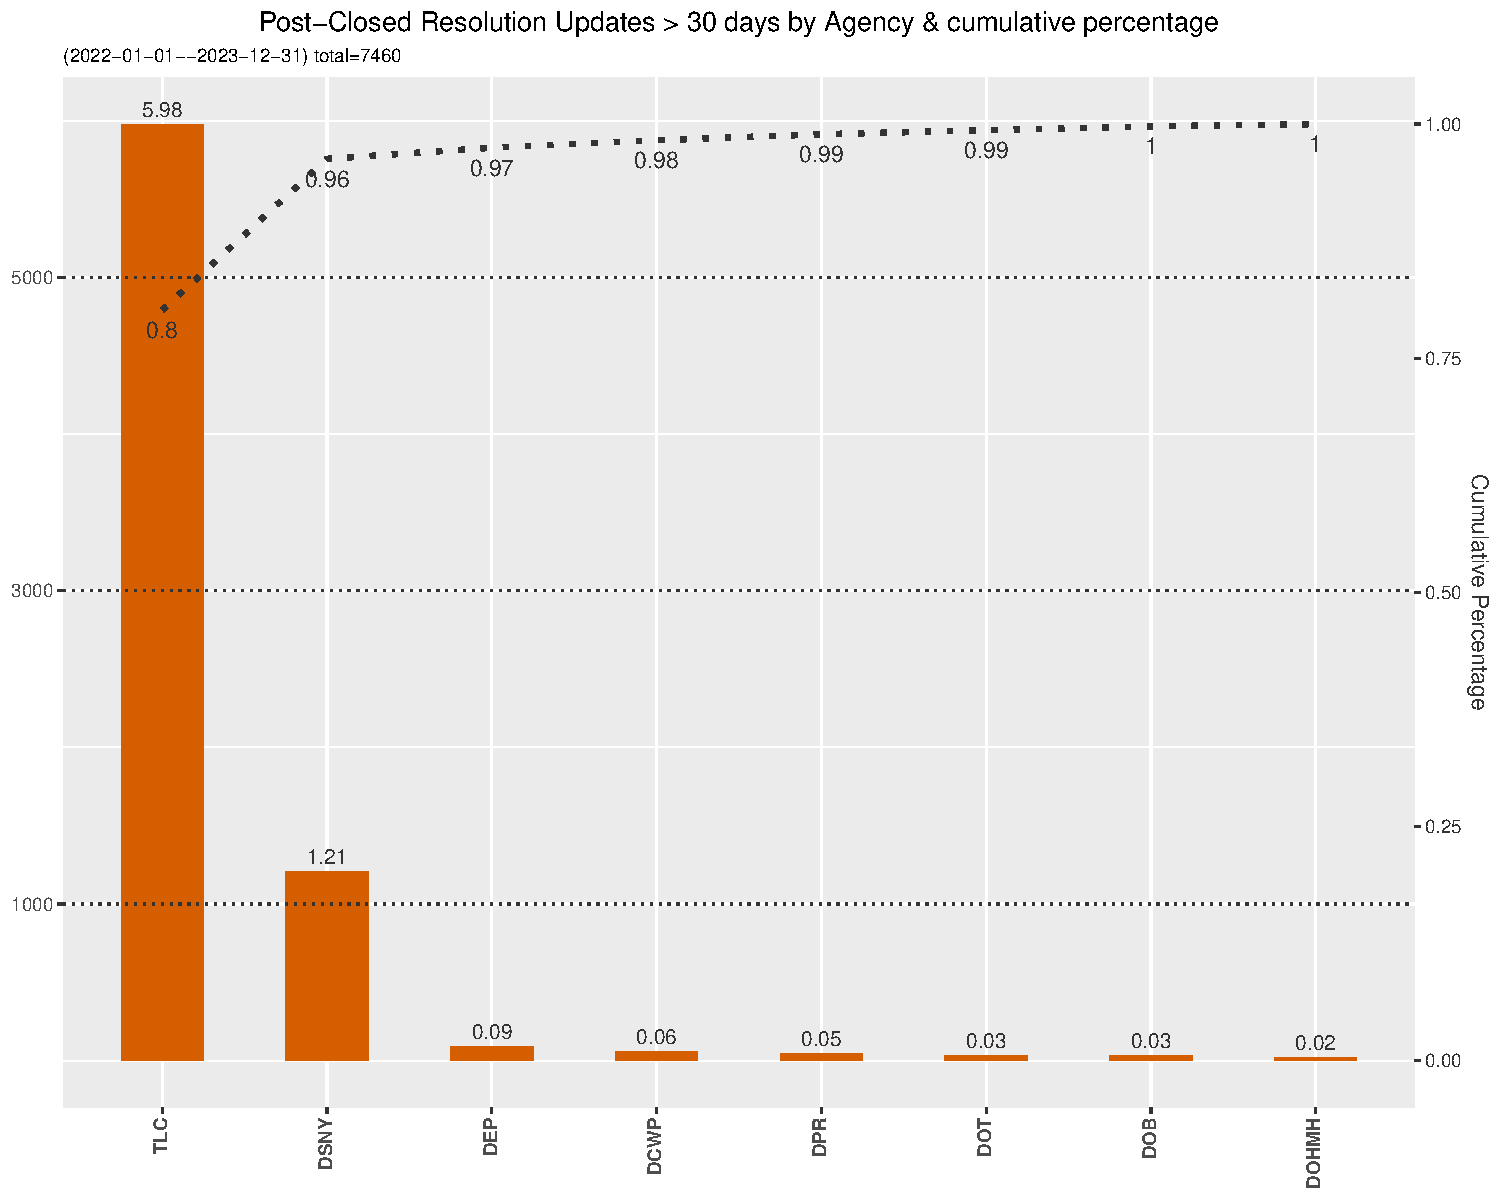
\includegraphics[width = \textwidth]{postClosedBarChart.pdf}
		\caption{Post-Closed resolution\_action\_update\_date(s) \textgreater30 days by Agency}
		\label{fig:resolution-by-agency}
	\end{figure}		

\section{Accuracy and precision}\label{sec:precision}
There is one area in particular where the question of precision vs. accuracy immediately arises, and that is with the Latitude and Longitude fields.  Both the 
Longitude and Latitude fields are expresses as a 14-decimal number, e.g. 40.86769186022511 (also the Location field which is a straight concatenation of
latitude and longitude). Given that 1 degree of latitude at the equator is equal to 111.044736 kilometers, the ``1'' at the end of that number represents
approximate 1.1104 nanometer or 1/1,000,000,000 of a meter. For reference a DNA molecule is approximately 2nm in width. 

Clearly the representation of the Latitude and Longitude fields are a classic case of 14-digit precision, 
but limited accuracy. It is more likely that the Lat/Long values are accurate to the 5\textsuperscript{th} decimal place, about 3.64 feet; even that might be
overstating things. 



\section{Redundant \& Duplicate fields}\label{sec:duplicates}
During this analysis, several redundant fields were observed. Listed below is a discussion for each of a pair
of data fields that are redundant or near-redundant. These fields should be examined further for possible
consolidation in the overall dataset.

\subsection{latitude \& longitude and the location fields}  The location field is a pure concatenation of the latitude and longitude fields, 
with a comma an parenthesis added. Example:  

	\begin{itemize}
		\item  latitude: 40.768456429488
		\item  longitude: -73.9575661888774
		\item  location: (40.768456429488, -73.95756618887745)
	\end{itemize}

The inclusion of the location field seems questionable as the data is arguably more difficult to extract than the two specific fields, especially for
software programs.

\subsection{borough and park\_borough fields}  These two fields are 100\% matches; fully redundant.

\subsection{borough and borough\_boundaries fields}  The borough field is a text field for the five New York City boroughs (Manhattan, Queens, Brooklyn, etc.).
The borough\_boundary field is numeric with values from 1-5 corresponding to the five boroughs (Staten Island, Brooklyn, Queens, Manhattan, Bronx).
When the borough\_boundary field is translated and compared to the borough field, there is a 98.3\% match. Given the size of the dataset, that 
still leaves 110,715 non-matching values, not an insignificant number.  

And that, in a nutshell, is the problem with two ``near-duplicate'' fields. It is like the  story of a man wearing two watches; he's never
quite sure what time it is. And with ``near-duplicate'' fields, which field is correct when they disagree? 
If one field is blank, can you use the other one? Which field can be used as the reference value.
 And as we will see, there are several such examples in this dataset.

We can tell where the non-matches occur. It is mostly in DOT, NYPD, and DSNY which represent 90\% of the non-matching values.

	\begin{figure}[tbp]
		\centering
		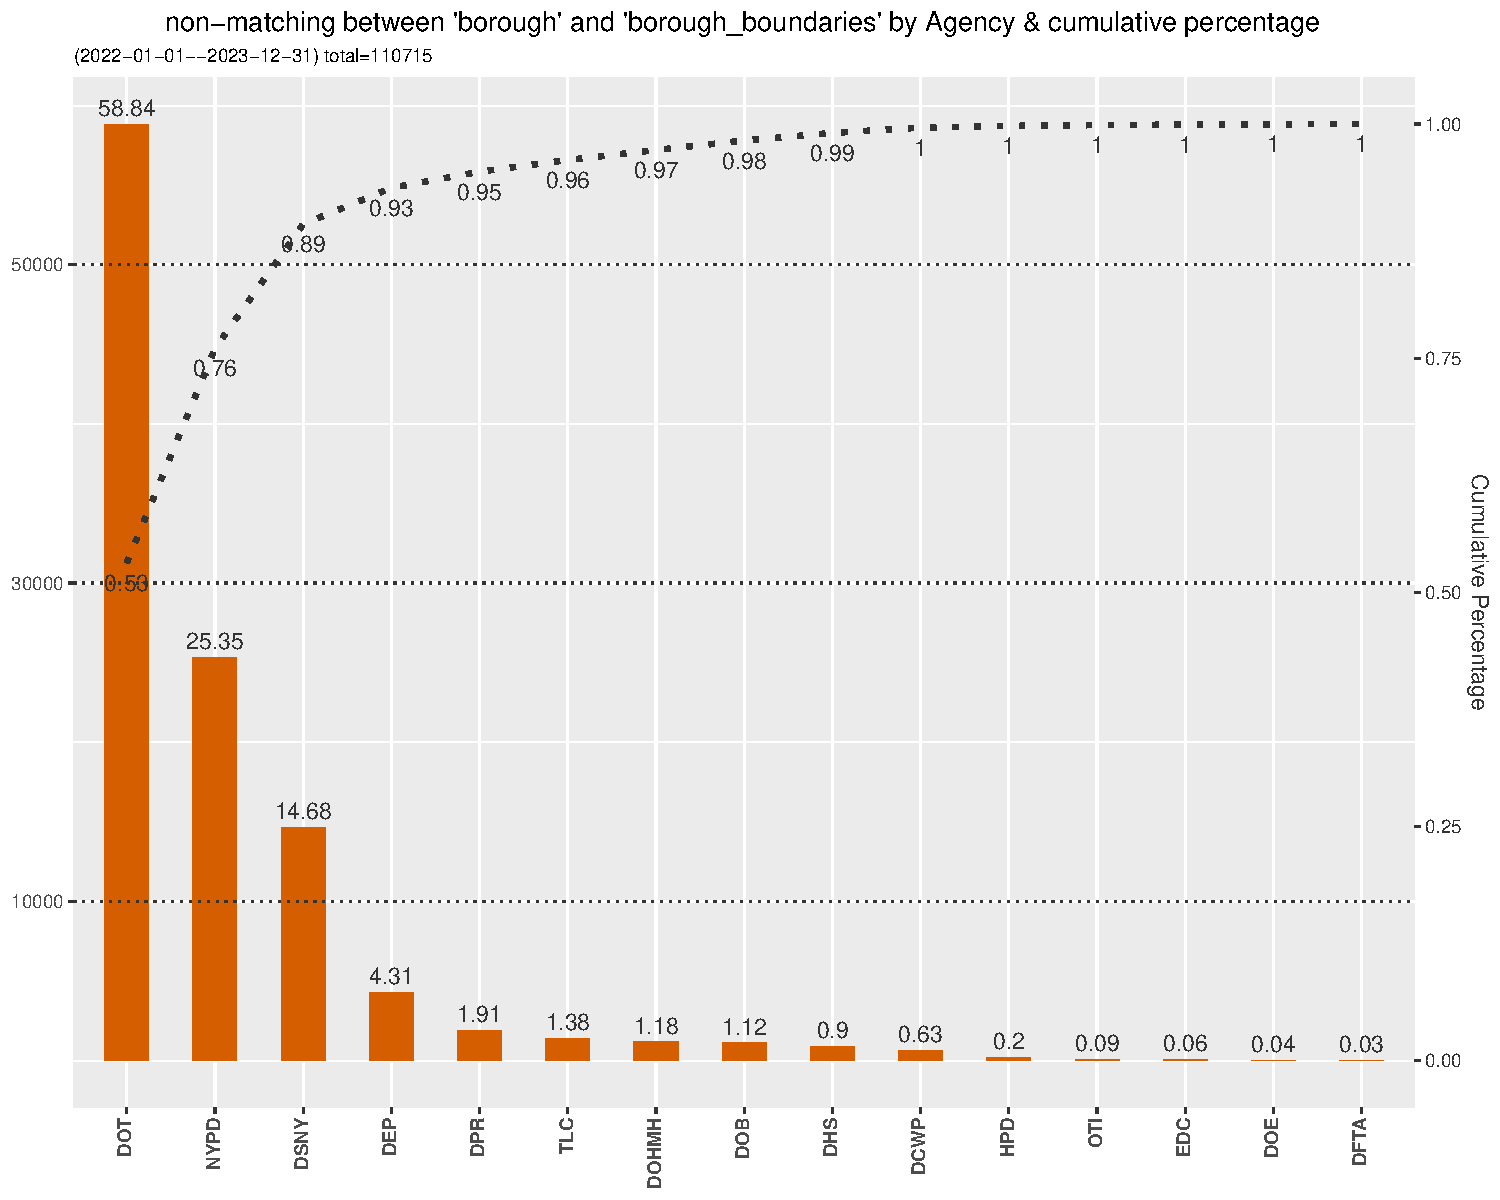
\includegraphics[width = \textwidth]{non_matching_borough_boundaries_chart.pdf}
		\caption{Non-matching borough and borough\_boundary by Agency}
		\label{fig:borough-boundaries}
	\end{figure}	
	
\subsection{borough and taxi\_company\_borough fields}
The two fields borough and taxi\_company\_borough might appear to be related. In fact, despite the names, 
the two data fields are nearly completely different with only 0.05\% matching. The mismatch is so
high that it suggests the two fields are used very differently.  This field is used exclusively by the 
Taxi \& Limo Commission which governs taxis and other cars for hire.
There are a total of 3567 non-blank entries in the taxi\_company\_borough field, with 99.94\% blank.

 \subsection{incident\_zip and zip\_codes fields}
 The zip\_code field is one of the six computed fields and its validity has been explored in Section \ref{sec:zip-codes} and
 found to be lacking with 55.55\% of the entries invalid according to the USPS, while the companion zipcode
 field incident\_zip field had an accuracy rate of 99.93\%. It is not surprising that 
 only 0.58\% of the two fields match (37,292 matches out of 6.4 million SRs.). While an Agency breakdown can be
 determined, given the questionable computation of the zip\_code field, such an analysis would
 seem to provide any useful information.  

 \subsection{police\_precinct and police\_precincts fields}  
Both the police\_precinct and police\_precincts are among the computed fields not cited in the Data Dictionary. Their usage however, is easy to discern. Are these two fields duplicates? Nearly so:  99.94\% of the entries match. Since the source of the fields and the underlying computational process are not know, it remains a challenge to determine which field is
the ``right'' field to use. (The validity of these fields is covered in Section \ref{sec:police-precincts}.)

 \subsection{agency and agency\_name fields}
 While not duplicates, these fields have a 1:1 correspondence.  The Agency field contains abbreviations for the City agencies such as NYPD, DOT, HPD, DEP, etc.
 The agency\_name field contains the full name of the various organizations: New York Police Department, Department of Transportation, Department
 of Housing Preservation and Development, Department of Environmental Protection, and so on.  Given how well known the NYC Agency abbreviations are
it seems redundant to include both in the dataset.

\subsection{landmark and street\_name}
The landmark field is listed in the Data Dictionary as ``Can refer to any noteworthy location, including but not 
limited to, parks, hospitals, airports, sports facilities, performance spaces, etc.'' We found that was not the case. To be sure
many of the entries in the landmark field do contain landmark names, e.g.``Pennsylvania Station'', ``La Guardia Airport'', 
``Gramercy Park'', the vast majority of the entries are street names, e.g. ``Fenton Avenue'', ``Steinway Street'', ``Broadway''.
These entries appear to be very similar to those in the street\_name field. And in fact, the values of street\_name
and landmark exactly match 62\% of the time, and while this is not a full duplicate, it is a precentage of 
matching that is certainly indicative of duplicate usage. Even the non-matches (excluding blanks) would appear
to be matches except for minor spelling and nomenclature changes, e.g. ``NINTH AVE'' \& ``9 AVE''.

\begin{table}[ht]
    \centering
    \caption{Non-matches between 'street\_name' and 'landmark' fields}
    \normalsize
    \begin{tabular}{>{\raggedright\arraybackslash}p{5cm} >{\raggedright\arraybackslash}p{5cm}}
        \toprule
        \textbf{street\_name} & \textbf{landmark} \\
        \midrule
        MACDOUGAL ST & MAC DOUGAL ST \\
        NINTH AVE & 9 AVE \\
        NORTH SIXTH ST & NORTH 6 ST \\
        SOUTH FOURTH ST & SOUTH 4 ST \\
        SIXTH AVE & 6 AVE \\
        THIRD AVE & 3 AVE \\
        EAST FIRST ST & EAST 1 ST \\
        FOURTH AVE & 4 AVE \\
        SAINT LAWRENCE AVE & ST LAWRENCE AVE \\
        SOUTH FIRST ST & SOUTH 1 ST \\
        BRIGHTON SEVENTH ST & BRIGHTON 7 ST \\
        WEST FIFTH ST & WEST 5 ST \\
        MT HOPE PL & MOUNT HOPE PL \\
        PENN STA & PENNSYLVANIA STA \\
        \bottomrule
    \end{tabular}
    \label{landmark}
\end{table}

The distribution by Agency for the non-matches somewhat follows the overall SR distribution (NYPD, DPR, DSNY), 
but with some notable exceptions such as Taxi \& Limo Commission, Dept of Homeless Services (DHS),
 and Dept of Health \& Mental Hygiene (DOHMH).

\begin{figure}[tbp]
		\centering
		\includegraphics[width = \textwidth]{non-matchingstreet\_nameandlandmark.pdf}
		\caption{Non-matching street\_name \& landmark by Agency}
		\label{fig:landmarkchart}
	\end{figure}	
	
	
\subsection{cross\_street\_1 \& intersection\_street\_1 and cross\_street\_2 \& intersection\_street\_2}
There are two sets of street pairs in the dataset in addition to the complaint address:

	\begin{itemize}
		\item cross\_street\_1
		\item cross\_street\_2
		\item intersection\_street\_1
		\item intersection\_street\_2
	\end{itemize}
	
These two pairs of streets are used to help identify the location of the reported incident, as it is common in
New York City to provide the street address and the cross street, as in ``24 W 90th street between Columbus and
Amsterdam''. The Data Dictionary states that these streets are
 ``based on the geo validated incident location''. It then adds ``If the service request 
pertains to a location in the middle of a block, cross street will be provided by geocoding...If the service request 
pertains to a street corner, intersection will be provided by geocoding.''  One might think that the
cross\_street(s) would apply for ``middle of a block'' incidents, while the intersection\_street(s) would
apply to those incidents that happen on a street corner; that those two sets of fields would be
exclusive to one another; and either/or situation. 

Unfortunately, that is not the case. For the majority of data rows, both pair of fields are populated and are duplicates.
In fact, 88\% of the time, cross\_street\_1 exactly matches intersection\_street\_1 and 
cross\_street\_2 exactly matches intersection\_street\_2, Only 11.9\% are non-matches.

\textit{(Note: Address standardization was applied to the street addresses using the R \emph{campfin} package. 
This was done so as to prevent the software from generating a non-match between 
streets such as ``240 E 69\textsuperscript{th} ST'' and ``240 E 69\textsuperscript{th} Street'' 
which are clearly the same address, just slight formatting and spelling differences.)}

The problem occurs when the two pairs of streets do not match, such as when one is blank and the
other is not. Which street is correct? If one is blank, say cross\_street\_1, but  intersection\_street\_1
is not blank, should you use the non-blank one?  Let's look at some examples:

\begin{table}[tbp]
    \centering
     \caption{Matching/Non-Matching cross\_street\_1 \& intersection\_street\_1}
    \normalsize
    \begin{tabular}{>{\normalsize\ttfamily}l >{\normalsize\ttfamily}l >{\normalsize\ttfamily}l}
        \toprule
        \multicolumn{3}{c}{\textbf{Matching cross\_street\_1 and intersection\_street\_1}} \\
        \midrule
        \textbf{cross\_street\_1} & \textbf{intersection\_street\_1} & \textbf{agency} \\
        \midrule
        FORT HAMILTON PKWY & FORT HAMILTON PKWY & NYPD \\
        87 ST              & 87 ST              & NYPD \\
        EAST 169 ST        & EAST 169 ST        & NYPD \\
        EAST 74 ST         & EAST 74 ST         & DOT  \\
        CHERRY AVE         & CHERRY AVE         & NYPD \\
        \midrule
        \multicolumn{3}{c}{\textbf{Non-matching cross\_street\_1 and intersection\_street\_1}} \\
        \midrule
        \textbf{cross\_street\_1} & \textbf{intersection\_street\_1} & \textbf{agency} \\
        \midrule
        KAPPOCK ST     & NETHERLAND AVE   & DOT \\
        GREENE AVE     & CLINTON AVE      & DOT \\
        LEWIS AVE      & FULTON ST        & DOT \\
        GERARD AVE     & EAST 161 ST      & DOT \\
        8 AVE          & WEST 136 ST      & DOT \\
        \bottomrule
    \end{tabular}
    \label{tab:streets1}
\end{table}

	\begin{figure}[tbp]
		\centering
		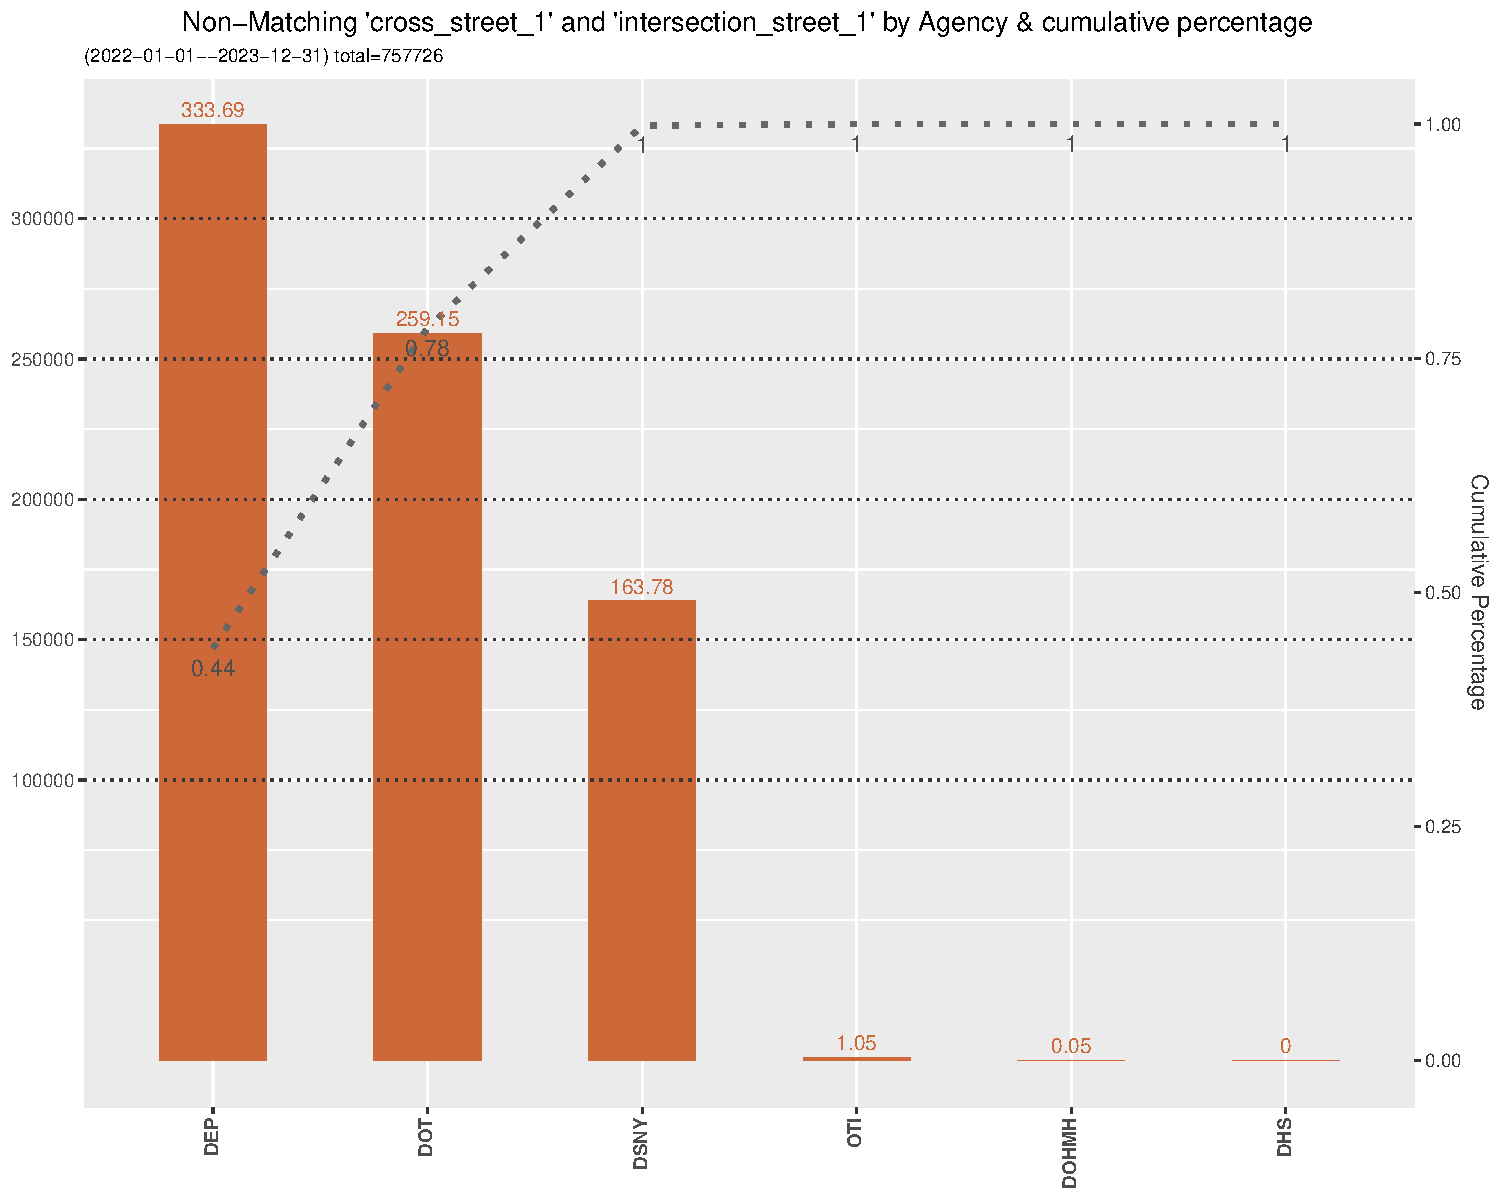
\includegraphics[width = \textwidth]{non-matchingcross_street_1andintersection_street_1.pdf}
		\caption{Non-matching X\_Street\_1 \& Intersection\_Street\_1}
		\label{fig:xstreet1}
	\end{figure}	

	\begin{figure}[tbp]
		\centering
		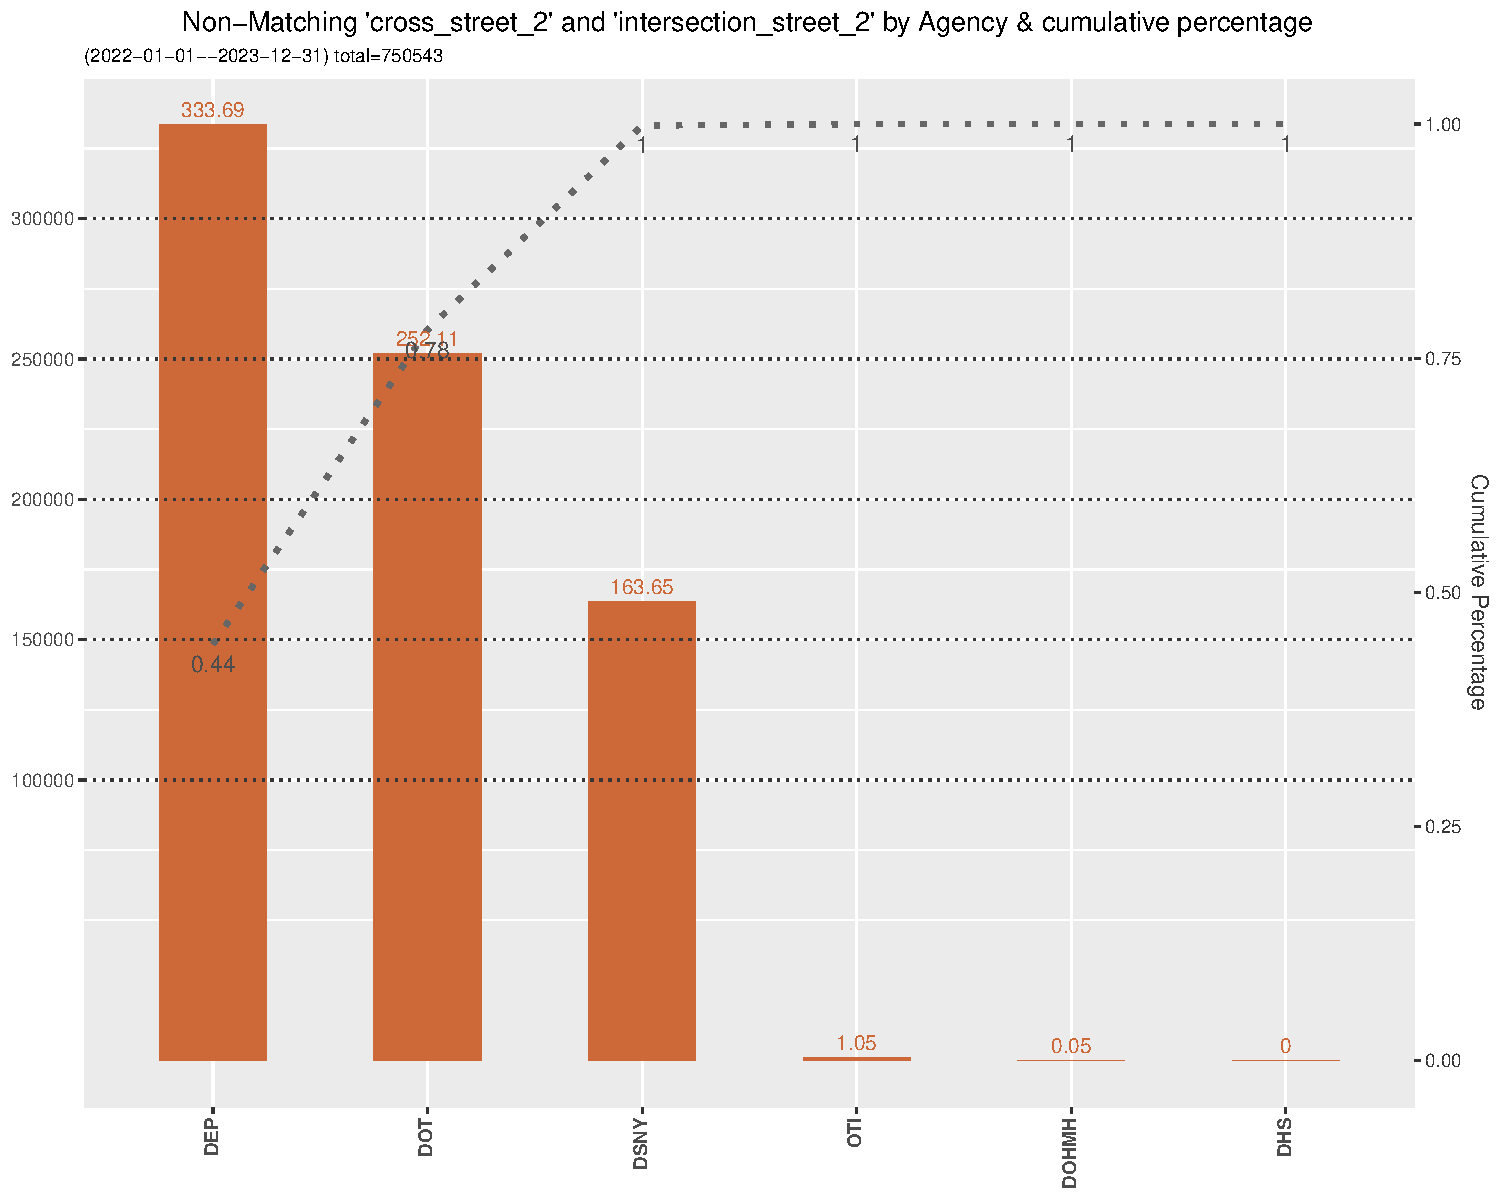
\includegraphics[width = \textwidth]{non-matchingcross_street_2andintersection_street_2.pdf}
		\caption{Non-matching X\_Street\_2 \& Intersection\_Street\_2}
		\label{fig:xstreet2}
	\end{figure}	

In addition to the matching/non-matching values, we encountered a number of what you might call
\emph{near-matches}. There were numerous cases where the cross\_street and intersection\_street
would be close to identical, e.g. HARMON DR and HARMON RD. To identify these near-matches
we applied a common method of determining matches by measuring 
the \href{https://en.wikipedia.org/wiki/Hamming_distance}{Hamming Distance} between
the two fields. The Hamming Distance is a measure of how many letters have to be changed
in order for the two fields to match. For this analysis, we chose a Hamming Distance of 2.
Here are the results for both cross\_street and intersection\_street.

\begin{table}[tbp]
    \centering
     \caption{Near-matches for cross\_street\_1, intersection\_street\_1}
    \normalsize
    \begin{tabular}{l l l r}
        \toprule
        \textbf{cross\_street\_1} & \textbf{intersection\_street\_1} & \textbf{agency} & \textbf{hamming\_distance} \\
        \midrule
        WEST 168 ST    & WEST 167 ST           & DOT    & 1 \\
        115 AVE        & 120 AVE               & DOT    & 2 \\
        105 AVE        & 107 AVE               & DOT    & 1 \\
        71 ST          & 80 ST                 & DOT    & 2 \\
        145 ST         & 150 ST                & DOT    & 2 \\
        138 ST         & 139 ST                & DOT    & 1 \\
        19 AVE         & 20 AVE                & DOT    & 2 \\
        25 AVE         & 30 AVE                & DOT    & 2 \\
        76 ST          & 79 ST                 & DOT    & 1 \\
        67 ST          & 68 ST                 & DOT    & 1 \\
        \bottomrule
    \end{tabular}
     \label{tab:x1nearmatches}
\end{table}

\begin{table}[tbp]
    \centering
    \caption{Summary of cross\_street\_1 and intersection\_street\_1}
    \normalsize
    \begin{tabular}{l r r}
        \toprule
        \textbf{category} & \textbf{count} & \textbf{percentage} \\
        \midrule
        Matching                    & 5,637,182 & 88.15     \\
        Both blank -- Matching      & 1,624,499 & 25.4      \\
        Non-matching                &   757,726 & 11.85     \\
        cross\_street\_1\_blank     &   222,232 & N/A       \\
        intersection\_street\_1\_blank &   519,348 & N/A       \\
        Near-match                  &       128 & 0.002002  \\
        \bottomrule
    \end{tabular}
    \label{tab:summary1}
\end{table}

\begin{table}[tbp]
    \centering
    \caption{Summary of cross\_street\_2 and intersection\_street\_2}
    \normalsize
    \begin{tabular}{l r r}
        \toprule
        \textbf{category} & \textbf{count} & \textbf{percentage} \\
        \midrule
        Matching -- non-blank      & 4,012,683 & 62.75     \\
        Matching -- both blank     & 1,623,276 & 25.38     \\
        Non-matching                &   750,543 & 11.74     \\
        cross\_street\_2\_blank     &   222,788 & N/A       \\
        intersection\_street\_2\_blank &   517,431 & N/A       \\
        Near-match                  &     1,500 & 0.023456  \\
        \bottomrule
    \end{tabular}
    \label{tab:summary_cross_intersection_2}
\end{table}

\begin{table}[tbp]
    \centering
     \caption{Sample of near-matching cross\_street\_2 and intersection\_street\_2 (both non-blank)}
    \normalsize
    \begin{tabular}{l l l r}
        \toprule
        \textbf{cross\_street\_2} & \textbf{intersection\_street\_2} & \textbf{agency} & \textbf{hamming\_distance} \\
        \midrule
        19 AVE         & 18 AVE                & DOT    & 1 \\
        227 ST         & 225 ST                & DOT    & 1 \\
        65 ST          & 65 PL                 & DOT    & 2 \\
        18 AVE         & 17 AVE                & DOT    & 1 \\
        BEACH 110 ST   & BEACH 109 ST          & DOT    & 2 \\
        3 AVE          & 2 AVE                 & DOT    & 1 \\
        88 ST          & 87 ST                 & DOT    & 1 \\
        WEST 114 ST    & WEST 113 ST           & DOT    & 1 \\
        192 ST         & 189 ST                & DOT    & 2 \\
        5 AVE          & 4 AVE                 & DOT    & 1 \\
        \bottomrule
    \end{tabular}
    \label{tab:near_matching_cross_intersection_2}
\end{table}


 \subsection{Shrinking file size by removing duplicates}
 
 By removing duplicate and ``near-duplicate'' fields, it is possible to shrink the file size by 12.3\%
 which for this dataset equates to a reduction of 395 Mb. A smaller file size means faster downloads,
 less storage impact, as well as simplifying data analysis efforts.  
 
 Below is a list of duplicate and near-duplicate fields. There are some challenges with these proposed deletions, 
 mostly with the ``near duplicate'' fields.  So while the park\_borough is a complete duplicate of the borough
 field, the borough\_boundary field is only 98.3\% duplicate. Admittedly, loosing 1.7\% of the data in those two
 fields is quite small, for this large dataset that amounts to 110, 715 non-matching occurrences. Similarly with 
 police\_precincts and police\_precincts where there is a 99.9\% match; close to 100\% but not a complete match.

Ultimately, it will require a deeper dive into the relationship between these duplicate and near-duplicate fields to
 determine if they can be removed or not. Pending that, the authors would propose deleting the following fields
 from the overall data set, which explanation provided.
 
 	\begin{itemize}
		    \item agency\_name: Each row of data contains the agency field, which is an abbreviation of the Agency's name.
		    The agency\_name abbreviations are clear, simple, and well understood. The authors believe the agency\_name field could
		    be eliminated without loss of data quality. 
		    
		    \item park\_borough:  This field is a 100\% match with the borough field. Removal of this field will not result in any loss
		    of data or data quality.
		    
		    \item location:  The location field is simply a concatenation of the latitude and longitude fields, with a comma and 
		    parenthesis added. The authors feel this field actually hinders data analysis as the
		    field must be re-split into the two components (latitude and longitude) to conduct geographic analysis.
		     The data is a 100\% duplication of the latitude and longitude fields. Removal of this field will
		    not result in any loss of data.
		    
		    \item police\_precinct: This field has a 99.95\% match with the police\_precincts fields. We are unable to determine which
		    field is more correct, but feel that removal of one of the precinct fields is prudent and would result in very minimal 
		    data loss. (We should note that both police\_precinct and police\_precincts fields each have 34.5\% invalid data.)
		   
		   \item borough\_boundaries (computed field): This field is one of the six computed fields. It has a 98.3 match with the
		    borough field. We recommend deleting this fields despite the somewhat limited loss of data. 
		    
		    \item cross\_street\_1 \& 2 and intersection\_street\_1 \& 2: These two pairs of fields each have an 88\% match. We would
		    recommend deleting the two intersection\_street fields while acknowledging some loss of data in doing so.
		     
		    \item zip\_codes(computed field):  This field is one of the six computed fields.  However, this field has error rate of
		    58\% and as shown in the \ref{sec:case-study-zip-codes} can lead to dangerous mistakes when used for analytical purposes.
		    We would recommend deleting this field.
	\end{itemize}
 	
Additionally, it would be worth investigating if certain data fields are in-fact useful, as the population of these fields is very, very 
scarce. For example, the taxi\_company\_borough field is 99.94\% blank, and the remaining entries match the borough field only
0.05\% field. A similar situation exists for the road\_ramp field (99.75\% blank), the vehicle\_type field (99.71\%blank), and possibly 
due\_date which is 99.62\% blank. There are several others: bridge\_highway\_direction, bridge\_highway\_name,
bridge\_highway\_segment, and taxi\_pick\_up\_location...all of which have \textgreater99\% blanks. Most of those fields appear to be 
almost exclusively used by the Taxi \& Limo Commission (TLC), which should be consulted to 
determine if those fields are used and properly populated.   



\section{Data Dictionary Observations} \label{sec:datadictionay}
During this analysis, it became apparent that the published Data Dictionary could use an update. We found many discrepancies between
the Data Dictionary and the actual data. While not actually, incorrect or dirty data, it nonetheless can lead analytic efforts astray.
In data analysis, it's essential to accurately describe the nature and purpose of each field to ensure proper handling and interpretation. 
Here are some of the noted discrepancies:  

\begin{itemize}
	\item While the Open Data portal lists the basic data types of the various fields, the Data Dictionary does not. Nor
	does it provide meaningful information on the specifics of various fields, such as constraints or domain of legal values.
	For example, the incident\_zip field is specified as ``text''. That's probably not the best definition, perhaps
	``categorical'' would be more appropriate with a description indicating that the data can contain only numeric characters
	and is not subjected to arithmetic operations. We found two instances with the zip\_code field contained character strings (``na'', ``N/A''). 

	\item Domain of legal values as contained in the Data Dictionary are incomplete. For example, the Data Dictionary indicates
	that the status field has values of assigned, canceled, closed, or pending. However, we found additional status values:
	in progress, started, and unspecified. Additionally, we discovered no SRs with a status of canceled. Similarly, the 
	address\_type field is indicated to have values address, blockface, intersection, latlong, and placename. We discovered
	additional values of bbl and unrecognized. No values of latlong were observed. Other fields suffer the same
	inaccuracies (facility\_type, vehicle\_type, taxi\_pick\_up\_location, road\_ramp, city).
\end{itemize}



\section{Recommendations} \label{sec:recommendations}
Having identified a number of data cleanliness related issues with the 311 Service Request (SR) dataset, what follows
are a series of recommendations as to how to resolve these issues. Below are those recommendations;

\begin{itemize}
	\item First, and most importantly, the Open Data Team will need to undertake a special effort to identify these data anomalies,
	confirm the veracity of the issue, and engage with the appropriate Agency Open Data Representatives to resolve these issues.
	That effort will not be easy, fast, or cheap as in some software changes will likely be required. Perhaps hardest will be
	working with the external City Agencies that feed data to the 311 SR dataset, but are not using the core 311 system.
	Integrations and API usage will need to be investigated, and in many cases the changes required to correct an issue will
	be on the source Agency side. Coordination and mutual approval of any changes will be key. Strong support from senior
	leadership will be a critical success factor.

	\item Secondly, standards will be to be identified, agreed to, and commitment to support those standards must be
	obtained. For example, what are the domain of legal values for certain fields, especially those with identified issues?

	\item Obviously, many of the data integrity issues can be resolved through rule enforcement by software. 
	For example, the software could easily prevent invalid values, such as zip codes, 
	from entering the system. Similarly for an entire range of data issues. One key area is the
	created\_date and closed\_date which are frequently cited when determining 
	responsiveness of various Agency services. The authors would argue that such dates 
	should be driven by change in ``status'', not manually entered. For example, the closed\_date is captured
	when the SR ``status'' is changed to ``closed'', and not manually entered. Such a change, along with many others, could prevent errors such
	nras negative and  zero durations which significantly affect measurements of responsiveness. 
	
	\item The large spikes in SR closure and creation occurring at midnight and noon, almost certainly point to an underlying automated
	process from an external-to-311 Agency. Such processes again distort the accurate capture of an SR duration. Data rule enforcement
	at the software integration or API level should be investigated.

	\item One possible way to have software enforce certain data standards, would be to move more non-311 Agencies to the core 311
	software system. That system was completely upgraded in 2019, and should be (relatively) easy to expand to other Agencies and usages.
	
	\item As noted, there are six ``computed'' fields in the data export that are not identified in the Data Dictionary. While these fields may be
	``experimental'', they are nonetheless present in any data portal presentation or export. As noted in this study, a number of those computed
	fields suffer from data inaccuracies. It is difficult to know what to recommend for these six field without further understanding
	of their origin, computational method, or intended usage. We would recommend updating the Data Dictionary at a minimum and
	possibly hiding those fields from public display until such time as their usage and accuracy can be ascertained.
	
	\item Removal of duplicate fields should be examined.  In some cases, such a the borough and park\_borough fields, the duplication is 100%. 
	In other cases, the duplication is in the 80-90\% range. These fields and their usage/utility should be carefully examined to determine if their
	inclusion in the 311 SR dataset is meaningful, adds value not found in other fields, and should be removed or continued to be collected.
	Initial analysis indicates that as much as 12\% size reductions are easily achievable with the removal of duplicate fields. A more thorough
	review and understanding of the fields would no doubt yield more savings. 
	
	\item Fields with extremely low data presence, such as taxi\_company\_borough which is populated only 0.06\% of the time. Similarly for several other fields 
	evaluated in this study which have a high percentage of blank/unknown values. If the presence of a small percentage of SRs 
	with these fields being populated is deemed useful and necessary, then so be it. But if the usage of these fields is so diminished, 
	then perhaps its inclusion in the 311 SR dataset is not warranted.
	
	\item The Data Dictionary is in need of an upgrade and update. The last revision is indicated at 6 March 2023, well over a year ago. 
	As noted in \textbackslash nameref: \nameref{sec:datadictionary} there are many problems with the Data Dictionary, including domain
	values, absence of the six ``computed'' fields, and inaccurate description of the usage of several fields. Some of the Data Dictionary
	entries can be undertaken immediately, which further revision should be addressed as part of a deeper data clean-up initiative. 
	
	\item The excessive precision in the latitude, longitude, and location fields is simply nonsensical.  We would recommend no more than four
	decimal places (0.000X) which represents a distance of approximately 36.4 feet. Five decimals (0.0000X) represents 3.6 feet, which 
	although possible, would be an extremely sophisticated and accurate geo-coding system. A 14 decimal number is simply a case
	of a lot of precision with limited accuracy, and should be avoided.

	\item The 10 address-related address fields (incident\_address, street\_name, city, intersection\_street\_1 \& 2, cross\_street\_1 \& 2,  landmark,
	road\_ramp, bridge\_highway\_segment, and taxi\_pick\_up\_location should be in standard USPS format. 
	There are several software packages which can standardize addresses to these standards.
	We believe such an effort should be automatically applied to these fields at data entry. This step would also greatly improve any underlying geo-coding routines which
	may be used to determine data values such as BBL, latitude, longitude, and New York State X/Y-plane coordinates.
	
	\item The use of the value ``UNKNOWN'' , ``N/A'', ``NA'', and ``na'' when entered directly as text into a field should be very carefully examined, and
	in all likelihood prohibited.  There are some indeed a few complaint\_type(s) where an ``N/A'' value is appropriate, such as a consumer\_complaint
	about certain non-geo centric issues, such as a travel agency or tax preparation service . But even in those cases a value of ``N/A'' should be 
	entered only via a drop-down menu selection. During this analysis, there were far too many data representations of missing data including: <N/A>, ``na'', `` ``,
	UNKNOWN, and ``N/A''. It's challenging for analyst to have to account for so the many different methods of representing empty or null data fields. 
	
	
\end{itemize}



\section{Protocol Suggestions} \label{sec:protocol}



\section{Discussion} \label{sec:discussion}


\bibliographystyle{asa}
\bibliography{ref}

\end{document}


